\documentclass[cn,10pt,chinesefont=nofont]{elegantbook}
\usepackage[version=4]{mhchem}
\usepackage{chemfig}
\setCJKmainfont[BoldFont={FZHei-B01},ItalicFont={FZKai-Z03S}]{FZShuSong-Z01}
\setCJKsansfont[BoldFont={FZHei-B01},ItalicFont={FZHei-B01}]{FZHei-B01}
\setCJKmonofont[BoldFont={FZHei-B01},ItalicFont={FZHei-B01}]{FZFangSong-Z02}
\setCJKfamilyfont{zhsong}{FZShuSong-Z01}
\usepackage{subcaption}
\usepackage{stmaryrd}
\title{講義}
\subtitle{仪器分析}

\author{崔洪光}
\institute{大连大学}
\date{December 31, 2020}
\version{0.3}
\bioinfo{Email}{hongguang.cui@gmail.com}

\extrainfo{A chemist thinks in open.}

\logo{du-logo.png}
\cover{cover3.jpg}

% 本文档命令
\usepackage{array}
\newcommand{\ccr}[1]{\makecell{{\color{#1}\rule{1cm}{1cm}}}}

\begin{document}

\maketitle
\frontmatter

\chapter*{特别声明}
\markboth{Introduction}{前言}

首先感谢本书\href{https://elegantlatex.org/}{Elegant\LaTeX{}} 模板,可在如下
地址获得:
\href{https://github.com/ElegantLaTeX}{GitHub}、
\href{https://ctan.org/pkg/elegantbook}{CTAN}、
\href{https://www.overleaf.com/latex/templates/elegantbook-template/zpsrbmdsxrgy}
{Overleaf} 以及 \href{https://gitee.com/ElegantLaTeX/ElegantBook}{Gitee} 上。

本讲义图片,均来自网络,在此表示对原作者的感谢!如有不妥之处,请联系我。

书籍,本没有好与坏的分别。只要用心去做,相信会有所期望。专业书籍更是如此,如
张祖德先生的《无机化学》、邢其毅先生的《基础有机化学》。“前人之述备矣”,本人也
已过了“把创作的冲动误以为创作的才能”的年龄,但,每每准备《仪器分析》课程的
时候,总是感觉那么的不顺手。市面上绝大多数的资料,总给我一种意犹未尽,或是
如鲠在喉的感觉。尤其其中数据处理的部分,其表现坐实了“化学就是动手实验的学科”,
或是“没什么理论基础”。对应于时下流传的“环化生材四大天坑专业”,尴尬之处在于,
这四个专业所必须的分析验证手段(即仪器分析),都不是本专业开发出来的。念及,
这种冲动又开始砰砰然。那就从一份认真的讲义开始吧!


\vskip 1.5cm

\begin{flushright}
Hongguang Cui\\
December 20, 2020
\end{flushright}

\setcounter{tocdepth}{3}
\tableofcontents
%\listofchanges

\mainmatter
\chapter{光分析导论}
\begin{introduction}[重点]
    \item Beer-Lambert定律
    \item 数据处理方法
    \item 光学系统
\end{introduction}
\begin{introduction}[难点]
    \item 标准曲线法
    \item 标准加入法
    \item 内标法

\end{introduction}
\section{电磁辐射与物质的相互作用}
从对彩虹的观察中我们知道,可见光(白光)由从紫色到红色的连续颜色组成。如果一束
白光通过水烧杯,保持白色。如果将高锰酸钾添加到水中,白光穿过溶液后会变成紫色。
高锰酸盐溶液允许白光的红色和蓝色成分通过,但会吸收原始光束中的其他颜色。
这是\emph{电磁辐射}或光与物质相互作用的一个例子。在这种情况下,电磁辐射是可见光
,我们可以用眼睛看到吸收某些光的效果。但是,电磁辐射与物质之间的相互作用以多种
方式发生,并且辐射能范围很广。这些相互作用中的大多数不是人眼可见的,而是可以
用合适的仪器测量的。

电磁辐射与物质的相互作用不是偶然的,而是关于吸收或发射的光的波长,以及吸收或
吸收的程度遵循有据可查的规则。光谱学的主题是电磁辐射与物质相互作用的研究。

\subsection{电磁辐射}
多年以来,电磁辐射的性质使科学家感到困惑。有时,光看起来像波;在其他时候,它的
行为好像是由小颗粒组成的。尽管我们现在已经了解包括电磁辐射在内的所有物质的
“波粒二象性”,但从量子力学的角度来看,在许多情况下将电磁辐射视为具有波的属性
仍然很方便。可以表示光波为振荡垂直的电场和磁场。场彼此成直角,并且与光的传播
方向成直角。
\begin{figure}[htbp]
    \centering
    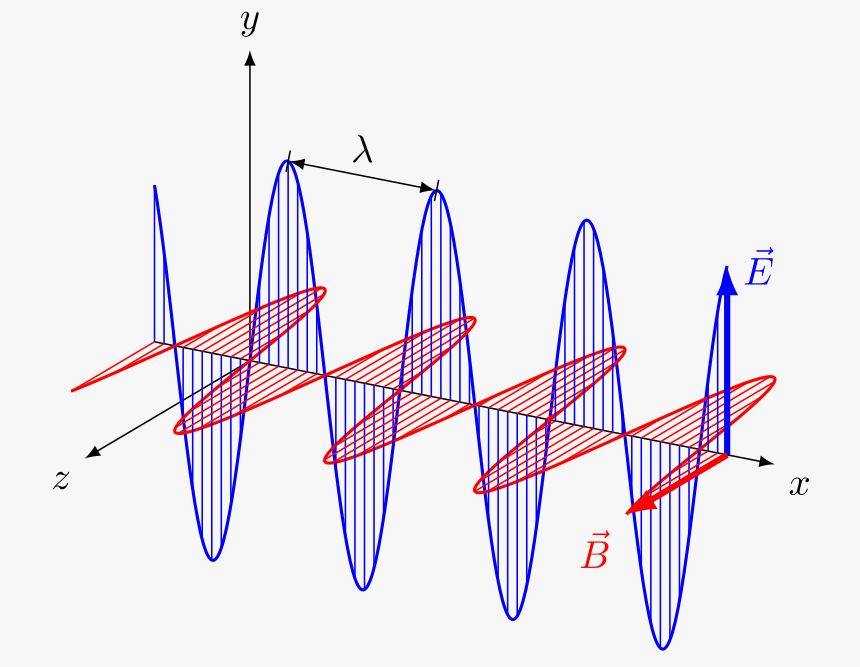
\includegraphics[width=0.85\textwidth]{ElectromagneticWavesPropagation.png}
    \caption{光沿着$x$方向传播,$y$方向为电场,$z$方向为磁场,$\lambda$为波长}
    \label{fig:EMwave}
\end{figure}

如图\ref{fig:EMwave}所示,振荡为正弦曲线。我们可以轻松、准确地测量波长$\lambda$
,定义为两个
连续最大值之间的波峰到波峰的距离。波长的标准单位是长度的SI单位,米($m$),
但是通常使用较小的单位,例如厘米($cm$),微米($\mu m$)和纳米($nm$)。波的
振幅定义为从原点到振荡的点位移的矢量的最大值。仅沿一个轴传播的光波
电场部分的示例如图\ref{fig:EMwave}所示。仅限于一个平面的这种波称为平面偏振光。
所示的波仅代表单个波长$\lambda$。仅一种波长的光称为单色光。包含多个波长的光
称为多色光。白光是多色光的一个示例。波的频率$\nu$是每秒通过固定点的波峰数。
波的波峰间振荡称为周期。频率的通用单位是赫兹($Hz$)或倒数秒($s^{-1}$);
频率的较旧术语是每秒的周期数($cps$)。一赫兹等于每秒一个周期。
光的波长$\lambda$和频率$\nu$满足下式
\begin{equation}
    c = \lambda\nu
    \label{eq:1st}
\end{equation}
其中,$c$为真空中光速,$2.997\times 10^8 m/s$;$\nu$频率,单位为$Hz$;$\lambda$
波长,单位为$m$。

真空中,光速最大,且与波长无关。频率由光源决定,并且不会变化。当光通过非真空的
材质,其速度会降低。因为频率不能改变,波长减小。空气中的光速,它与
真空中的光速相差很小。通常,我们将$3.00\times 10^8 m/s$(三位有效数字)用于空气
或真空中的光速。在某些情况下,将光视为粒子流会更方便。光的粒子成为光子。光子的
特征在于能量$E$与频率有关,关系式如下:
\begin{equation}
    E = h\nu
    \label{eq:2nd}
\end{equation}
其中,$E$为能量,单位是$J$,$h$是普朗克常数,$6.626\times 10^{-34} Js$,$\nu$
是频率,单位是$Hz$。联立式(\ref{eq:1st})和(\ref{eq:2nd}),可得
\begin{equation}
    E = \frac{hc}{\lambda}
    \label{eq:3th}
\end{equation}
\begin{figure}[htbp]
    \centering
    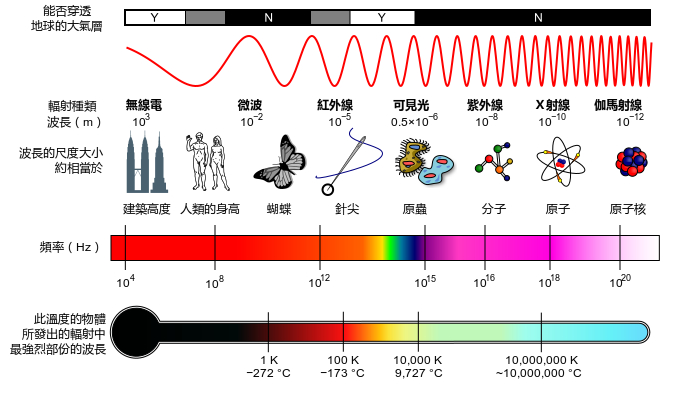
\includegraphics[width=0.85\textwidth]{wave.jpg}
    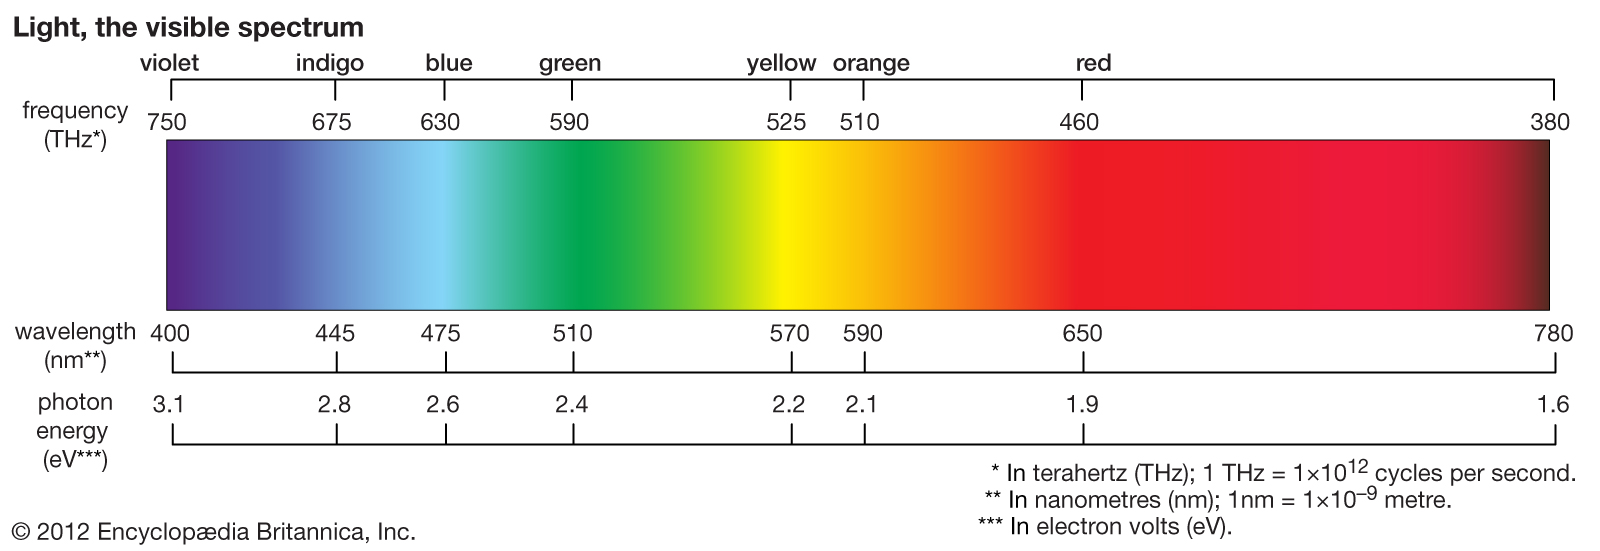
\includegraphics[width=0.85\textwidth]{visual.jpg}
    \caption{电磁波谱}
    \label{fig:wavegraph}
\end{figure}
从式(\ref{eq:2nd})和(\ref{eq:3th})的关系可以看出,电磁辐射的能量与频率成正比,
与波长成反比。电磁辐射的范围从极低能量(长波,低频)的辐射(如无线电波和微波)
到极高能量(短波,高频)的辐射(如X射线)。作为分析化学家,我们感兴趣的电磁谱
的主要区域如图(\ref{fig:wavegraph})所示。从该图清楚可见,可见光,即人眼所响应
的电磁频谱的一部分,仅占所有辐射能的很小一部分。表(\ref{tab:1st})列出了各种类
型电磁辐射的一些常用单位和符号。
\begin{table}[htbp]
    \centering
    \caption{电磁辐射波长符号和单位}
    \label{tab:1st}
    \begin{tabular}{lccl}
        \hline
        {\bf Unit}&{\bf Symbol}&{\bf Length ($m$)}&{\bf Type of Radiation}\\
        \hline
        Angstrom & \AA& $10^{-10}$&x-ray\\
        Nanometer& $nm$& $10^{-9}$&UV/Vis\\
        Micrometer& $\mu m$& $10^{-6}$&Infrared (IR)\\
        Millimeter& $mm$& $10^{-3}$&IR\\
        Centimeter& $cm$& $10^{-2}$&Microwave\\
        Meter& $m$& $1$&Radio\\
        \hline
    \end{tabular}
\end{table}
\subsection{电磁辐射与物质的相互作用}
光谱学是研究辐射能(光)与物质相互作用的方法。从量子力学中我们知道,能量实际上
只是物质的一种形式,所有物质都具有波和粒子的特性。但是,由以固体,液体或气体
形式存在的分子,原子或离子组成的物质主要表现出粒子的特性。光谱学研究光与物质的
相互作用,物质定义为由分子或原子或离子组成的材料。

在气体中,原子或分子彼此广泛分离;在液体和固体中,原子或分子紧密相连。在固体中
,原子或分子可以像许多矿物中那样排列成高度有序的阵列(称为晶体),也可以像许多
塑料中一样无规排列或无定形。无论原子,分子和离子的物理状态或排列如何,它们都在
不断运动。对于分子,涉及许多类型的运动。分子可以转动,振动和平移(在空间中到处
移动)。与辐射能的相互作用会影响这些分子运动。吸收红外辐射的分子振动幅度更大;
与UV/VIS光的相互作用可将键合电子移动到分子中更高的能级。任何形式的运动或电子能
级的变化都涉及分子能量的变化。能量的这种变化称为\emph{跃迁}。分子有可能发生
振动跃迁,转动跃迁和电子跃迁。原子和离子也有一些相同类型的运动。原子可以在
空间中移动,其电子可以在能级之间移动,但是原子和单原子离子不能转动或振动。
物质的化学性质(其组成),其物理状态以及处于物理状态的原子或分子彼此之间的
排列会影响任何给定材料与电磁辐射相互作用的方式。表\ref{tab:2nd}列出了通过光谱
学研究的一些重要的跃迁类型。我们将在后面的章节中详细介绍这些技术。实际上,有数
百种用于研究物质的跃迁类型和光谱学类型,我们介绍最常见的分析光谱类型。

\begin{table}[htbp]
    \centering
    \caption{光谱研究的几种典型转换}
    \label{tab:2nd}
    \begin{tabular}{lll}
        \hline
        转换类型& 光谱方法 & 波长范围 \\
        \hline
        磁场中核子自旋 & 核磁共振 & $0.5-10 m$\\
        分子转动与振动 & 拉曼和红外 & $0.8-300 \mu m$\\
        成键电子和价电子能级 & UV/VIS & $180-800 nm$\\
        核心电子能级 & X-ray & $0.1-100 $\AA\\
        \hline
    \end{tabular}
\end{table}

当光照射到物质样品上时,光可能会被样品吸收,透射穿过样品,从样品表面反射或
被样品散射。样品在吸收入射光后也可以发光。这样的过程称为\emph{发光}。根据发生
的特定过程,有不同类型的发光,称为\emph{荧光}或\emph{磷光}。发光也可能是由吸收
光以外的过程引起的。有基于所有这些相互作用的光谱方法。表\ref{tab:3th}总结了
光与物质相互作用的主要类型,并给出了基于这些相互作用的常见光谱技术的示例。
目前,我们将专注于物质对光的吸收、透射和发射。

\begin{table}[htbp]
    \centering
    \caption{几种光与物质的作用}
    \label{tab:3th}
    \begin{tabular}{lll}
        \hline
        相互作用 & 测量的辐射 & 光谱方法 \\
        \hline
        吸收(Absorption) &
        入射光(Incident light) $I_0$ & 原子吸收(Atomic absorption)\\
        传输(Transmission)&透射光(Transmitted light) $I$&分子吸收(Molecular absorption)\\
        \hline
        \multirow{3}*{\shortstack{吸收后发射\\(Absorption\\ then emission)}} & 
        \multirow{3}*{发射光(Emitted light) $I'$} & 原子荧光(Atomic fluorescence)\\
        &&分子荧光(Molecular fluorescence)\\
        &&分子磷光(Molecular phosphorescence)\\
        \hline
        \multirow{3}*{散射(Scattering)} &
        \multirow{3}*{散射光(Scattered light) $I_S$} &测浑法(Turbidimetry) \\ 
        &&浊度法(Nephelometry)\\
        &&拉曼(Raman)\\
        \hline
        \multirow{2}*{反射(Reflection)}&\multirow{2}*{反射光$I_R$}&全反射衰减
        (Attenuated total reflection)\\
        &&漫反射(Diffuse reflection)\\
        \hline
        \multirow{3}*{发射(Emission)}&\multirow{3}*{发射光(Emitted light)$I_e$}
        &原子发射(Atomic emission)\\
        &&分子发射(Molecular emission)\\
        &&化学发光(Chemiluminescence)\\
        \hline
    \end{tabular}
\end{table}

如果我们将白光(即可见光)穿过蓝色玻璃,则发出的光就是蓝色。玻璃吸收了其他颜色
,例如红色和黄色。我们可以通过蓝色玻璃发出红色光来确认这种吸收。如果吸收足够强
,则所有的红光都会被吸收;玻璃上没有光发出,而是黑色。如何解释呢?

电磁辐射与物质的相互作用符合量子力学定律。原子、离子和分子,以具有特定能量的某
些离散状态存在。依据量子力学定律,状态的改变需要吸收或发射能量$\Delta E$,该能
量等于始态和终态之间的能量差。能量状态是量子化的,状态变化(能量变化)可表示:
\begin{equation}
    \Delta E = E_{\text{final}} - E_{\text{initial}} = h\nu
    \label{diffEnergy}
\end{equation}
将$c = \lambda\nu$带入式(\ref{diffEnergy}),得
\begin{equation}
    \Delta E = h\nu=\frac{hc}{\lambda}
    \label{diffEnergy2}
\end{equation}
从式(\ref{diffEnergy2})可知,物质在两种状态跃迁时,吸收或发射辐射。物质仅仅能
吸收或发射特定频率(或波长)的辐射,对应于物质存在的两种状态的能量差。吸收辐射
$E_{\text{final}} > E_{\text{initial}}$,发射辐射$E_{\text{final}} <
E_{\text{initial}}$。$\Delta E$有正有负,在求解转换的波长和频率时,使用绝对值。
波长、频率和光速,总是正值。

特定的分子,如正己烷,或是特定的原子,如汞,能吸收或发射特定频率的辐射。所有正
己烷吸收和发射的频率是相同,这些频率不同于其它分子,例如苯。所有汞原子吸收相同
频率的入射光,这一频率与其它原子(如铅、铜)不同。不但频率是独特的,吸收或发射
的度也是独特的。给定强度的光的吸收或发射的度。化合物频率的独特性和每一个频率下
的吸收和发射的总量,是表征化合物的光谱学基础。我们称频率和强度为吸收或发射
光谱。

分子或原子最低能量状态称为基态。比基态高的,称为激发态。通常,室温下,分子和原子
都处于基态。

前例中蓝色玻璃能吸收红光和黄光,我们粗略的推测能量状态图。假设任何一种或几种光
穿过玻璃前,玻璃是基态,能量为$E_1$。玻璃吸收红光后,到达激发态,激发态与基态的
能量差为红光波长所具有的能量。从图\ref{fig:wavegraph}中,在可见光区域,选择一个
红光的波长,如$653 nm$。玻璃吸收$\lambda = 653 nm$的光,计算频率为
\[
    \nu =\frac{c}{\lambda} = \frac{2.997\times 10^8 m/s}{(653 nm)\times
    (10^{-9} m/nm)}=4.59\times10^{14}s^{-1}
\]
通过频率,我们可以计算激发态$E_2$和基态的能量差
\[
    \begin{array}{l}
        \Delta E = E_2 - E_1 = h\nu\\
        \Delta E = (6.626 \times 10^{-34}J s)(4.59\times 10^{14}s^{-1})\\
        \Delta E = 3.05 \times 10^{-19} J
    \end{array}
\]
同理,我们假定玻璃吸收$575 nm$的黄光(对应$5.21\times 10^{14} Hz$频率),到激
发态能量为$E_3$,与基态能量差为
\[
    \begin{array}{l}
        \Delta E = E_3 - E_1 = h\nu\\
        \Delta E = (6.626 \times 10^{-34}J s)(5.21\times 10^{14}s^{-1})\\
        \Delta E = 3.45 \times 10^{-19} J
    \end{array}
\]
根据以上两组数据,可以构建一个简单的蓝玻璃能级图,如图\ref{fig:EnergyDia}。

\begin{figure}[htpb]
    \centering
    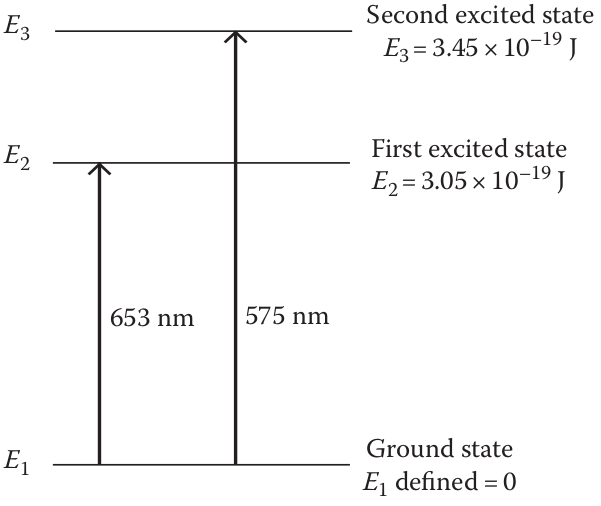
\includegraphics[width=0.5\textwidth]{2020-12-25_18-46.png}
    \caption{简单能级图}
    \label{fig:EnergyDia}
\end{figure}

图中显示两个激发态:一个对应蓝色玻璃吸收$653 nm$波长的光,另一个对应吸收$575 
nm$。玻璃不吸收蓝光,图中没有任何涉及到蓝光的能量状态。红光的吸收发生在$620$到
$750 nm$,黄光的吸收发生在$550$到 $590 nm$,如此类推。实验中,为什么分子吸收
光谱是宽频的呢?玻璃吸收可见光,归因于分子中价电子的激发,或者说电子跃迁。电子
跃迁比转动和振动需要更多的能量,转动$<$振动$<$电子。图\ref{fig:EnergyDia2}更
接近实际的能级图。
\begin{figure}[htpb]
    \centering
    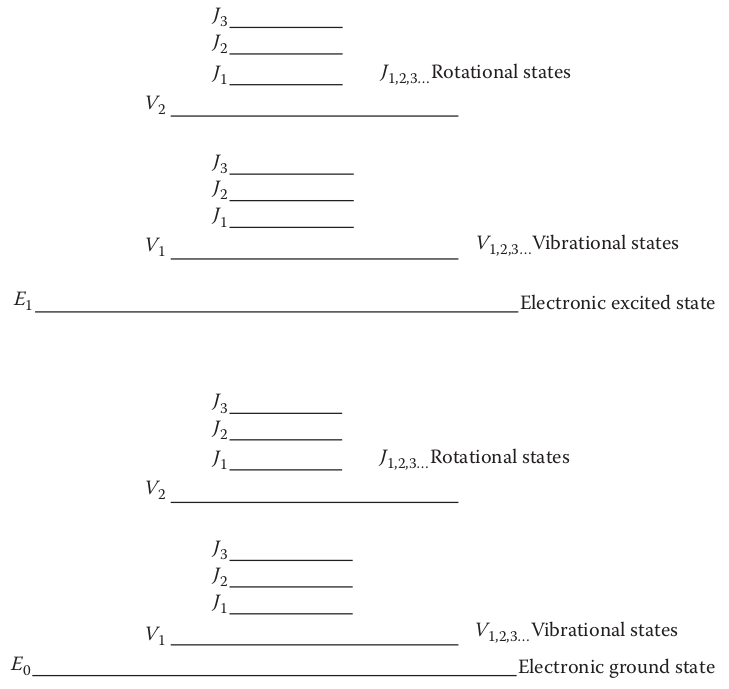
\includegraphics[width=0.55\textwidth]{2020-12-25_21-55.png}
    \caption{分子能级图,$E_{0,1,2,\dots}$表示各电子能级,$V_{1,2,3,\dots}$振动
    子能级,$J_{1,2,3,\dots}$为转动子能级}
    \label{fig:EnergyDia2}
\end{figure}
对于每一个电子态$E_n$都有许多转动和振动子能级。每一个子能级之间由很小的能量差异
,从一个能级$E_n$跃迁至另一个较高的能级,不是单一的能量,电子可以停留在
任意子能级上,从而导致是一个能量范围。所以,分子对红光的吸收,在一定的波长范围
内,而不是单一的、离散的波长。

激发态能量不稳定,分子或原子需要回到最低能量状态,并释放出能量,通常是以发光的
形式。激发态很短暂,在$10^{-9}$到$10^{-6} s$的范围内。

分子或原子吸收符合$\Delta E = h\nu = hc/\lambda$的辐射能时,便可绘制吸收光谱。
物质的吸收光谱展示了吸收的光的能量(频率或波长),以及在每个频率或波长下吸收
多少光。分子或原子的性质,决定在给定条能量下吸收光的量。物质的完整光谱包括
吸收的能量和吸收光的相应强度。纵轴表示强度变化,横轴表示频率或波长的变化。强度
与能量的关系图,就是我们通常说的光谱。聚苯乙烯的红外吸收光谱和苯的紫外吸收光谱
显示在图\ref{fig:example1}。
\begin{figure}[htpb]
    \centering
    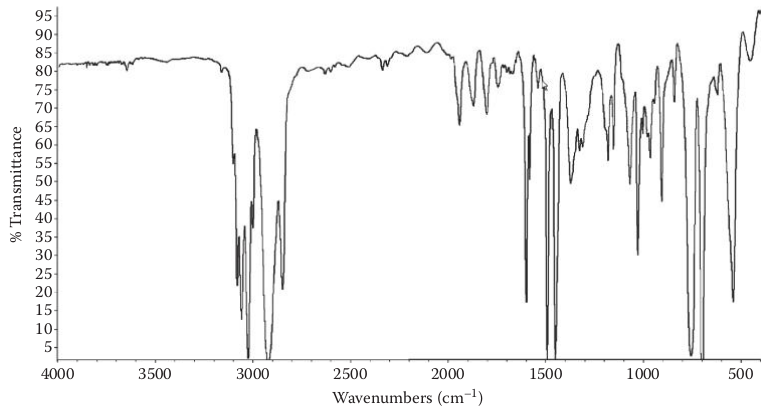
\includegraphics[width=0.85\textwidth]{2020-12-25_23-36.png}\\
    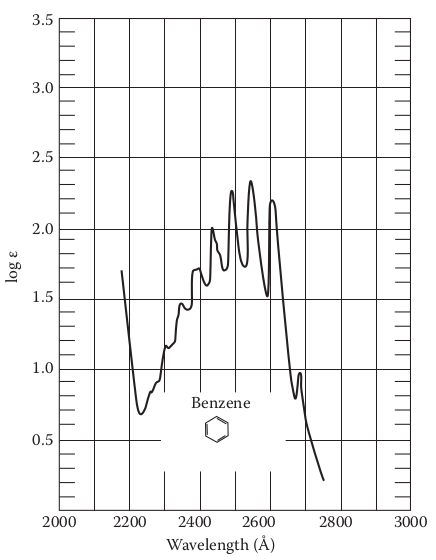
\includegraphics[width=0.65\textwidth]{2020-12-25_23-38.png}
    \caption{吸收光谱示例}
    \label{fig:example1}
\end{figure}

当处于激发态的原子或分子通过发射辐射能返回基态时,可获得发射光谱。发射光谱可
由形成激发态的许多不同方式产生。原子和分子不仅可以通过吸收电磁辐射来激发,而且
还可以通过原子和分子之间的碰撞而引起的能量转移,通过添加热能以及通过添加来自
放电的能量来激发。几种类型的发射光谱中使用了不同的激发方法,将在后面的章节中
详细讨论。在吸收电磁辐射激发后,原子或分子发射电磁辐射是一个特殊的术语。
这种发射称为发光。换句话说,如果将光用作激发的源,则将光的发射称为发光
(luminescence);如果使用其他激发源,则光的发射称为简单发射(emission)。

\section{原子和原子光谱}
核与绕核运动的电子构成原子。每一种元素都有特定的核电荷数,即电子数和质子数。
电子在不同的原子轨道运动,具有不同的能量,电子的能量态是量子化的。最低能量,
元素最稳定的电子构型称为基态。在无机化学中,我们已经学习基态原子电子构型,
遵循能量最低原理、保里不相容原理和洪特规则。例如,基态钠原子电子构型为
$1s^22s^22p^63s^1$;基态钾原子电子构型为$1s^22s^22p^63s^23p^64s^1$;
基态钒原子电子构型为$1s^22s^22p^63s^23p^64s^23d^3$,诸如此类。原子吸收光的能量
,外层(价)电子从基态跃迁至较高能量轨道,即能量高、不稳定的激发态。电子要从
激发态返回基态,电子放出能量。这个能量,在量上等于激发态和基态两个能级的差值。
该过程如图\ref{fig:2.5}所示。如果释放能量是以电磁辐射的形式,电子跃迁就满足
式(\ref{diffEnergy})和(\ref{diffEnergy2})
\begin{equation}
    \Delta E = E_{\text{final}} - E_{\text{initial}} = h\nu =
    \frac{hc}{\lambda}
    \label{eq:2.6}
\end{equation}
每种元素因其独特的电子构型,都有独特的所允许的电子能级。吸收或发射的光的波长,
是该元素特征属性。原子对辐射能的吸收,称为原子吸收光谱,将在后续章节学习。
\begin{figure}[htpb]
    \centering
    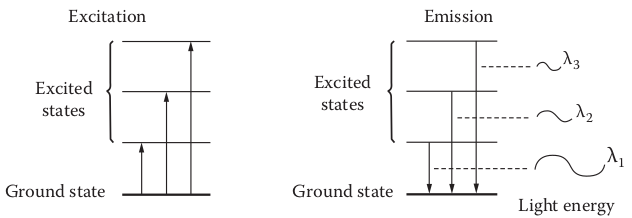
\includegraphics[width=0.8\textwidth]{2020-12-26_17-26.png}
    \caption{原子内能量跃迁}
    \label{fig:2.5}
\end{figure}

实际上,原子精确的能级图,是激发态原子的发射光谱。图\ref{fig:2.6}显示汞原子的
能级图。需要注意的是,原子没有转动和振动子能级。电子被激发到较高的激发态,
能量的变化非常明确,吸收(或发射时弛豫到基态)的波长可以认为是单色光。原子的
价电子跃迁所涉及的波长落在光谱的可见区和紫外区,该区域通常简称为UV/VIS。确定
所有元素的能级图,并提供原子吸收和发射的波长表,附录列出用于原子吸收光谱测量
的吸收波长。
\begin{figure}[htpb]
    \centering
    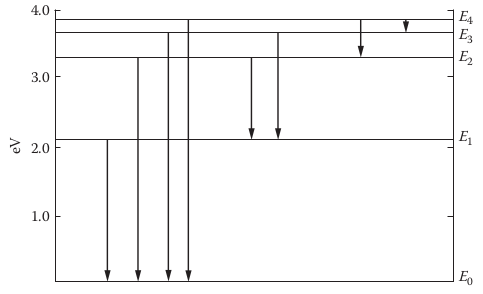
\includegraphics[width=0.65\textwidth]{2020-12-26_18-22.png}
    \caption{汞原子能级图}
    \label{fig:2.6}
\end{figure}

已知样品吸收或发射光的波长,可以对样品中存在元素进行定性鉴定。测量在给定波长
处吸收或发射的光的强度,可以给我们元素定量的信息。原子光谱法(吸收、发射和
荧光)灵敏度非常高,检测极限为$10^{-12}$到$10^{-15}$克。

原子有可能在X射线区域吸收更高能量的辐射。这样的吸收可能导致内壳(核)电子被
激发,随后发射X射线。此过程构成X射线荧光(XRF)光谱。
\section{分子和分子光谱}
与分子相关的能量状态,像原子一样,也被量子化。使用无线电波到紫外区域的辐射
来研究分子中允许状态之间跃迁的光谱方法非常强大。这些方法提供有关分子定性和
定量的信息,包括有关分子结构的详细信息。
\subsection{转动跃迁}
分子在空间中转动具有相关的转动能。分子可能仅以离散(量子化)的转动能态存在。
吸收适当的能量会导致从较低能量的转动状态过渡到较高能量的转动状态,其中分子
转动得更快。该过程引起转动吸收光谱。分子的转动能量取决于其角速度,该角速度
是可变的。转动能量还取决于分子的形状和重量分布,它们随键角的变化而变化。
尽管在\ce{O2}等双原子分子中形状的变化受到限制,但具有两个以上原子的分子
(例如己烷,\ce{C6H14})具有许多可能的形状,因此具有许多可能的转动能级。
此外,分子中原子中不止一个自然同位素的存在会产生新的一组转动能级。
碳就是这种情况,其中含碳分子中,小百分比原子的碳原子是\ce{^{13}C}而不是
\ce{^{12}C}
。因此,即使是简单的分子也具有复杂的转动吸收光谱。转动变化涉及的能量非常小,
每个分子约$10^{-24}J$。因此,吸收的辐射位于频谱的射频(RF)和微波区域。
由于所涉及的实验困难和所产生光谱的复杂性,在分析化学中尚未充分利用微波光谱法。
该技术仅限于气相,并且被射电天文学家用来检测星际云中的化学物质。
\subsection{振动跃迁}
\begin{figure}[htpb]
    \centering
    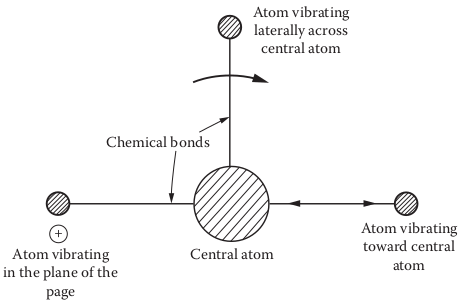
\includegraphics[width=0.7\textwidth]{2020-12-26_19-17.png}
    \caption{分子中成键原子可能的振动}
    \label{fig:2.7}
\end{figure}
可以将分子视为通过弹簧(化学键)连接在一起的一组重物(原子)。原子可以朝着
压缩和拉伸两个方向彼此振动,或者以各种角度彼此弯曲,如图\ref{fig:2.7}所示。
每个这种振动都具有与之相关的特征能量。量子化与分子振动相关的振动能态。分子的
振动能的变化与光谱的红外区域辐射能的吸收有关。虽然红外辐射的吸收会引起吸收
分子的振动发生变化,但振动能的增加通常还伴随着分子转动的增加。转动能级是振动
能级的子能级,如图\ref{fig:EnergyDia2}所示。因此,实际上,红外辐射的吸收对应
于分子中转动能和振动能变化的组合。由于具有两个以上原子的分子具有许多可能的
振动状态,因此红外吸收光谱很复杂,由多个吸收带组成。分子吸收红外辐射是光谱学
中最重要的技术之一。通过红外吸收光谱,可以推断出分子的结构,并且可以进行分子
的定性鉴定和样品分子组成的定量分析。
\subsection{电子跃迁}
当原子结合形成分子时,各个原子轨道结合形成一组新的分子轨道。在结合核的平面内,
沿着连接结合核的轴具有电子密度的分子轨道称为sigma($\sigma$)轨道。具有在键合核
平面之上和之下的电子密度的那些分子轨道称为pi($\pi$)轨道。$\sigma$和$\pi$轨道可
能有两种类型:成键轨道或反键轨道。成键轨道的能量低于相应的反键轨道。当将分子中
的电子分配给轨道时,最低能量的成键轨道首先被填充。有关分子轨道理论的综述,请
参阅无机化学。

在温度和压力的正常条件下,分子中的电子处于基态构型,填充了可用
的最低能量的分子轨道。吸收适当的辐射能会导致外部电子被提升为更高能量的激发态。
与原子一样,引起分子电子跃迁所需的辐射能位于可见光和紫外线区域。与原子一样,
分子的激发态没有基态稳定。分子将自发还原(弛豫)到发射UV/VIS辐射能的基态。
与原子不同,分子中的能量状态具有转动和振动子能级,因此当分子的电子被激发时,
振动和转动能通常会同时发生变化。总的能量变化是电子的、转动的和振动的能量转变。
分子具有许多可能的转动和振动状态,大量分子对UV/VIS辐射的吸收(每个分子的转动和
振动状态略有不同)会导致在很宽的波长范围内吸收,这称为吸收带。分子的UV/VIS吸收
光谱通常具有几个宽吸收带,与红外光谱相比非常简单。分子吸收和发射光谱可以用
于化学物种的定性鉴定。这项技术曾经是用于确定有机分子结构的主要方法之一,但
已被功能更强大且普遍使用的NMR、IR和MS替代。UV/VIS吸收光谱常用于样品分子组成的
定量分析。分子荧光光谱是一种灵敏度极高的方法,具有检测单个分子的能力。
\section{吸收定律}
光束的辐射功率$P$定义为单位面积内每秒的光束能量。相关的量是强度$I$,即每单位
立体角的功率。功率与强度都与光波振幅的平方有关,并且吸收定律可以用功率或
强度来表示。我们使用强度$I$,其它文献中,可能会看到用$P$的幂的形式。

\begin{figure}[htpb]
    \centering
    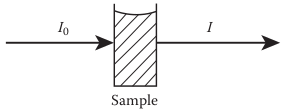
\includegraphics[width=0.4\textwidth]{2020-12-27_09-16.png}
    \caption{吸收示例}
    \label{fig:2.8}
\end{figure}

光通过吸收样品时,透射光的强度会降低。假设单色器光束(单一波长)强度为$I_0$,
样品吸收这一波长的辐射,如图\ref{fig:2.8}。透射光强度为$I$,$I_0 \geq I$。
如果样品不吸收辐射,$I = I_0$。吸光度$T$为
\begin{equation}
    T = \frac{I}{I_0}
    \label{2.7}
\end{equation}
透射率是入射光通过样品后的一个分数,取值范围为0到1。即使$I_0$发生变化,
$I/I_0$这一比例也会保持相对恒定。也就是说,$T$是不依赖实际强度$I_0$。研究
物质吸收的量,另一个物理量是吸光度$A$
\begin{equation}
    A=\log{\left(\frac{I_0}{I}\right)}
    =\log{\left(\frac{1}{T}\right)}=-\log{T}
    \label{2.8}
\end{equation}
没有光吸收,$I=I_0$,$A=0$。百分比透射率,$\% T$,等于$T\times 100$,百分比
吸光度,$\% A$,等于$100-\%T$,也常用于光谱中。
\begin{problem}
    假设有一水溶液吸收样品放置于底面边长为1 cm正方形的玻璃样品池中,如图
    \ref{fig:2.9}。光程$b$,入射光$I_0$强度为100,经过第一个样品池,有50\%的光被
    吸收,有50\%光透过。透射光$I_1$为50强度单位,所以,$\% T = 50$
    \begin{figure}[htpb]
        \centering
        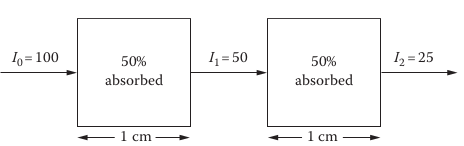
\includegraphics[width=0.75\textwidth]{2020-12-27_09-43.png}
        \caption{双样品吸收}
        \label{fig:2.9}
    \end{figure}
    \[
        \begin{array}{l}
            T = \frac{\% T}{100} = \frac{I_1}{I_0}\\
            T = \frac{50}{100} = 0.50
        \end{array}
    \]
    通过$T$计算吸光度
    \[
        A = -\log{T} = -\log{\left(0.50\right)} = 0.30
    \]
    第二个样品池放置相同的溶液,50\%的入射光被吸收,新的透射光$I_2$,25个强度
    单位,透过率
    \[
        T = \frac{I_2}{I_1}=\frac{25}{50}=0.50
    \]
    吸光度$A=-\log{0.50}=0.30$
\end{problem}
\begin{problem}
    现在我们将上例中,两个样品池背靠背放在一起,不考虑玻璃壁,光程看成2 cm。
    入射光$I_0$还是100个强度单位,经过吸收后,透射光$I$为25个强度单位。对于
    2 cm光程,$T=25/100=0.25$,$A=-\log{0.25}=0.60$。如果我们将三个样品池串联
    ,光程变为3 cm,透射光$I = 12.5$,$T=0.125$,$A=0.90$;四个样品池的情况
    为,$I=6.25$,$T=0.063$,$A=1.20$。绘制$I$与样品池个数曲线,见图
    \ref{fig:2.10}(a)所示,强度$I$随着光程长度的增加,显现指数下降。在吸光度
    相对于光程的图\ref{fig:2.10}(b)中,吸光度随着光程长度的增加,呈线性
    增加。对比(a)(b)两图,线性方程比指数方程更容易分析和整理数据,通过简单
    计算就能得到线性关系中的斜率,进一步获得横纵轴物理量之间的关系。光程长度
    与吸光度成正比,由P. Bouguer (1729)和J. Lambert (1760)发现。
    \begin{figure}[htpb]
        \centering
        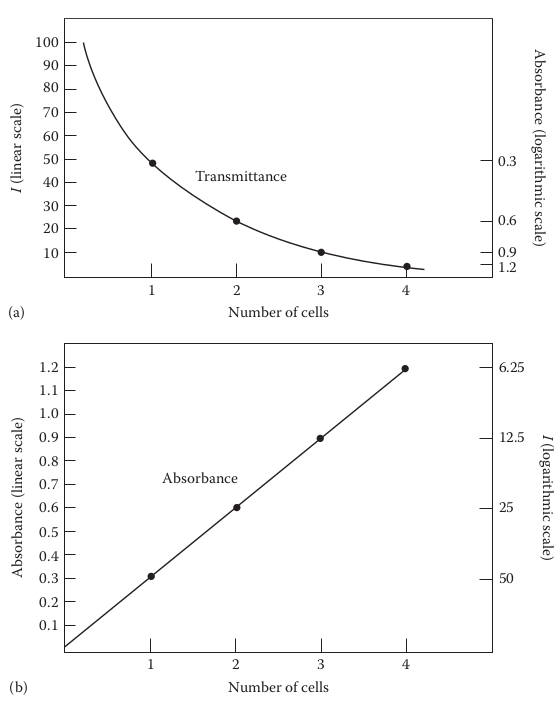
\includegraphics[width=0.85\textwidth]{2020-12-27_12-12.png}
        \caption{光程长对吸收的影响}
        \label{fig:2.10}
    \end{figure}
\end{problem}

保持光程长(样品池)不变,改变试样浓度,$I$、$A$与浓度之间的关系,与上例相同。
吸光度与浓度呈线性,于是我们得到
\begin{equation}
    A = \varepsilon l c
    \label{2.9}
\end{equation}
$l$是光程长度,单位为cm,$c$是样品浓度,单位为mol/L。$\varepsilon$是摩尔吸光
系数,对于给定物质,在特定波长下,该值为一常数。Beer在1852年发现浓度与吸光度
之间成正比关系。

综合吸光度、样品浓度、光程长度和摩尔吸光系数之间的关系,{\bf Beer-Lambert
-Bouguer}定律,简称为{\bf Beer}定律,从$A=-\log{T}$
\begin{equation}
    \varepsilon l c = -\log{T}
\end{equation}
\begin{equation}
    -\log{\left(\frac{I}{I_0}\right)}=\varepsilon l c 
\end{equation}
\begin{equation}
    \log{\left(\frac{I_0}{I}\right)}=\varepsilon l c 
\end{equation}
\begin{equation}
    \frac{I_0}{I}=10^{\varepsilon l c }
\end{equation}
\begin{equation}
    \frac{I}{I_0}=10^{-\varepsilon l c }
\end{equation}

根据观察到的实验事实,比尔定律从数学上表明,如果入射光的路径长度和波长保持
恒定,则$A$与吸收物质的浓度之间存在线性关系。这在分析光谱学中是极其重要的
关系。它通过定量测量吸收的辐射量,为定量分析样品中分析物的浓度奠定了基础。
辐射强度的定量测量称为光谱法。所有定量光学吸收光谱法(红外吸收光谱法,
AAS,UV/VIS吸收光谱法等)均满足比尔定律。
\subsection{Beer定律的偏差}
对于均质样品,通常在低分析物浓度下遵循Beer定律。当浓度小于约0.01 M时,大多数
吸收物质的吸光度与浓度成正比。

高浓度的分析物通常会出现线性偏差。在高浓度下有几种偏离线性的可能原因。
在溶液中浓度较低时,分析物将被视为溶质。随着溶质浓度的增加,分析物分子可能会
通过分子间吸引力(例如氢键和其他范德华力)开始相互影响。这种相互作用可能会改变
分析物的吸收率,从而随着浓度的增加而产生非线性响应。在极高的浓度下,溶质实际上
可能成为溶剂,从而改变了溶液的性质。如果分析物与其他物质处于化学平衡状态,
例如溶液中的弱酸或弱碱,则分析物浓度的变化可能会改变平衡(Le Chatelier原理)。
当溶液稀释或浓缩时,这可能反映在明显偏离比尔定律的地方。

如果样品散射入射辐射,则可能会出现另一种背离Beer定律的来源。溶液必须不含漂浮
的固体颗粒,并且在测量前通常要过滤。高分析物浓度时发生非线性的最常见原因是
光太少而无法吸收。在较低的分析物含量下,浓度加倍会使吸收的光量增加一倍,
例如从25\%增至50\%。如果已经吸收了99\%的光,则将浓度增加一倍仍将使吸收的剩余
光量增加一倍,但是变化仅从99\%到99.5\%。这导致曲线在高吸收率时变得平坦。

从式\ref{2.8}可以看出,$A = \log\left(I_0/I\right)$。如果$I_0 = 100$且
$A = 1.0$,则$I =10$。仅透射初始辐射强度的10\%。强度的其他90\%被样品吸收。
如果$A = 2.0$,则$I = 1.0$,表明99\%的入射光被样品吸收。如果$A = 3.0$,则
吸收99.9\%的入射光强度。正如我们将看到的,随着$A$的增加(或$I$的减少),$A$的
测量误差也随之增加。实际上,吸光度值小于或等于1.0符合Beer定律。
\section{数据处理方法}
建立我们测量的信号(例如吸光度)与已知分析物浓度之间关系。一旦建立了这种关系,
就可以通过测量未知信号来计算未知样品中分析物的浓度。随后讨论的方法不仅适用于
光谱测量,而且适用于大多数分析仪器方法。从历史上看,数据是通过手动读取仪表或
用直尺测量峰高,并将所有数字转录到实验室笔记本中来手动收集的。
信号和浓度之间的关系在座标纸上手动绘制。现代仪器具有软件包,这些软件包可以
使数据点统计到最适合的直线或曲线,并在计算机屏幕上显示结果并将其发送到打印机。
计算机化的数据收集和处理功能大大减少了抄写错误,将错误的图形复制到笔记本中。
线性回归和其他曲线拟合方法的使用,在拟合方程式和从方程式计算出的样品结果中
提供了更高的准确性和精确度。
\subsection{标准曲线法}
为了使用比尔定律确定未知物中的分析物浓度,必须确定给定波长下的吸光度与分析物
浓度之间的关系。已知浓度分析物的溶液称为标准溶液。对于某些类型的分析,标准液
可以采用固体或气体形式。

必须使用高纯度材料准确地制备标准品,以便尽可能准确地知道分析物的浓度。准备
涵盖适当浓度范围的一系列标准溶液。标准溶液应包括一种不添加分析物的溶液;该标准
溶液中分析物的浓度为零。该溶液称为试剂空白,用于解释由于溶剂和用于制备样品的
其他试剂中的杂质而引起的吸光度,它还说明了仪器基线。试剂空白和每种标准品的
吸光度为测量。在执行任何计算之前,将从其他标准溶液的吸光度中减去试剂空白
的吸光度。从中减去空白吸光度的吸光度称为“校正吸光度”。在$y$轴上校正吸光度
与$x$轴上标准品的已知浓度作图。这种图曾经在座标纸上手动构建;现在,绘图是由
计算机软件完成的。这种典型标准曲线如图\ref{fig:2.11}所示。该标准曲线显示了
IR区域中在石油中发现的正十六烷,\ce{CH3(CH2)14CH3}(在石油中发现的碳氢化合物)
在$3.41\mu m$处的吸光度与正十六烷在四氯乙烯,\ce{C2Cl4},中的溶液浓度之间的
关系。这种对正十六烷溶液在$3.41\mu m$处的吸光度的测量是一种用于确定水,土壤
和其他环境样品中石油污染的方法,因为大多数碳氢化合物都在该波长下吸收。依据
Beer定律来测量未知样品中的石油烃。它用于测量漏油,非法倒油和地下储油罐泄漏
造成的环境污染。
\begin{figure}[htpb]
    \centering
    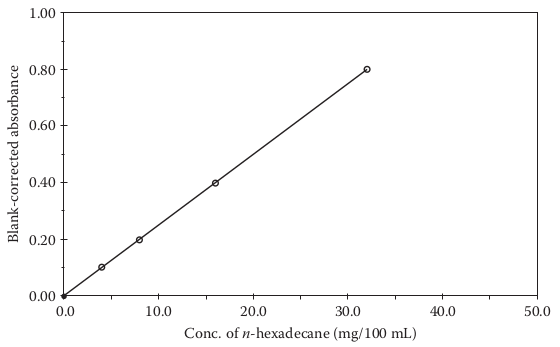
\includegraphics[width=0.75\textwidth]{2020-12-27_20-50.png}
    \caption{标准曲线示例}
    \label{fig:2.11}
\end{figure}
\begin{table}[htbp]
    \centering
    \caption{石油红外吸光度校正数据}
    \label{tab:2.4}
    \begin{tabular}{ccc}
        \hline
        正十六烷浓度 & $3.41\mu m$吸光度  &  修正吸光度\\
        \hline
        0.0  &  0.002   &  0.000  \\
        4.0  &  0.103   &  0.101  \\
        8.0  &  0.199   &  0.197  \\
        16.0  &  0.400   &  0.398  \\
        32.0  &  0.804   &  0.802  \\
        \hline
    \end{tabular}
\end{table}

表\ref{tab:2.4}给出每种标准品的浓度值以及测量和校正的吸光度。从图\ref{fig:2.11}
可以清楚地看出,此测量的吸光度与浓度之间的关系遵循比尔定律,因为该图产生一条
直线($y = mx + b$,其中$y$是吸光度,$x$是浓度)。绘制点后,将通过数据点
拟合最佳直线。最合适的直线拟合的方法是线性回归(线性最小二乘法)。当然,也可以
从标准曲线上直观观察到,与给定吸光度相对应的浓度。但为了进行精确工作,必须
确定最佳拟合直线方程式。

对表\ref{tab:2.4}中的数据进行拟合,可以得到确定的Beer定律关系式:
$A=0.0250 c - 0.001$,这里$c$是正十六烷的浓度,单位为mg/100 mL。根据标准曲线
方程,可以确定任何测量的吸光度的浓度。例如,根据美国EPA方法8440制备了未知的
受污染土壤样品,并测量样品溶液的吸光度为0.302,因此,修正后的吸光度为
$0.302 - 0.002 = 0.300$。从标准曲线中,我们可以观察到,这相当于12.0 mg
正十六烷/100 mL的浓度。精确的浓度可以通过线性回归方程计算得出,11.96 mg/100 mL
,或12.0 mg/100 mL(四舍五入三位有效数字)。

\begin{figure}[htpb]
    \centering
    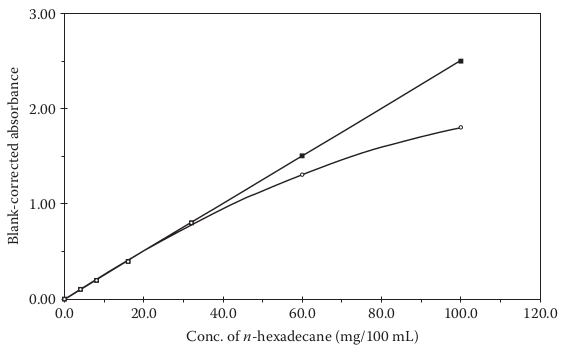
\includegraphics[width=0.85\textwidth]{2020-12-28_22-56.png}
    \caption{校正曲线}
    \label{fig:2.12}
\end{figure}
\begin{table}[htbp]
    \centering
    \caption{石油红外吸光度校正数据(高浓度)}
    \label{tab:2.5}
    \begin{tabular}{ccc}
        \hline
        正十六烷浓度 & $3.41\mu m$吸光度  &  修正吸光度\\
        \hline
        0.0  &  0.002   &  0.000  \\
        4.0  &  0.103   &  0.101  \\
        8.0  &  0.199   &  0.197  \\
        16.0  &  0.400   &  0.398  \\
        32.0  &  0.804   &  0.802  \\
        60.0  &  1.302   &  1.300  \\
        100.0  &  1.802   &  1.800  \\
        \hline
    \end{tabular}
\end{table}

假设除了表\ref{tab:2.4}列出的数据之外,我们还制备了正十六烷的标准溶液,其中包含
60.0 mg/100 mL和100.0 mg/100 mL两种浓度,吸光度数据如表\ref{tab:2.5}所示。
图\ref{fig:2.12}画出其它点,用空心圆表示,并标出了原始浓度。显然,在高浓度下,
偏离Beer定律,这些点不再是直线关系,测得的吸光度低于遵循Beer定律情况下的
吸光度。这说明,为什么将标准曲线外推延展到测量标准物的范围之外,从来不是一个
好主意。如果我们有一个吸光度为1.30的样品(60.0 mg/100 mL),并且使用我们原来
的标准曲线外推到更高的吸光度,图\ref{fig:2.12}黑色方块所示,那么我们将计算出
51.9 mg/100 mL的试样浓度,错误的降低了。如果吸光度高于最高 线性标准吸光度(
在此例中是$A=0.802$),最好的办法是将样品稀释。将60.0 mg/100 mL的样品进行稀释
十倍。
\subsection{标准加入法}
这种方法将已知量的分析物直接添加到样品中,其中包含未知量的分析物。由于添加
分析物而导致信号的增加(例如,吸光度,发射强度)使我们能够计算未知物中的
分析物量。为了使这种方法有效,分析物浓度和信号之间必须存在线性关系。

如果未准备好合适的外部校准曲线,则通常使用标准加入法。可能没有时间准备校准标准
品,例如,在医院紧急情况下,可能有必要快速测量患者血清中的钠。由于样品基质的
复杂性或缺少有关样品的足够信息,可能无法准备一套有效的校准标准。当流程中出现
问题时,行业通常需要分析``神秘''样本。当样品基质中存在某些类型的干扰时,非常有
用。 标准加入法允许我们通过在存在干扰的情况下执行校准来获得准确的结果,而不会
消除干扰。当仅需分析一个样品且外部标准品的制备效率低下时,通常会使用此方法。

标准加入法典型使用示例是通过原子发射光谱法测定未知成分的工业废水中的钠。提取
植物流的代表性样品,并分成四个等分试样,每个等分试样为100 mL。第一份等分试样
未经处理;这称为``不添加''或``零添加''样本。向第二等分试样中,以不明显改变体积
的方式向100 mL样品中添加100 $\mu$g \ce{Na}。这可以通过向样品中添加10 $\mu$L体积
的10000 ppm \ce{Na}溶液来完成。10000 ppm \ce{Na}溶液包含10000 $\mu$g \ce{Na}/mL
,因此下式所示,每10 $\mu$L部分包含100 $\mu$g \ce{Na}
\[
    \left(\frac{10000\quad \mu g\quad Na}{mL\quad solution}\right)
    \left(\frac{1\quad mL}{1000\quad \mu L}\right)
    \times 10\quad \mu L = 100\quad \mu g\quad Na
\]
现在第二个样品等分试样包含额外的1.0 ppm \ce{Na},因为100 $\mu$g \ce{Na}/100 mL
等于1.0 ppm \ce{Na}。向第三等分试样中,添加0.020 mL的10000 ppm \ce{Na}溶液;
现在,第三个包含额外的2.0 ppm \ce{Na}。在第四等分试样中,添加0.030 mL的10000
 ppm \ce{Na}溶液会在样品等分试样中产生额外的3.0 ppm \ce{Na}。由于添加了\ce{Na}
 溶液而引起的最大体积变化仅为0.03\%,数量可忽略不计。重要的是不要更改等分试样
 的体积,因为体积的变化会引起浓度-信号关系的变化。所有未处理的等分试样和
 已添加的等分试样必须具有相同的成分,否则标准加入法将不会产生准确的结果。
表\ref{tab:2.6}列出了添加的\ce{Na}的浓度和样品的等分试样编号。使用火焰俄歇
电子能谱(AES)或火焰光度计在589.0 nm的钠发射线上测量四个样品等分试样中
每一个的发射强度。测得的强度也列在表\ref{tab:2.6}中。此外,在没有样品的情况下
测量火焰的发射强度。这可测量“背景辐射”,即来自火焰的正信号,而不是样品引起的。
必须从样品强度中减去背景发射信号,就像我们前面所讨论的那样减去试剂空白,
才能获得表\ref{tab:2.6}中所示的校正强度。
 \begin{table}[htbp]
     \centering
     \caption{标准加入法}
     \label{tab:2.6}
     \begin{tabular}{lccc}
         \hline
         样品份 & 发射强度 & 修正强度  & \ce{Na}加入量(ppm)\\
         \hline
         1  &  2.9  & 2.4  &  0.0  \\
         2  &  4.2  & 3.7  &  1.0  \\
         3  &  5.5  & 5.0  &  2.0  \\
         4  &  6.8  & 6.3  &  3.0  \\
         背景  &  0.5  & 0.0  &    \\
         \hline
     \end{tabular}
 \end{table}
 \begin{figure}[htpb]
     \centering
     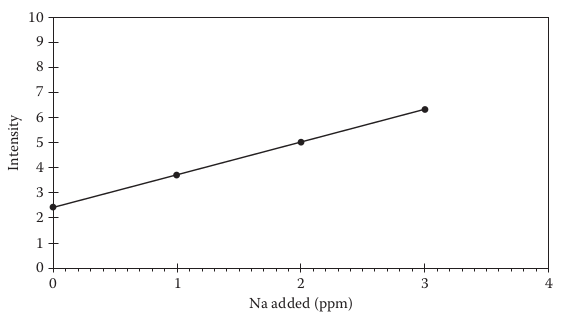
\includegraphics[width=0.85\textwidth]{2020-12-29_22-04.png}
     \caption{典型标准加入法曲线}
     \label{fig:2.13}
 \end{figure}

修正后的发射强度,相对于添加\ce{Na}浓度绘制曲线(图\ref{fig:2.13}。从图中可以
看出,所添加的浓度与信号之间的关系在所检测范围内,呈线性关系。
$\Delta I_{\text{emission}}/\Delta ppm \text{Na}$比值为斜率,通过线性回归
计算得出的。每1.0 ppm \ce{Na}加入,发射光强度增加1.3倍。未处理\ce{Na}样品浓度
的计算式为
\[
    \text{ppm Na} = \frac{R}{slope} = R(slope)^{-1}
\]
此处,$R$是第一份样品修正后的测量强度,$slope$为斜率。我们例子中,\ce{Na}
浓度为
\[
    \text{ppm Na}=2.4 \text{ initensity units}
    \times\frac{1.0 \text{ ppm Na}}{1.3 \text{ intensity units}}
    = 1.85 \text{ ppm}
\]
或者,可以使用确定的线性回归方程将标准加入曲线外推到$x$轴负方向上的截矩。样品
中\ce{Na}的浓度等于$x$轴截矩的绝对值。对于表\ref{tab:2.6}中数据,外推如图
\ref{fig:2.14}所示。$x$负方向截矩为$-18.5$;因此,样品中\ce{Na}的浓度为
$|-1.85 \text{ ppm}| = 1.85\text{ ppm}$
\begin{figure}[htpb]
    \centering
    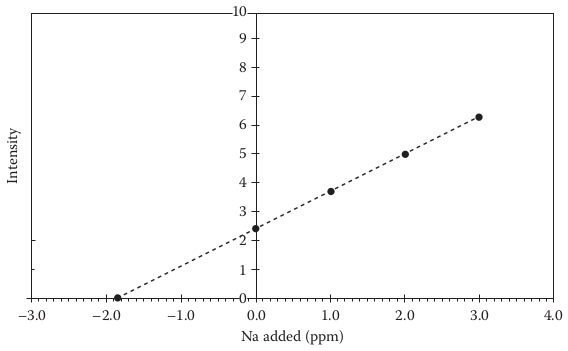
\includegraphics[width=0.85\textwidth]{2020-12-30_23-59.png}
    \caption{标准加入法}
    \label{fig:2.14}
\end{figure}
标准加入法是非常强大的工具,可在无法准备外部校准曲线时获得准确的分析结果。
在某些情况下,即使存在干扰物质的情况下,也可以获得准确的结果。此方法无法校正
背景发射或背景吸收或其他光谱干扰。

如果样品量有限(可能非常适合患者的血清),则可以使用单点标准添加技术。通过
火焰原子发射测定血清中钠的技术,测量样品的发射强度,然后添加已知浓度的\ce{Na},
而又不会明显改变样品的体积。测量添加样品的发射强度,以及火焰背景。发射信号与
浓度成正比,可以写成
\[
    \frac{I_{\text{unknown}}}{I_{\text{added}}} =
    \frac{\text{ppm Na}_{\text{unknown}}}
    {\text{ppm Na}_{\text{unknown}} + \text{ppm Na}_{\text{added}}}
\]
$I_{\text{unknown}}$是原始样品校正强度,$I_{\text{added}}$是添加\ce{Na}的样品
校正强度,$\text{ppm Na}_{\text{added}}$加入\ce{Na}的浓度。
例如,血清样品的测量给出2.4强度单位的校正强度。将足够的钠添加到血清样品中,使
浓度增加3.0 ppm,校正强度为6.3,设$x=\text{ppm Na}_{\text{unknown}}$,
\[
    \frac{3.7}{6.3}=\frac{x\text{ ppm}}{(x + 3.0)\text{ ppm}}
\]
解得
\[
    x = 4.3\text{ ppm Na}
\]
尽管样品有限,使用单点添加,可能的情况下至少两个添加,以确定分析方法的线性
范围。
\subsection{内标法}
内标法是添加到所有样品,空白和标准溶液中的已知量的非分析元素或化合物。
使用内标法进行校准是一种使用来自内部标准元素或化合物的信号来校正分析中干扰
的技术。通过内标法可以补偿多种误差源,从而提高分析的准确性和精确度。为确定
分析物A,选择样品中不存在的内标S。将相同浓度的S添加到所有样品,标准溶液和空白
样品中。测量归因于A和S的信号。计算归因于分析物A的信号与归因于内标S的信号的
比率。将信号比相对于标准液中的浓度比作图。通过线性回归可得到校准曲线的方程,
该方程应为线性以获得最佳结果。该公式允许通过测量样品中A和S的信号来计算
任何未知样品中的浓度比A/S,浓度与信号之间的关系可以表示如下:
\[
    \frac{\text{Concentration ratio(A/S) in sample}}
    {\text{Concentration ratio(A/S) in standard}} =
    \frac{\text{Signal ratio(A/S) in sample}}
    {\text{Signal ratio(A/S) in standard}}
\]
内标法广泛适用于光谱、色谱、质谱和其它仪器分析方法中。可以校正样品制备过程中
分析物的损失,分析过程中仪器中机械或电气的“漂移”,由于蒸发和其他类型的干扰
引起的体积变化。通常必须谨慎选择内标,以使内标的化学和物理行为与分析物相似。
内标不得与分析物发生化学和物理相互作用。任何影响分析物信号的因素,都应以
相同的方式影响内标物的信号。即使绝对信号发生变化,两个信号的比率也将保持
恒定。与不使用内标相比,这提供了更高的准确性和精确度。

通过电感耦合等离子体质谱仪(ICP-MS)对饮用水中的铅进行测定,内标如何纠正
诸如“仪器漂移”之类的问题,即一段时间内信号的变化。监视Pb-208同位素($^{208}$Pb
)的信号以确定铅。制备两种铅校准标样,每种标样均含10.0 ppb铅。一种标准品还
包含20.0 ppb的铋作为内标。\ce{Bi}信号与Pb-208信号一起在Bi-209同位素处测量。
一天中对这两种标准品进行了多次测量,结果信号列于表\ref{tab:2.7}。
从表\ref{tab:2.7}可以看出,
\ce{Pb}和\ce{Bi}的信号在一天中波动;例如,这种波动可能是由于仪器的电线电压
变化引起的。但是,如最后一栏所示,分析物信号与内标信号的比率在一天中保持恒定。
如果在上午8点不使用内标对ICP-MS进行校准,则在下午1点运行的样品会给出错误的
高Pb浓度,因为给定数量的铅的信号增加了2.5倍。在下午3点,样本将比真实值高大约
30\%。如果已将20.0 ppb \ce{Bi}添加到所有标准液和样品中,则Pb信号/Bi信号之比
将保持恒定,并确定准确的铅浓度。例如,ICP-MS在8 AM校准为仅含10.0 ppb \ce{Pb}的
标准溶液。对于10.0 ppb \ce{Pb},获得的信号为12050个计数。这是校准因子:
12050个计数/10.0 ppb铅。测量含有10.0 ppb \ce{Pb}和20.0 ppb \ce{Bi}的第二溶液;
如表\ref{tab:2.7}所示,铅的计数为12050(与标准值相同),而铋的计数为60000。
全天测量添加了20.0 ppb \ce{Bi}作为内标的饮用水样品。表\ref{tab:2.8}给出了
获得的信号。上午八点,铅信号为6028,没有内标物的情况下,使用校正因子计算水中
铅浓度
\begin{table}[htbp]
    \centering
    \caption{内标法校正}
    \label{tab:2.7}
    \begin{tabular}{lccc}
        \hline
        \multirow{2}*{测量时间} & 信号  &   信号  &  比率\\
        & 10 ppb Pb, m/e = 208 & 20 ppb Bi, m/e = 209 & Pb/Bi \\
        \hline
        上午八点 &  12050 & 60000  & 0.2008 \\
        上午十点 &  12100 & 60080  & 0.2013 \\
        下午一点 &  30000 & 149200  & 0.2010 \\
        下午三点 &  15750 & 78400  & 0.2009 \\
        \hline
    \end{tabular}
\end{table}
\[
    \begin{array}{rcl}
\text{ppb Pb in sample}&=&(6028)\dfrac{10.0\text{ ppb Pb}}{12050}\\
    \text{ppb Pb in sample}&=&5.00\text{ ppb Pb}
\end{array}
\]
这是样品中铅的真实值。使用相同方法,计算铅信号其余浓度,结果显示在表
\ref{tab:2.8}的第三列。下午一点和三点数据明显出现错误,归因于仪器“漂移”。
例如,下午一点的样品信号15010。使用铅校正因子计算浓度:
\[
    \begin{array}{rcl}
\text{ppb Pb in sample}&=&(15010)\dfrac{10.0\text{ ppb Pb}}{12050}\\
    \text{ppb Pb in sample}&=&12.5\text{ ppb Pb}
\end{array}
\]
仪器漂移的百分误差为:
\[
    \begin{array}{rcl}
    \text{\% Error}&=&\dfrac{\text{Measured value}-\text{True value}}
    {\text{True value}}\times 100 \\
    \text{\% Error}&=&\dfrac{12.5-5.00}{5.00}\times 100\\
    \text{\% Error}&=&+150\\
\end{array}
\]
如果使用内标\ce{Bi},内标校正因子,即Pb/Bi比率为:
\[
    10.0\text{ ppb Pb}=\dfrac{12050\text{ counts Pb}}{60000\text{ counts Bi}}
    =0.2008
\]
上午八点的样品,包含\ce{Bi}内标物,数据显示在表\ref{tab:2.8}。Pb/Bi比率为
$6028/60010=0.1004$,得到样品中铅浓度为:
\[
    \begin{array}{rcl}
        \text{ppb Pb in sample}&=&(0.1004)\dfrac{10.0\text{ ppb Pb}}{2.008}\\
        \text{ppb Pb in sample}&=&5.00\text{ ppb Pb}\\
    \end{array}
\]
\begin{table}[htbp]
    \centering
    \caption{有无内标水中铅的测定}
    \label{tab:2.8}
    \begin{tabular}{lccccr}
        \hline
        \multirow{2}*{测量时间} & \ce{Pb}计数 & ppb \ce{Pb} & \ce{Bi}计数 & 
        \multirow{2}*{Pb/Bi比率} & ppb \ce{Pb} \\
        & m/e = 208 & 无内标 & m/e = 209 & & 有内标 \\
        \hline
        上午八点 &  6028 & 5.00  & 60010 & 0.1004  & 5.00 \\
        上午十点 &  6063 & 5.03  & 60075 & 0.1009  & 5.02 \\
        下午一点 &  15010 & 12.5  & 149206 & 0.1006 & 5.01 \\
        下午三点 &  7789 & 6.46 & 78398  & 0.0994 & 4.95 \\
        平均值 &&7.25 &&&4.99\\
        标准差&&3.57&&&0.33\\
        相对标准差&&49.2&&&0.60\\
        真实值&&5.00&&&5.00\\
        误差&&45.0&&&$-0.2$\\
        \hline
    \end{tabular}
\end{table}
这与没有内标的结果相同。如果全天的样品内标的比率相同,仪器漂移的结果被修正。
例如,下午一点,\ce{Pb}为15010,\ce{Bi}为149206。这明显比上午八点高出很多,
但Pb/Bi的比率$15010/149206=0.1006$,铅的浓度为:
\[
    \begin{array}{rcl}
        \text{ppb Pb in sample}&=&(0.1006)\dfrac{10.0\text{ ppb Pb}}{2.008}\\
        \text{ppb Pb in sample}&=&5.01\text{ ppb Pb}\\
    \end{array}
\]
百分误差为:
\[
    \begin{array}{rcl}
        \text{\% Error}&=&\dfrac{5.01-5.00}{5.00}\times 100\\
        \text{\% Error}&=&0.2\\
\end{array}
\]
对于仪器分析来说,0.2\%的误差非常理想。

对比没有使用内标物的下午一点12.5 ppb的铅含量,尽可能的使用内标法是正确选择。
\subsection{Beer定律相关误差}
所有的光谱测量都有随机误差,直接影响准确度和精确度。光谱分析中最常见的随机
误差是仪器的“噪音”。噪音,归因于仪器光源的不稳定、检测器的不稳定、光路上样品
位置的变化,这些综合影响。误差是随机的,不能被消除。仪器辐射强度误差直接导致
使用校正曲线和Beer定律时浓度测量误差。

我们可以评估仪器噪音引起的随机误差对透过率测量的影响。以下讨论适用于光源强度
较低或检测器灵敏度较低的区域的UV/VIS和热检测器噪音较大的IR。根据Beer定律,
可以看出:
\begin{equation}
    \frac{\Delta c}{c} = \frac{0.434\Delta T}{T \log T}
    \label{2.15}
\end{equation}
其中,$\Delta c/c$浓度相对误差;$\Delta T$透过率测量误差。
\begin{definition}{推导过程}{beer}
\[
  -\log T = \varepsilon l c
\]
两边求导数
\[
  d(-\log T) = d(\varepsilon l c)
\]
等号左边$T$看作变量,右边$c$看作变量
\[
  -\frac{1}{x\ln 10}dT = \varepsilon l dc
\]
将$\varepsilon l = -\frac{\log T}{c}$代入,得
\[
  -4.303\frac{dT}{T} = -\log T \frac{dc}{c}
\]
\[
  \frac{\Delta c}{c} = \frac{4.303\Delta T}{T \log T}
\]
\end{definition}
可以从大量($n>20$)相同溶液的重复测量估算$\Delta T$的值。假设在$T$的测量中,
存在1\%的恒定误差,或者说$\Delta T=0.01$,可以使用式\ref{2.15}计算浓度的
相对误差,表\ref{tab:2.9}给出在该假定恒定误差下,各透过率测量中浓度的相对误差
。当$T$非常低或非常高的时候,浓度相对误差很大。当使用Beer定律,分析物的
浓度非常低(即透过率高),还是分析物浓度非常高(透过率低),都会导致重大误差。
\begin{table}[htbp]
    \centering
    \caption{相对浓度误差(1\%的仪器误差)}
    \label{tab:2.9}
    \begin{tabular}{lc}
        \hline
        透过率($T$) & 相对浓度误差($\Delta c/c$)$\times 100$(\%)\\
        \hline
        0.02 & 12.8\\
        0.08 & 4.9 \\
        0.15 & 3.5 \\
        0.30 & 2.8 \\
        0.37 & 2.7 \\
        0.45 & 2.8 \\
        0.65 & 3.6 \\
        0.80 & 5.6 \\
        0.97 & 33.8\\
        \hline
    \end{tabular}
\end{table}
\begin{figure}[htpb]
    \centering
    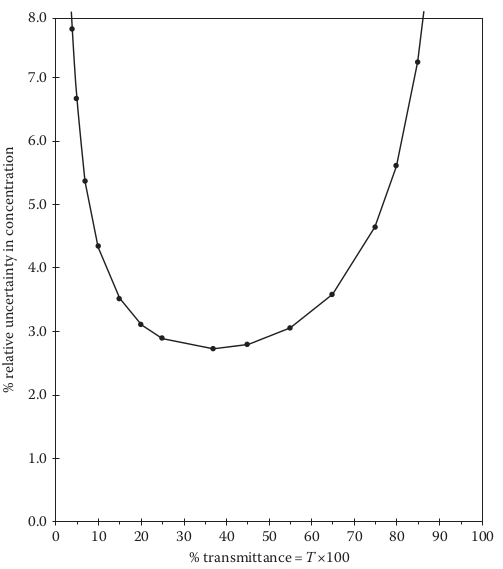
\includegraphics[width=0.75\textwidth]{2020-12-31_20-11.png}
    \caption{浓度测量的相对不确定性}
    \label{fig:2.15}
\end{figure}

我们可以将表\ref{tab:2.9}中的相对误差数据绘制为透过率的函数。结果如图
\ref{fig:2.15}所示。从该图可以看出,最小相对误差出现在$T = 0.37$,尽管
在15\%--65\%T的范围内可以获得令人满意的结果。该范围对应$于0.82 - 0.19$。为了
获得最大的定量吸收测量准确度,建议从吸光度在0.82至0.19之间的样品中确定浓度。
浓度过高的样品($A> 0.82$)应稀释以使其吸光度值低于0.8。太稀的样品
($A < 0.19$)应通过蒸发或溶剂萃取进行浓缩。如果无法更改样品溶液,分析人员
必须意识到,使用具有上述限制的仪器时,非常稀或非常浓的样品的相对误差会很大。

现代UV/VIS光谱仪通常受“shot noise”限制在光子检测器中电子穿越结。
在这种情况下,由于不确定的仪器误差而引起的相对不确定图与图\ref{fig:2.15}有
很大不同。对于高质量,shot noise受限的仪器,当A值非常低(\%T高)时,相对误差
会很高,但是从0.2到2.0以上的吸光度值具有大约相同的低($<1\%$)相对不确定度。
换句话说,由于仪器组件的改进,现代光谱仪比旧的光谱仪更加精确。

绘制光谱数据的另一种方法是使用Ringbom方法,其中横轴是浓度的对数,纵轴是
(100-%T)。所得的S形曲线称为Ringbom图。图\ref{fig:2.16}显示锰作为高锰酸根
离子吸收的Ringbom图。Ringbom图显示分析误差最小的浓度范围。这是曲线的陡峭部分,
斜率几乎是线性的。该图还可以评估在任何浓度水平下的准确度。根据Beer定律,可以
证明对于1\%的透射率误差,相对分析误差的百分比为
\begin{equation}
    \frac{\text{\% relative analysis error}}{\text{1\% transmittance error}} =
    \frac{100 \Delta c/c}{1} = \frac{230}{\Delta T/\Delta \log c}
    \label{2.16}
\end{equation}
因为数量($\Delta T/\Delta \log c$)是曲线的斜率,所以曲线上任意点每1\%的
透过率误差的相对分析误差等于230除以该点的斜率。可以通过在所需浓度下构建曲线的
切线来确定斜率。对于$x$的10倍差异,计算$y$的差异。该值除以230,即每1\%透射率
误差的相对分析误差百分比。例如,在图\ref{fig:2.16}中标记为A的两个点之间的斜率
是通过绘制切线来确定的,该切线穿过浓度2和20 ppm(变化10倍)。图中的$y$值在
2 ppm时为9\%,在20 ppm时为90\%。$y$值之差为$90 − 9 = 81$;因此,
$230/81 = 2.8$。在此范围内,相对分析误差为2.8\%。其他范围及其各自的误差在
图\ref{fig:2.16}左上方的插入框中显示。当然,与手动绘制切线相比,
使用计算机可以更准确地完成此计算。
\begin{figure}[htpb]
    \centering
    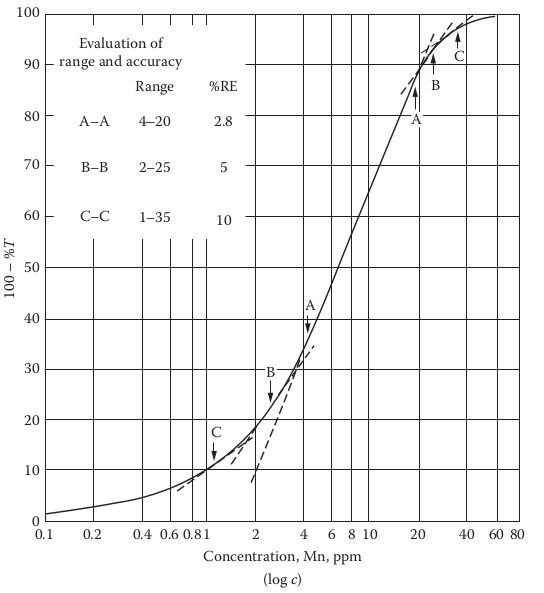
\includegraphics[width=0.75\textwidth]{2020-12-31_20-55.png}
    \caption{Ringbom图}
    \label{fig:2.16}
\end{figure}

Ringbom图的实际应用是确定浓度范围,在该范围内相对分析误差百分比不会超过指定值。
这种限制通常是为工业分析设置的,其中基于光谱测量结果为产品成分的上限和下限
建立了“好”产品的规格。超出这些规格的产品将被视为不符合要求而被拒绝。

对Ringbom图的解释得出的结论与我们从图\ref{fig:2.15}得出的结论相同。误差最低,
约为$100 - \% T = 63$或$37\% T$。每1\%透射率的相对分析误差约为2.8\%。在
40\%--80\%T或20\%至60\%T的范围内,误差不会显着增加;这是Ringbom图的陡峭,
近乎线性的部分。在纵轴的非常低和非常高的值下,Ringbom图的斜率接近零,因此,
相对光谱误差的百分比相对于光谱仪而言无穷大,而以前没有限制。

表\ref{tab:2.10}总结了光谱学中常用的术语,符号和定义。我们将在以后使用这些符号。
\begin{table}[htbp]
    \centering
    \caption{光谱学术语和定义}
    \label{tab:2.10}
    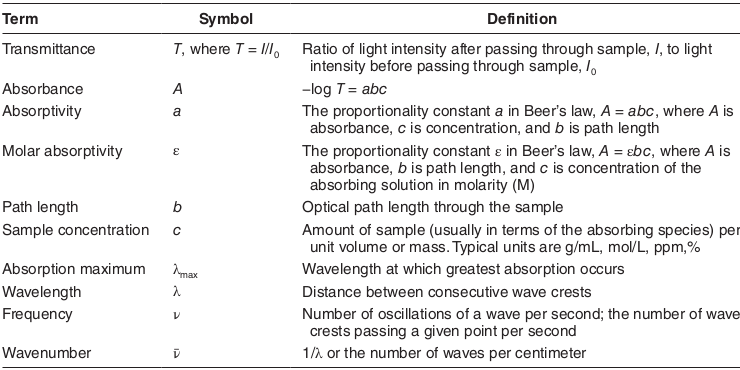
\includegraphics[width=0.9\textwidth]{2020-12-31_21-09.png}
\end{table}
\section{光学系统}
在光学分析光谱学中,测量样品对辐射的吸收或发射。用于测量辐射吸收或发射的仪器
必须提供有关吸收或发射的波长以及每个波长的强度(I)或吸收率(A)的信息。从光谱的
紫外到红外区域的光谱学研究仪器,其基本组成非常相似。目前,“光谱仪”将用于表示
用于光谱学的仪器。在讨论了组件之后,将为仪器定义更具体的术语。

用于分析光谱的仪器需要辐射源,波长选择设备(例如单色仪),对辐射范围透明的
样品架,用于检测辐射强度并将其转换为电信号的检测器,以及一些手段显示和处理
来自检测器的信号的过程。随后讨论的傅立叶变换(FT)光谱仪不需要波长选择设备。
如果要测量发射的辐射,则通过某种方式激发的样品就是辐射源。如果测量到光的吸收,
荧光,磷光或散射,则需要外部辐射源。这些组件的特定布置称为仪器的光学或光学配置
或光学布局。一个简单的单束吸收光谱仪的光学布局如图\ref{fig:2.17}所示。样品架和
波长选择器的放置可以颠倒;在UV/VIS吸收光谱法中,通常将样品架放置在波长选择器
之后,以使单色光落在样品上。对于原子吸收,红外和荧光光谱,通常将样品
放在波长选择器的前面。
\begin{figure}[htpb]
    \centering
    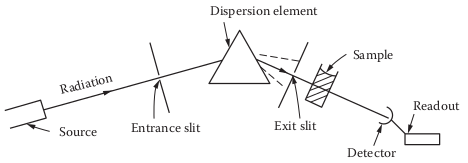
\includegraphics[width=0.75\textwidth]{2020-12-31_21-33.png}
    \caption{单束吸收光谱仪}
    \label{fig:2.17}
\end{figure}
\subsection{辐射源}
理想光谱辐射源应具备如下特征:
\begin{enumerate}
    \item 发射光必须涵盖所研究整个波长范围;
    \item 涵盖整个波长范围的辐射强度要足够高,可以避免来自检测器的信号放大;
    \item 光源在不同波长下,强度不应有明显变化;
    \item 光源强度不应随时间波动;
    \item 光源强度不应在短时间间隔内波动,这种波动称为“闪烁(flicker)”。
\end{enumerate}

辐射源的设计随其使用的波长范围而变化(例如,IR,UV,可见光),具体辐射源的详细
信息将在适当的仪器章节中进行讨论。大多数源的强度都会随电压的变化而呈指数变化,
因此在所有情况下,都需要向辐射源提供可靠,稳定的电源。电压调节器(也称为线路
调节器)可用来补偿输入电压的变化。如第2.6.5节所述,双光束光学配置也可用于补偿
光源稳定性的变化。

分析光谱中使用的辐射源有两种主要类型:连续体源和线源。连续谱源发出的辐射波长
范围很广,并且发射强度随波长的变化而缓慢变化。典型的连续体光源包括产生可见光
辐射(白光)的钨丝灯和高压氙弧灯,用于UV区的氘灯,用于UV区的高压汞或氙弧灯,
以及加热的固态陶瓷或光谱IR区域的加热线。连续谱源用于大多数分子吸收和荧光
光谱仪。相比之下,线源仅发射几个离散波长的光,强度是该波长的强函数。典型的线源
包括用于UV和可见光区域的中空阴极灯和无电放电灯,用于AAS和原子荧光光谱;用于UV
线的钠或汞蒸气灯(类似于现在在路灯中使用的灯)和可见光区域以及激光。激光是
高强度相干线光源;可提供在UV,可见光和IR区域具有发射线的激光。它们用作拉曼光谱
以及分子和原子荧光光谱中的来源。
\subsection{波长选择设备}
\subsubsection{滤波器}
选择电磁频谱某些部分的最简单、最便宜的方法是使用滤波器。有两种主要类型,吸收
滤波器和干涉滤波器。吸收滤光片可以像一块彩色玻璃一样简单。在第2.1节中,我们
讨论了蓝色玻璃如何透射可见光谱的蓝色波长,但吸收红色和黄色波长。这是用于
分离可见光谱的蓝色区域的吸收滤光器的示例。可以购买有色玻璃吸收滤光片,以隔离
各种范围的可见光。这些滤波器稳定,简单且便宜,因此非常适合用于便携式领域的
便携式光谱仪。最大的限制是与棱镜和光栅相比,透射的波长范围较宽。棱镜和光栅
也是用于从宽带多色光源中,选择较窄波长范围的设备。对于典型的吸收滤光片,透射
范围可能为50--300 nm。吸收滤光片仅限于光谱的可见光区域和X射线区域。

第二种类型的滤波器是干涉滤波器,由多层不同材料构成。该滤波器根据相长干涉原理
工作,以传输选定的波长范围。传输的波长由材料中心层的厚度和折射率控制。可以
构造干涉滤光片以透射光谱的IR,可见光和UV区域中的光。透射的波长范围比吸收滤光片
小得多,通常为1--10 nm,并且透射的光量通常比吸收滤光片高。
\subsubsection{单色器}
{\bf 单色器}由色散元件、入射狭缝和出射狭缝以及透镜和用于准直和聚焦辐射束的
反射镜组成。色散元件的功能是根据波长在空间中散射落在其上的辐射。两种最常见的
色散元件是棱镜和光栅。你可能已经很熟悉玻璃棱镜将白光分散为其组成
颜色的彩虹的功能。

入射狭缝允许来自光源的光落在色散元件上。分散的光落在单色器的出口狭缝上。出口
狭缝的功能是仅允许非常窄的光带穿过样品和检测器。实现此目的的一种方法是旋转
色散元件,以允许不同波长的色散光依次落在出口狭缝上。例如,白光源通过棱镜或光栅
,色散元件缓慢旋转,首先使紫色的光穿过出口狭缝,然后使蓝光等,一直到红光。
这样,单色器将来自光源的多色辐射分类为几乎单色的辐射,并离开出口狭缝。

\emph{棱镜}:棱镜用于分散IR、可见光和UV辐射。最常见的棱镜由用于紫外线区域的
石英,用于可见光和近红外(NIR)区域的硅酸盐玻璃,
\ce{NaCl}或\ce{KBr}用于IR区域。棱镜的形状像具有三角形横截面的条形。
$60^\circ–60^\circ–60^\circ$三角形(称为Cornu棱镜),如图\ref{fig:2.17}所示,
已被广泛使用,但也可以使用其他几何形状。穿过入口狭缝的多色光会聚在棱镜的一面上
,从而使入射光发生折射或弯曲。不同波长的光被折射到不同的程度,因此波长的空间
分离是可能的。棱镜材料的折射率随波长而变化。石英棱镜对短波辐射的折射率比
对长波辐射的折射率高;因此,短波辐射比长波辐射更易弯曲。如图\ref{fig:2.18}
所示,在光谱的可见区域中,通过这种棱镜时,红光的弯曲程度会小于蓝光。棱镜一直
以来是单色仪中最常用的分散设备,但已被衍射光栅或FT系统取代。
\begin{figure}[htpb]
    \centering
    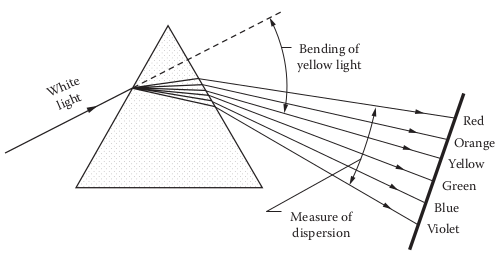
\includegraphics[width=0.65\textwidth]{2021-01-01_09-34.png}
    \caption{可见光通过棱镜色散}
    \label{fig:2.18}
\end{figure}

\emph{衍射光栅}:紫外线、可见光和IR辐射可以通过衍射光栅分散。衍射光栅由一系列
紧密间隔开的平行沟槽组成,这些沟槽被切成(或刻成)硬玻璃,金属或陶瓷表面
(图\ref{fig:2.19})。该表面可以是平坦的或凹入的,并且通常在直纹表面上涂覆
有反射涂层。用于紫外线和可见光区域的光栅将包含500至5000个凹槽/毫米,而用于
红外区域的光栅将具有50至200个凹槽/毫米。传统上,用金刚石工具对光栅中的凹槽
进行机械切割,这既费时又昂贵。这样的光栅被称为母版,并且用作从聚合物树脂浇铸
复制光栅的模具。复制光栅复制了原版中的凹槽,并涂有反射涂层,例如铝,以供使用。
大多数仪器使用复制光栅,因为它们比主光栅便宜得多。现在,大多数光栅都是通过
全息技术生产的。通过用光学平坦的光敏聚合物膜,涂覆光栅基板来制成光栅。
胶片暴露于激光束的干涉图样中,并且干涉图样被“燃烧”到胶片中。然后,使用化学或
离子蚀刻将干涉图案的凹槽蚀刻到基板中以制成主光栅,从而将凹槽成形为所需形状。
与机械刻划的主光栅相比,使用激光干涉图案形成凹槽可以以更低的成本获得更完美的
光栅。这些被称为全息光栅的光栅可以直接用于仪器中,也可以用作复制全息光栅
制造中的主光栅。全息光栅可以制成不同于传统平面或凹形的多种形状,并且根据应用,
凹槽的间距可以均匀或不均匀。典型的衍射光栅的尺寸在大约$25\times 25$到
$110\times 110$ mm之间变化。
\begin{figure}[htpb]
    \centering
    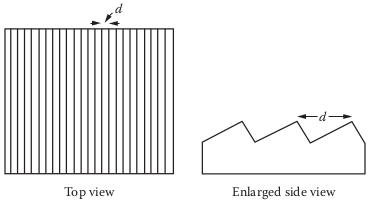
\includegraphics[width=0.65\textwidth]{2021-01-01_10-06.png}
    \caption{衍射光栅}
    \label{fig:2.19}
\end{figure}

光栅表面上的光分散是通过衍射发生的。反射光波之间的相长干涉,导致发生光衍射。
波的路径如图\ref{fig:2.20}所示。可以在相邻的凹槽上见到平行波。当发生
相长干涉或光衍射时
\begin{equation}
    n\lambda = d\left(\sin i \pm \sin\theta\right)
    \label{2.17}
\end{equation}
此处,$n$是光谱级次,其值可以取$1, 2, 3, \dots$整数;$\lambda$是入射光波长;
$d$是光栅相邻两刻痕间距离,称为光栅常数;$i$是光束入射角;$\theta$是波长
$\lambda$的光的散射角。
\begin{figure}[htpb]
    \centering
    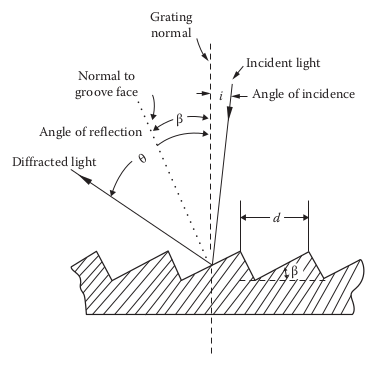
\includegraphics[width=0.65\textwidth]{2021-01-01_10-32.png}
    \caption{衍射光栅横截面:入射角$i$;衍射角$\theta$;光栅的闪耀角$\beta$;
    光栅间距$d$}
    \label{fig:2.20}
\end{figure}
入射角$i$和散射角$\theta$均从法线到光栅进行测量。$n$值一定,$\lambda$不同,
散射角不同。由于不同波长的光,以不同的角度衍射,发生光的分离。
\begin{figure}[htpb]
    \centering
    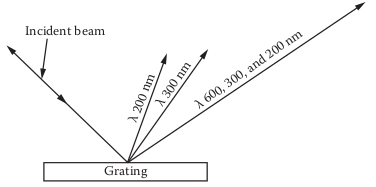
\includegraphics[width=0.65\textwidth]{2021-01-01_10-58.png}
    \caption{衍射角不但取决于波长,而且也取决于衍射级次$n$。波长为200、300
    300和600 nm的入射光,一阶($n=1$)不同的衍射角,但200 nm的三阶和300 nm的
二阶与600 nm的一阶重合}
\label{fig:2.21}
\end{figure}

光栅的一个问题是,几种不同波长的光可能以相同的色散角离开光栅。例如,假设
辐射束以角度$i$落在光栅上。对于给定的色散角$\theta$,根据公式\ref{2.17},
乘积$n\lambda$为常数。$n$和$\lambda$等于该常数的任何组合都将满足该方程式。
假设$\lambda = 600 nm$,$n = 1$给出了色散角$\theta$;那么,如果$\lambda=200 nm$
且$n = 3$,则角度也是$\theta$,依此类推。实际上,具有每个波长的辐射均以角度
$\theta$分散,并沿同一光路传播,如图\ref{fig:2.21}所示。以这种方式相关的光
的波长被称为衍射辐射的不同阶数。它们没有被光栅分开。色散后沿相同路径传播的
辐射的波长与数字$n$相关,该数字可以取任何整数的值。在高质量的光谱仪上,通过
使用小棱镜或滤光片系统作为与光栅结合的阶跃分选器,可以将不同阶分开
(图\ref{fig:2.22}和\ref{fig:2.23})。IR仪器通常将滤波器用作阶分类器。当光栅
旋转到不同的波长范围时,滤光片旋转以防止阶数重叠,并且只有一个波长到达检测器。
仪器公司Horiba Scientific(www.horiba.com)可以在Internet上找到有关衍射光栅和
光谱学的出色教程,方法是在主页上的搜索框中键入“光谱学教程”。
\begin{figure}[htpb]
    \centering
    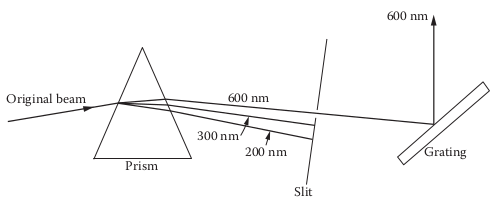
\includegraphics[width=0.75\textwidth]{2021-01-01_11-26.png}
    \caption{棱镜作为阶分类器}
    \label{fig:2.22}
\end{figure}
\begin{figure}[htpb]
    \centering
    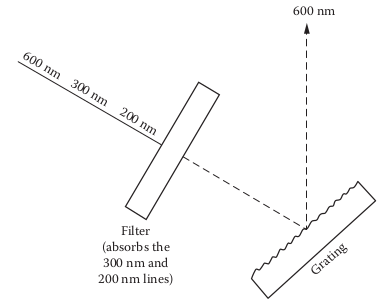
\includegraphics[width=0.65\textwidth]{2021-01-01_11-29.png}
    \caption{滤光片作为阶分类器}
    \label{fig:2.23}
\end{figure}
\subsubsection{分离两条不同波长所需的分辨率}
\emph{单色器波长精度}:在讨论系统分离两个波长的能力之前,评估系统的波长范围
非常重要。对于光谱的UV/VIS区域,可以通过扫描钬玻璃或钕镨玻璃,或市售的装有稳定
的高氯酸钬或高氯酸钕镨溶液的密封石英比色皿来完成。此类波长参考标准的一种来源
是Starna Cells,Inc.(www.starnacells.com)。如图\ref{fig:2.24}所示,这些化合物
会在整个UV/VIS区域产生一系列尖峰,应定期运行以确保从单色仪系统读取的波长准确。
可以使用类似类型的标准来检查远紫外和近红外区域的波长准确性。
\begin{figure}[htpb]
    \centering
    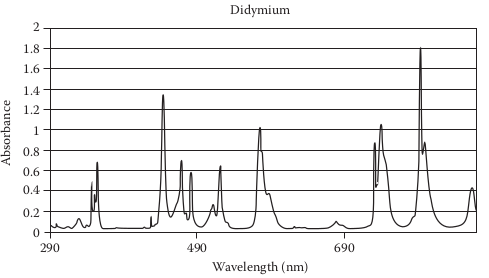
\includegraphics[width=0.85\textwidth]{2021-01-01_18-03.png}
    \caption{氧化钕镨UV/VIS波长参照光谱}
    \label{fig:2.24}
\end{figure}

\emph{单色器的分辨率}:分散辐射的能力称为分辨能力。替代名称包括色散功率和
分辨率。例如,为了观察599.9 nm的吸收带而不受600.1 nm的吸收带的干扰,我们必须
能够分辨或分离这两个带。

单色器的分辨能力$R$等于$\lambda /\delta\lambda$,其中$\lambda$是要分辨的两条线
的波长的平均值,而$\delta \lambda$是这两条线之间的波长差。在本示例中,
所需的分辨率为
\begin{equation}
    R=\frac{\lambda}{\delta\lambda}
    \label{2.18}
\end{equation}
\[
    R=\frac{\text{Average of 599.9 and 600.1}}
    {\text{Absolute difference between 599.9 and 600.1}}
    =\frac{600}{0.2}=3000
\]

\emph{棱镜的分辨率}:棱镜的分辨率$R$为
\begin{equation}
    R = t\frac{d\eta}{d\lambda}
    \label{2.19}
\end{equation}
此处,$t$是棱镜底部厚度;$d\eta/d\lambda$是棱镜材料的色散能力(或折射率)
$\eta$随波长的变化率。对于波长$\lambda_1$和$\lambda_2$的两个光束,棱镜的
折射率不相同。如果为常数,则不会发生分辨。棱镜的分辨能力随棱镜的厚度而增加。
通过选择棱镜材料,使$d\eta/d\lambda$最大,可以使给定波长区域的分辨率最大化。
例如,玻璃棱镜比石英棱镜更好的散射可见光。为了获得最大的色散,棱镜在接近于
不再透明的波长处最有效。
For maximum dispersion, a prism is most effective at wavelengths close to
the wavelengths at which it ceases to be transparent.
在更长的波长处,分辨率降低。

\emph{光栅分辨率}:光栅分辨率由下式给出
\begin{equation}
    R = nN
    \label{2.20}
\end{equation}
此处,$n$是级次(阶数);$N$是入口狭缝发出的光,照亮的光栅凹槽总数。因此,较长
的光栅,较小的凹槽间距,以及高阶数($n>1$)的使用会提高分辨率。假设我们可以
获得一个500/cm的光栅。一阶将589.5 nm和589.0 nm处的钠D线分开,需要多长光栅?
从式\ref{2.18}可知,所需分辨率$R$如下
\[
    R = \frac{589.25}{0.5}=1178.5
\]
光栅分辨率至少需要1179(四位有效数字)。但(光栅)$R=nN$,即$1179=nN$。由于
我们规定为一阶,$n=1$;因此,$N$所需凹槽总数,是1179。光栅每厘米包含500线。
于是,解得(1179/500),即2.358 cm。

另一种问法,每厘米多少凹槽,才能在3.00 cm内分辨出相同的钠D线(假设整个光栅都被
照亮)?需要1179的分辨率,对于一阶来说,总计需要凹槽数量为$nN=N=1179$,所以
\[
    N/cm = 1179/3.00 cm = 393 \text{lines/cm}
\]
不可能刻蚀出分数的凹槽,$N$必定为整数,计算结果取最接近整数。

实际中,通常测试苯蒸气来评估紫外线中的光栅单色器系统的分辨率,这会产生许多
紧密而尖锐的吸收线。市场上有售苯蒸气的密封石英池可用于评估。通常在几个带宽下
进行评估,如图\ref{fig:2.25}所示。
\begin{figure}[htpb]
    \centering
    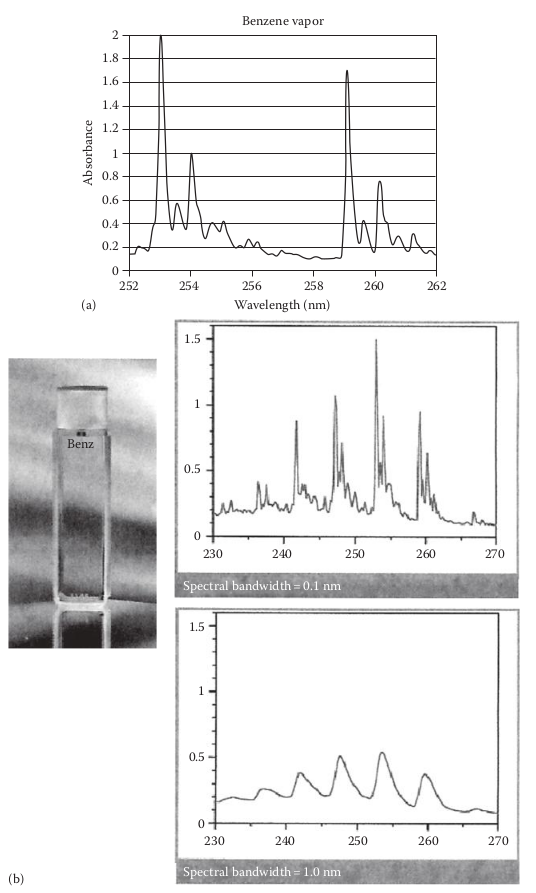
\includegraphics[width=0.85\textwidth]{2021-01-01_22-29.png}
    \caption{(a)苯蒸气光谱;(b)两种不同带宽下苯蒸气光谱}
    \label{fig:2.25}
\end{figure}

\emph{光栅单色器的色散}:衡量单色器分辨率的能力,就是看相邻波长的光是否能分开。
分辨率与倒数色散(或线性倒数)$D^{-1}$有关:
\begin{equation}
    D^{-1}=\frac{d\lambda}{dy}
    \label{2.21}
\end{equation}
线性色散的倒数等于波长的变化$d\lambda$与相应$y$的变化的比值,即,沿色散轴分割
波长的距离。$D^{-1}$的单位通常为nm/mm。$D^{-1}$作用在于,离开单色器的光的光谱
带宽(SBW)或光谱带通与$D^{-1}$和狭缝宽度直接相关:
\[
    \text{SBW}=sD^{-1}
\]
此处,$s$是单色器狭缝宽度。SBW表示离开单色器的光的75\%的波长范围的宽度。使用
光栅作为色散设备的单色器,线性色散倒数为
\begin{equation}
    D^{-1}=\frac{d}{nF}
    \label{2.23}
\end{equation}
$d$是光栅两个凹槽间距;$n$是衍射阶;$F$是单色器系统的焦距。因此,基于光栅的系统
相互色散在波长方面基本恒定。UV区域的SBW可以通过使用匹配的己烷中的溶液来确定。
在268.7 nm和267.0 nm处测量吸光度。计算吸光度比($A_{268.7}/A_{267.0}$),并与
SBW直接相关,如表\ref{tab:2.11}和图\ref{fig:2.26}所示。基于棱镜的单色器的色散
是更复杂的计算。
\begin{table}[htbp]
    \centering
    \caption{波长比率的带宽}
    \label{tab:2.11}
    \begin{tabular}{lccccr}
        \hline
        Ratio & 2.5 & 2.1 & 1.6 & 1.4 & 1.0 \\
        SWB   & 0.5 & 1.0 & 1.5 & 2.0 & 3.0 \\
        \hline
    \end{tabular}
\end{table}
\begin{figure}[htpb]
    \centering
    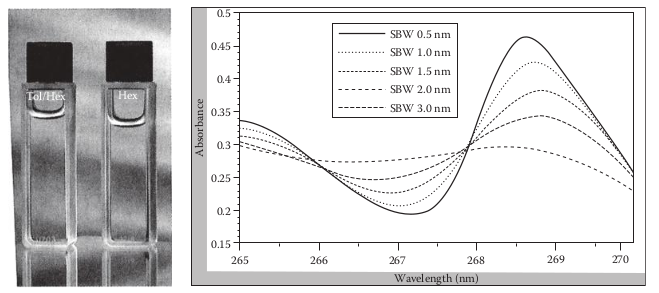
\includegraphics[width=0.85\textwidth]{2021-01-02_11-09.png}
    \caption{光谱带宽的测量(0.02\%甲苯的正己烷溶液)}
    \label{fig:2.26}
\end{figure}

\emph{Echelle单色器}:从图\ref{fig:2.19}和\ref{fig:2.20}可以看到,光栅表面上
显示的切口不是对称的$V$型。每个切口都有一个短面和一个长面。这种光栅称为闪耀
光栅(blazed grating)。如图\ref{fig:2.20}所示,常规的闪耀衍射光栅使用的凹槽的
长面,通常针对一阶衍射优化闪耀角$\beta$的切割角度。可以裁定具有更高闪耀角的
光栅,并可以使用凹槽的短面进行衍射;这种刮擦称为阶梯光栅。阶梯光栅的色散角
$\beta$比传统光栅高得多。echelle系统通过增加$\theta$角和使用更高阶(较大$n$
值)来改善色散。结果是,与相同焦距的常规光栅单色器相比,分辨率提高10倍。由于
衍射的多个高阶,因此有必要使用第二个分散元素对重叠的阶进行排序。第二个色散元件
,成为交叉色散器,用来对与光栅成直角的光进行分类,从而获得2D光谱。ICP发射光谱
(ICP-OES)的echelle光学布局如图\ref{fig:2.27}所示,图\ref{fig:2.28}显示2D
输出的示例,波长在$y$轴上绘制,衍射级在$x$轴。
\begin{figure}[htpb]
    \centering
    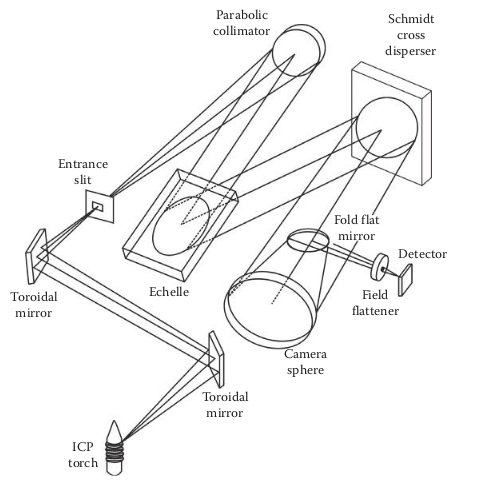
\includegraphics[width=0.75\textwidth]{2021-01-02_12-56.png}
    \caption{echelle光学布局}
    \label{fig:2.27}
\end{figure}
\begin{figure}[htpb]
    \centering
    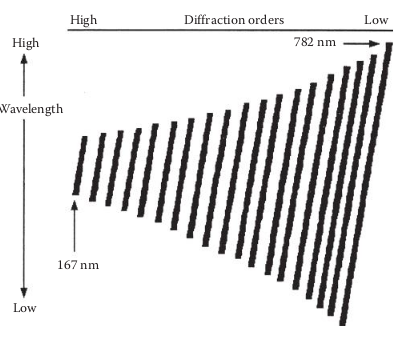
\includegraphics[width=0.75\textwidth]{2021-01-02_12-57.png}
    \caption{echelle光谱产生的色散2D阵列}
    \label{fig:2.28}
\end{figure}

\subsection{狭缝}
狭缝系统(图\ref{fig:2.17})用于从波长选择器分散光束之前和之后的光束中选择辐射
。狭缝的钳口由金属制成,通常形状像两个刀刃。它们可以彼此相对移动以根据需要改变
狭缝的机械宽度。为简单起见,图\ref{fig:2.17}并未显示单色器中用于根据需要
聚焦和准直光的透镜或反射镜系统。

入口狭缝允许来自光源的光束通过。来自光源的辐射聚焦在入口狭缝上。杂散辐射被排除
在外。通过入口狭缝后,辐射被准直成平行光束,该光束落在棱镜或整个光栅的一侧
并完全照亮。棱镜或光栅根据波长将光分散到不同的方向。在为色散设备选择的设置下,
将一个波长重新聚焦到出口狭缝上。其他波长的光也会聚焦,但不会聚焦到出口狭缝上。
发出的光线被重定向并聚焦到检测器上以进行强度测量。

透镜或前视镜用于聚焦和准直光。在红外中,前视镜总是比镜头更有效,并且不吸收辐射
。它们也很容易被刮擦,因为反射面在前部并且不受玻璃保护,就像常规镜子一样。
不使用背面镜,因为覆盖材料(例如玻璃)可能吸收辐射。图\ref{fig:2.29}显示了一种
类型的单色仪系统,该系统使用反射镜进行聚焦,准直,并使用光栅进行分散,
并显示了入口和出口狭缝。
\begin{figure}[htpb]
    \centering
    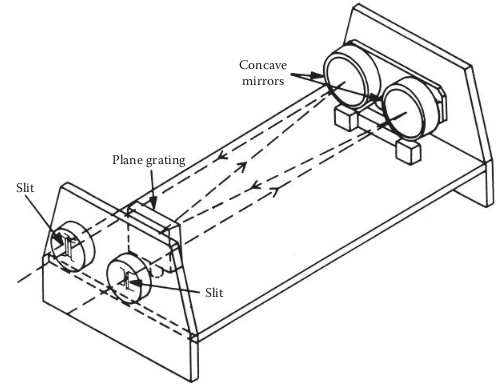
\includegraphics[width=0.85\textwidth]{2021-01-02_13-15.png}
    \caption{光栅单色器和狭缝}
    \label{fig:2.29}
\end{figure}

缝隙的钳口之间的物理距离称为机械缝隙宽度。以前装有千分尺的仪器,以便可以直接
读取机械狭缝的宽度;现代计算机控制的仪器通过控制运行狭缝机构的步进电机的软件
来设置和读取狭缝宽度。在紫外吸收光谱中,机械狭缝宽度约为0.3--4 $\mu m$。在红外
光谱中,色散仪器的缝隙宽度通常在0.1到2.0 mm之间。FTIR光谱仪中没有狭缝。

穿过出口狭缝的辐射的波长范围称为光谱带通或光谱带宽。如前所述,该带通可以通过
使用甲苯在己烷中的吸收光谱来测量。也可以通过将很窄宽度的发射线穿过狭缝到达
检测器来进行测量。通过旋转色散元件,我们可以记录发生响应的波长范围。校正发射线
的实际宽度后,我们可以计算光谱带通。例如,要测量用作AAS的单色仪系统的光谱带通,
我们可以使用镉空心阴极灯,它从镉产生非常窄的原子发射线。这些线之一出现在
228.8 nm。我们移动分散设备并在检测器上监视信号。镉的发射线在228.2至229.4 nm的
所有波长下发出信号。这意味着镉发射线在1.2 nm宽的波长范围内到达检测器。因此,
1.2 nm是此单色仪系统的光谱带通。在此示例中,未对228.8 nm镉线的实际宽度
进行校正,在这种情况下可以忽略不计。在上述实验中测量的信号具有高斯峰形状。
此类测量中的SBW通常定义为最大峰值高度的一半处的信号峰值宽度,称为半峰全宽
(FWHM)。光谱带通通常为0.3--4 nm。请注意,SBW比物理缝隙宽度(nm对$\mu$m)
小三个数量级。

如果机械狭缝的宽度变宽,则谱带通将同时增加,反之亦然。光谱带通是光谱仪中
影响分辨率的组件之一,如图\ref{fig:2.25}所示。例如,利用所描述的机械狭缝设置,
将不可能分辨出从228.8 nm \ce{Cd}线到229.0 nm处的发射线,因为两者都将穿过狭缝。
在实践中,缝隙应尽可能地窄以确保最佳分辨率。但是,它们必须足够宽,以允许检测器
测量足够的光。狭缝宽度的最终选择由分析师根据手头的特定样品确定。一个好的经验
法则是在不损害检测器功能或检测指定量分析物的能力的情况下,使缝隙尽可能窄。

通过旋转棱镜或光栅(或通过使出口狭缝横穿单色仪发出的光束),可以改变通过出口
狭缝的波长范围。通过将色散元件从一个极端连续旋转到另一个极端,
可以扫描整个光谱。
\subsection{检测器}
检测器用于测量落在其上的辐射强度。通常,它是通过将辐射能转换为电信号来实现的。
产生的能量通常很少,必须放大。来自检测器的信号必须稳定,并代表落在其上的
辐射强度。如果信号放大太多,它将变得不稳定,噪音多。信号中的随机变化程度称为
噪声级别。放大来自检测器的信号会增加其响应。在实践中,可以增加响应,直到信号
的噪声级别变得太大为止;否则,可能会增加响应。在这一点上,放大率降低,
直到噪声级别可以接受为止。

存在许多不同类型的光子检测器,包括光电倍增管、硅光电二极管、光伏电池以及
一类称为电荷转移设备的多通道检测器。电荷转移检测器包括光电二极管阵列、
电荷耦合器件(CCD)和电荷注入器件(CID)。这些检测器用于
原子/分子光谱学的UV/VIS和IR区域。

除光子探测器外,还有几个重要的探测器可以测量热量。这些热探测器在光子能量非常低
的IR区域特别有用。这些检测器将在以下各章中详细讨论特定技术,例如,IR检测器,
光电倍增管检测器和光电二极管、CCD和CID。
\subsection{单光束和双光束}
\begin{figure}[htpb]
    \centering
    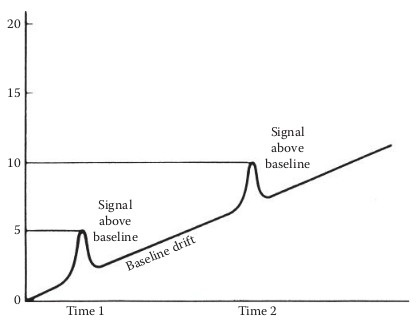
\includegraphics[width=0.85\textwidth]{2021-01-02_13-38.png}
    \caption{光谱测量中由于基线漂移导致的误差}
    \label{fig:2.30}
\end{figure}
如图\ref{fig:2.17}所示,单光束光学器件用于所有光谱发射方法。在发射过程中,将
样品放在图\ref{fig:2.17}中的源所在位置。在光谱吸收研究中,必须测量穿过样品
之前和之后的辐射强度。当使用单光束光学器件时,在进行测量时光源强度的任何变化
都可能导致分析误差。平均信号随时间的缓慢变化称为漂移,如图\ref{fig:2.30}所示。
漂移会导致所得结果直接错误。信号在时间0被设置为零,没有分析物存在。随着时间
朝着时间1增加,不存在分析物的信号(称为基线信号)由于漂移而增加。在时间1,由于
存在分析物(峰在基线上方显示),样品被测量并给出增加的信号。在时间1处的总信号
(样本加基线)为5个单位。基线继续向上漂移,在时间2,再次测量样品。从图中可以
看出,样品在基线以上的峰高与时间1的峰高相同,但是总信号(峰加基线)现在为10个
单位。如果不考虑基线漂移,分析人员将得出结论,时间2的样品分析物是时间1的两倍,
这是直接误差。

漂移的来源很多。辐射源强度可能由于线性电压的变化,源在最近打开后预热或源随时间
而改变。单色器可能会由于振动或加热和冷却而移动位置,从而导致膨胀和收缩。检测器
的线性电压可能会发生变化,或者检测器可能会随着时间而变差并导致响应发生变化。
与校准中使用的标准相比,由漂移引起的误差会导致发射信号或吸收信号的测量误差。
通过不断检查光强度或使用分析过程中以频繁间隔测量的标准溶液,可以减少此问题。
单光束光学器件尤其容易受到漂移引起的误差的影响。但是,通过使用双光束系统
可以大大减少与漂移相关的问题。

\begin{figure}[htpb]
    \centering
    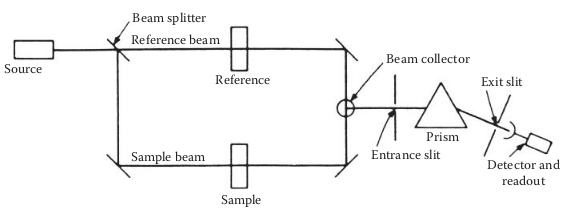
\includegraphics[width=0.85\textwidth]{2021-01-02_15-11.png}
    \caption{双光路系统}
    \label{fig:2.31}
\end{figure}

双光束系统广泛用于光谱吸收研究。系统的各个组件与单光束系统具有相同的功能,
但有一个非常重要的区别。使用分束器将来自源的辐射分成强度近似相等的两束光束,
如图\ref{fig:2.31}所示。一束称为参考束;穿过样品的第二束称为样品束。然后将两个
光束重新组合,并通过单色器和狭缝系统到达检测器。图\ref{fig:2.31}对此进行示意性
说明。在此示意图中,参考光束中有一个单元与用于保存样品的单元相同。例如,参比池
可以是空的,也可以包含用于稀释样品的溶剂。样品后显示单色器的这种特殊安排是
分散IR双光束分光光度计的典型特征。双光束系统的光学布局有许多商业上的变化。

\begin{figure}[htpb]
    \centering
    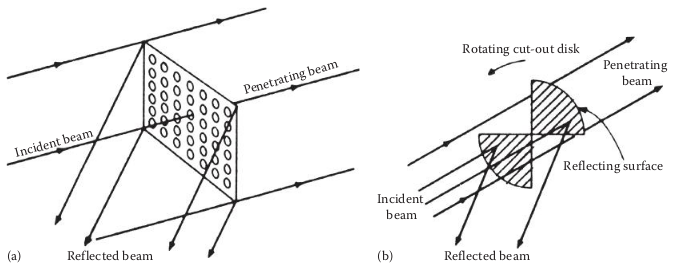
\includegraphics[width=0.85\textwidth]{2021-01-02_15-13.png}
    \caption{(a)板式分束器;(b)旋转分束器}
    \label{fig:2.32}
\end{figure}
\begin{figure}[htpb]
    \centering
    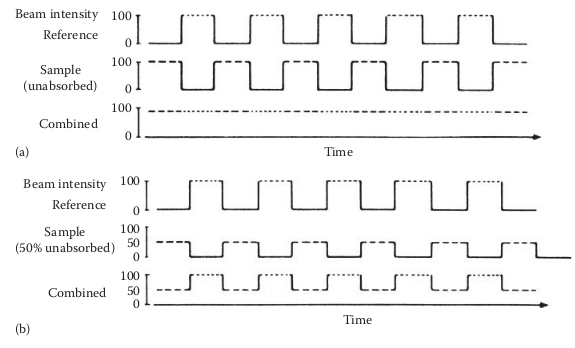
\includegraphics[width=0.85\textwidth]{2021-01-02_15-15.png}
    \caption{经过旋转分束器达到检测器的辐射强度:(a)没有吸收;(b)吸收50\%}
    \label{fig:2.33}
\end{figure}

如图\ref{fig:2.32}(a)所示,分束器可以是一个简单的镜板,在其中钻有许多孔。光被
镜板反射并向下穿过样品光束路径。相等的一部分光穿过板上的孔并形成参考光束。
另一个方便的分束器是去除相对象限的盘(图\ref{fig:2.32}(b))。圆盘在辐射束的前面
旋转,镜面将光反射到样品路径中。丢失象限允许辐射沿参考路径通过。每束光束都是
断续的,并以交变信号的形式到达检测器。当样品没有吸收任何辐射时,两个光束相等,
重新结合并形成稳定的光束。但是,当辐射被样品吸收时,两个光束不相等,并且交替
信号到达检测器。如图\ref{fig:2.33}所示。

使用双光束系统,我们可以测量参考光束强度与样本光束强度的比率。因为使用了比率,
所以在测量过程中来自源的辐射强度的任何变化都不会引起分析误差。这一优势彻底
改变了吸收光谱。如果信号中存在漂移,则它会同样影响样本和参考光束。除非漂移非常
大,否则重组光束将继续提供准确的信号信息,在这种情况下,校正不会完成。使用
双光束系统进行的吸收测量实际上与漂移无关,因此更准确。
\subsection{傅立叶变换光谱仪}
前述的色散光谱系统将光分成其分量波长,并将其传播到光谱中。在这些系统中,可以
沿着波长与位置成比例的路径在每个点处测量强度。可以通过缓慢移动光栅来确定光谱中
每个点周围狭窄区域的强度,以使分散光谱的每个区域都通过单个固定检测器。或者,
系统可以使用连续的检测器阵列同时测量所有波长区域。后一种方法可在更少的时间内
获取更多信息。它可以通过使用一维光电二极管阵列或2D CCD在UV/VIS区域中实现,这与
现代数码相机中的类似。

能量较低的红外波长的检测器无法轻易小型化,因此色散红外采用慢扫描方法工作。为了
使用扫描仪器获得高波长分辨率,需要将到达检测器的波长区域限制在非常窄的窗口内。
反过来,这需要缓慢扫描光谱以达到所需的灵敏度。

FT光谱仪采用的光谱采集方法与色散系统中使用的光谱采集方法截然不同。理想的是同时
测量所有波长的光,其方式应允许强度与波长曲线(即光谱)的重建。如果波长信息
以明确定义的方式编码,例如通过使用干涉仪对光强度进行调制,则数学方法可以将信息
解释和呈现为从色散仪器获得的相同类型的光谱。在没有分散设备的情况下执行此操作
的仪器称为多路复用仪器。如果同时收集所有感兴趣的波长而不分散,则这些波长及其
相应的强度将重叠。必须对产生的重叠信息进行分类以绘制频谱。排序或“解卷积”变化
频率(或波长)的重叠信号的常用方法是一种称为傅立叶分析的数学程序。此处介绍的
示例是IR光谱学,它是仪器分析化学中的第一个应用程序,但是该原理还与其他技术结合
使用,在这些技术中,分析数据显示为响应随频率变化的频谱,例如NMR和离子回旋
共振MS。

傅里叶分析允许将任何连续曲线(例如,强度峰和谷的复杂光谱作为波长或频率的函数)
表示为随时间变化的正弦或余弦波之和。相反,如果可以将这些正弦波和余弦波的等效值
作为数据来获取,则可以将其进行傅立叶变换成频谱曲线。这就要求以数字形式进行数据
采集,强大的计算能力和高效的软件算法,而这些功能现在已经可以在当前的
个人计算机,笔记本电脑和手持设备的级别上轻松获得。例如,采用这种方法的计算机
化仪器称为FT光谱仪-FTIR,FTNMR和傅里叶变换质谱(FTMS)仪器。

FT光谱仪使用的干涉仪在设计上类似于图\ref{fig:2.34}所示的迈克尔逊干涉仪。为了
简化讨论,我们首先考虑产生波长为$\lambda$的单色辐射的光源。源辐射射到分束器上,
分束器将一半的光透射到固定镜,其余的反射到移动镜。可以对移动镜进行编程,使其
以精确控制的恒定速度沿光束路径移动。光束从镜子反射回分束器。每束光线的一半直接
穿过样品架到达检测器。其他两半沿源的方向向后移动,无需进一步考虑。如果固定镜和
移动镜与分束器的距离完全相等,则两个半光束将同相合并。组合波的振幅将是每个半波
的两倍,并且检测器信号将达到最大。如果移动镜随后移动等于$\lambda / 4$的距离,
则两个半光束将异相合并180$^\circ$(即$\lambda/ 2$)。光束产生相消干涉,检测器
未记录任何信号。对于反射镜之间的路径差的所有其他值,会发生部分相消干涉。当移动
镜以恒定速度移动时,到达检测器的信号会通过这种相长和相消干涉的重复模式有规律地
循环。当路径差$\delta$是$\lambda$的整数倍时,它最大化;当$\delta$是$\lambda$的
半整数倍时,它变为零。在FTIR中,$\delta$称为延迟。对于单色光,信号(功率,
强度)与$\delta$的关系图称为干涉图,其形式为简单的纯余弦曲线:
\begin{equation}
    P(\delta)=B(\bar{u})\cos(2\pi\delta\bar{u})
    \label{2.24}
\end{equation}
$P(\delta)$是达到检测器喜好的幅度;$B(\bar{u})$是一个与频率相关的常数,说明仪器
的变量,例如检测器响应,分束器投射或反射的光量以及光源强度。
波数$\bar{u}$等于$1/\lambda$。干涉图是到达检测器的干扰信号的记录。它实际上是
一个“时域”频谱。它记录检测器响应随时间变化的方式。如果样品吸收特定频率的光,
则该频率的幅度会发生变化。对于连续光源(在感兴趣区域内所有波长的输出具有连续
可变输出的光源),干涉图是一条复杂曲线,可以表示为无穷余弦波和反射光吸收的
不同幅度的总和通过样本。尽管很复杂,但是如果在足够数量的点处对干涉图进行采样,
则使用快速傅里叶变换(FFT)的现代计算机可以处理干涉图并识别足够的余弦波,从而
可以将数据解卷积为强度的IR光谱图与波长的关系。
\begin{figure}[htpb]
    \centering
    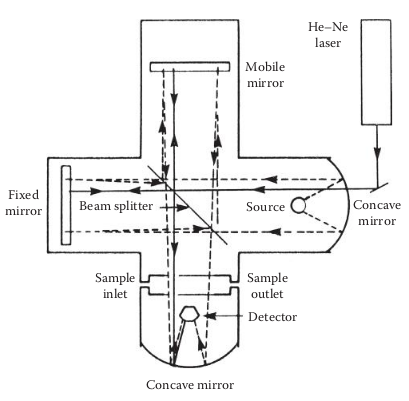
\includegraphics[width=0.85\textwidth]{2021-01-02_16-43.png}
    \caption{FTIR光谱仪}
    \label{fig:2.34}
\end{figure}
\subsubsection{傅立叶系统的优点}
与分散系统相比,FT光谱仪产生更好的信噪比。这是由几个因素造成的。 FT仪器的光学
元件较少且没有狭缝,因此到达检测器的辐射强度比色散仪器高得多。信号的增加会增加
信噪比。这称为吞吐量优势或雅奎诺特优势。同时测量所有可用波长,因此大大减少了
收集所有数据以形成光谱所需的时间。整个红外光谱可以在不到1秒的时间内收集到。这
使得实用的频谱测量的数百次重复的收集和信号平均化成为可能。信号平均对S/N的理论
改进与平均频谱数$(n)^{1/2}$的平方根成正比。这种优势称为多路复用或Fellgett优势。

FT光谱仪具有很高的波长重现性。在FTIR光谱仪中,移动镜在移动过程中的位置通过
光学系统使用来自可见范围激光器的高度单色光的平行干涉测量法以极高的精度连续进行
校准,如图\ref{fig:2.34}所示。在干涉图进行傅立叶变换之后,这种精确的位置测量
结果可以转换为准确且可重现的分析波长测量结果。这种精确的位置测量可以精确地
添加多个光谱,从而获得多重优势。

应该注意的是,FT光谱仪是单光束仪器。背景必须与样品光谱分开收集。这两个光谱的
比率导致背景校正的光谱,类似于从双光束仪器获得的光谱。尽管不能同时采集样品和
背景光谱,但由于可以快速采集和快速处理光谱,因此可以定期采集背景光谱,以避免
单光束色散仪遇到的问题。
\section{光谱技术和仪器命名}
光谱学和光谱仪器已经发展了许多年。毫无疑问,所使用的术语也已经发展并且实际上
正在不断发展。科学术语通常是由专业组织定义的,有时这些组织在定义上不一致,从而
导致使用同一术语来表示不同的含义。科学家(和学生)必须及时了解术语的含义以进行
有效的交流,但还必须了解术语的较旧用法才能理解文献。光谱学一词是指研究电磁辐射
与物质的相互作用。术语“光谱法”用于定量测量一个或多个电磁辐射波长的强度。分光
光度法是保留用于吸收测量的术语,其中必须在双光束系统中同时测量或在单光束系统中
依次测量两种强度(样品和参考)的比率。该术语逐渐被光谱学取代;例如,atomic
absorption spectrometry比atomic absoption spectrophotometry更普遍。

用于仪器的术语通常区分如何选择波长或使用的检测器类型。光谱仪是一种由棱镜或光栅
色散装置,狭缝和光电检测器组成的仪器,用于测量透射率或吸收率。但是,术语
“光谱仪”现在也适用于非分散且没有狭缝的基于IR干涉仪的FT系统。分光光度计是指
双光束光谱仪;但是,该术语现在同时用于吸收测量的单光束和双光束色散光谱仪。
光度计是一种光谱仪,它使用滤光片来选择波长而不是色散装置。光谱仪是一种具有
分散装置的仪器,该仪器具有较大的孔径而不是微小的出口狭缝,并且使用照相胶片进行
检测(现已淘汰)或使用固态成像检测器。
\newpage
\section{实验练习}
\begin{exercise}\label{exer:1.1}
UV/VIS光谱仪、样品池等。
\begin{enumerate}[a.]
\item 制备标准溶液:(1)0.1 g/L \ce{KMnO4}水溶液;(2)1.0 g/L \ce{K2Cr2O7}水溶液
    ;(3)用水稀释50\%的红墨水溶液。
\item 在350--700 nm范围内检测三种溶液的最大吸收波长。
\item 计算三种溶液最大吸收波长处的透射率$I/I_0$。
\end{enumerate}
\end{exercise}
\begin{exercise}
\begin{enumerate}[a.]
\item 练习\ref{exer:1.1}(a)中选择一种标准溶液(标记为A),测试最大吸收处的透射
    率。取50 mL至100 mL容量瓶中,去离子水定容(标记为B)。测量和记录溶液B的透射
    率。取50 mL溶液B,定容于100 mL容量瓶中(标记为C),测量和记录溶液C的透射率
    。如此类推,溶液D、E和F。
\item 以A到F的数据,拟合、绘制透射率-浓度曲线。
\item 计算每种溶液的吸光度,并拟合、绘制吸光度-浓度曲线。
\item 计算未知浓度溶液,使用那张图更合适一些?为什么?
\end{enumerate}
\end{exercise}
\begin{exercise}
\begin{enumerate}[a.]
\item 取练习\ref{exer:1.1}配置\ce{KMnO4}溶液10.0 mL,并加入该练习配置的
    \ce{K2Cr2O7}溶液10.0 mL,混合后,测量吸收。
\item 取10.0 mL\ce{K2Cr2O7}溶液加到10.0 mL去离子水中,并测量吸收。
\item 取10.0 mL\ce{KMnO4}溶液加到10.0 mL去离子水中,并测量吸收。使用每种化合物
    最大吸收波长,回答下面问题。与包含单一化合物的溶液相比,包含两种化合物的
    溶液最大吸收波长处的吸光度有没有变化?单一溶液吸收的光总量等于混合物吸收
    光量之和吗?吸光度的这种变化(如果有的话)会导致误差吗?误差是正还是负?
    如果必须测量\ce{KMnO4}和\ce{K2Cr2O7}混合物,你能想到纠正此误差的方法吗?
\end{enumerate}
\end{exercise}
\begin{exercise}
在其最大吸收波长下,测量新鲜制备的\ce{KMnO4}水溶液的吸收率。溶液的浓度应使
吸光度约为0.6--0.8。将溶液放入容量瓶中,然后将溶液直接从容量瓶中倒入样品架中
进行首次测量。现在,将溶液从烧瓶中倒入烧杯或宽口广口瓶中(您要使表面积最大化)
。让溶液在大气中暴露5分钟,然后再次测量溶液的吸光度。每隔5分钟重复一次测量。
(如果看不到变化,则将样品盖好并摇匀,然后解开盖,使其在空气中静置。)相对于
暴露在空气中的时间绘制测得的吸光度。这种变化是由\ce{KMnO4}的化学不稳定(它与
空气反应)引起的。如果将其用作校准的标准解决方案,则此更改将导致错误。许多标准
解决方案或多或少都会受到此类错误的影响,因此必须采取预防措施来防止和避免这种
麻烦。建议使用两种方法来避免\ce{KMnO4}出现此问题。
\end{exercise}
\newpage
\begin{problemset}
\item 分子吸收频率为$3.00\times 10^{14} Hz$的辐射,两个能级差是多少?
\item 波长为$500.0 nm$的辐射,频率是多少?
\item 描述原子吸收UV辐射所发生的跃迁。
\item 按波长递增的顺序排列:IR, radiowaves, X-rays, UV, visible light。
\item 对于给定的跃迁,原子或分子的吸收程度是否取决于基态或激发态的数量?为什么?
\item 对于给定的跃迁,云子或分子的发射程度是否取决于基态或激发态的数量?为什么?
\item 简要描述大多数分子中发生的三种跃迁类型,和跃迁中所涉及的辐射类型。
\item 简述Beer-Lambert-Bouguer定律的数学公式,并解释等式每个符合的含义。
\item (a)定义透射率和吸光度;(b)浓度与(1)透射率(2)吸光度之间有什么关系?
\item 使用图2.16,通过将线延长到覆盖浓度差异的10倍,来计算通过标记为B的较低点
    绘制切线的斜率。通过找到曲线上部分的斜率等于刚计算出的斜率,来确认相对误差
    为1\%(\% RE)的B--B所示范围是正确的。重复计算C点并确认C--C范围。
\item 通过在$510 nm$和$1.00 cm$光路下测量反应\ce{Fe^2+}与1,10-菲啰啉红色络合物
    溶液的透射率,在用于铁含量测定的外标校准中获得以下数据
    \begin{table}[htbp]
        \centering
        \begin{tabular}{llll}
            \hline
            铁浓度(ppm)&透射率(\% T)&铁浓度(ppm)&透射率(\% T)\\
            \hline
            0.20 & 90.0 & 3.00 & 26.3 \\
            0.40 & 82.5 & 4.00 & 17.0 \\
            0.60 & 76.0 & 5.00 & 10.9 \\
            0.80 & 69.5 & 6.00 & 7.0 \\
            2.00 & 41.0 & 7.00 & 4.5 \\
            \hline
        \end{tabular}
    \end{table}

    (a)计算每种溶液的吸光度$A$,并绘制吸光度-铁浓度曲线(你可以使用电子表格
    程序)。
    系统在整个浓度范围内是否符合Beer定律?(b)计算平均摩尔吸光系数;(c)绘制
    透射率(100--\% T)相对于浓度对数曲线图(Ringbom法),(1)在此范围内最佳浓度
    范围和最大准确度是多少?(每1\%透射率误差的\%RE)(2)在什么浓度范围内,每
    1\%透射率误差的相对分析误差不超过5\%?
\item 下表是标准曲线法测定铜(\ce{Cu(NH3)4^2+})数据
    \begin{table}[htbp]
        \centering
        \begin{tabular}{llll}
            \hline
            铜浓度(ppm)&透射率(\% T)&铜浓度(ppm)&透射率(\% T)\\
            \hline
            0.020 & 96.0 & 0.800 & 27.8 \\
            0.050 & 90.6 & 1.00 & 23.2 \\
            0.080 & 84.7 & 1.40 & 17.2 \\
            0.100 & 81.4 & 2.00 & 12.9 \\
            0.200 & 66.7 & 3.00 & 9.7 \\
            0.400 & 47.3 & 4.00 & 8.1 \\
            0.600 & 35.8 &  &  \\
            \hline
        \end{tabular}
    \end{table}

    计算每一溶液的吸光度,绘制吸光度--铜浓度曲线。在这些条件下,进行测量的系统
    在整个浓度范围内是否符合Beer定律?是否有小量的或大量的定律偏离?提出任何
    可能的偏差产生原因。
\item 将$0.200 g$铜溶于硝酸中,加入过量的氨生成\ce{Cu(NH3)4^2+},定容至1 L。
    分别取该溶液10.0, 8.0, 5.0, 4.0, 3.0, 2.0和1.0 mL,并定容于10.0 mL。对应的
    吸光度分别为0.500, 0.400, 0.250, 0.200, 0.150, 0.100和0.050。通过形成
    \ce{Cu(NH3)4^2+}络合物并测量吸光度来分析一系列样品的浓度。吸光度为(a)
    0.450 (b) 0.300 (c) 0.200 对应铜的浓度是多少?如果通过分别秤量(a) 1.000 g
    (b) 2.000 g和(c) 3.000 g样品溶解并稀释至10.0 mL来获得三个样品,则每个样品
    铜的原始浓度是多少?
\item 描述用于测量未知浓度的标准添加法,这种方法优点是什么?
\item 描述内标法。一个物种必须具备什么特征才能作为内部标准?
    内标方法的优点是什么?
\item 说明对于吸光度低于最高校准标准品的吸光度的样品应采取的措施。
\item 百分比透射率的在什么范围内会导致由仪器限制的最小相对误差(a)红外光谱仪的
    热检测器的噪音?(b)是否有噪音?
\item 如果吸收的光百分比是(a)90\%,(b)99\%,(c)99.9\%和(d)99.99\%,吸光度A分别
    是多少?
\item 为什么要测试剂空白?
\item 将溶液放在光路中,光的原始强度为100个单位。通过溶液后,其强度为80单位。
 相同溶液的第二份溶液放置在第一个后面的光路中。计算从第二个池子发出的辐射强度。
\item 在1.00 cm样品池中浓度未知的溶液的透射率为0.700。相同材料的标准溶液的
    透射率也为0.700。标准溶液的浓度为100.0 ppm;样品池长度为4.00 cm。
    未知溶液的浓度是多少?
\item 溶液中\ce{KMnO4}浓度为1.0 mg/L。在525 nm的1.00 cm样品池中进行测定时,
    透射率为0.300。在500 nm下在类似条件下测量时,透射率为0.350。
    (a)计算每个波长的吸光度A;(b)计算每个波长的摩尔消光系数;(c)如果样品池的
    长度为2.00 cm,那么T将是多少?
\item 制备一系列标准的氨铜溶液,并测量透射率,获得以下数据
    \begin{table}[htbp]
        \centering
        \begin{tabular}{lccc}
            \hline
            铜浓度&透射率&样品&透射率\\
            \hline
            0.20 & 0.900 & 1 & 0.840 \\
            0.40 & 0.825 & 2 & 0.470 \\
            0.60 & 0.760 & 3 & 0.710 \\
            0.80 & 0.695 & 4 & 0.130 \\
            1.00 & 0.635 &  &  \\
            2.00 & 0.410 &  &  \\
            3.00 & 0.263 &  &  \\
            4.00 & 0.170 &  &  \\
            5.00 & 0.109 &  &  \\
            6.00 & 0.070 &  &  \\
            \hline
        \end{tabular}
    \end{table}

    绘制吸光度--浓度关系图;根据未知浓度溶液的透射率,求溶液浓度;该实验缺少
    什么?列出一个好的分析化学家应该做的两件事,以确保结果准确。
\item 列出用于吸收光谱单光束光学系统的组件;列出发射光谱单光束的光学系统组件。
\item 描述光栅、单色器的组件,简要讨论各组件作用。
\item 陈述光栅分辨率的方程
\item (a)定义机械狭缝宽度(b)定义光谱带通或带宽
\item 机械狭缝宽度对分辨率有什么影响?
\item 写出表示二阶效率最高的光栅分辨率的表达式。要解析给定的一堆波长,如果光栅
    是一阶的,需要更多或更少的凹槽吗?
\item 分离两条线$\lambda_1$和$\lambda_2$所需的分辨率是多少?
\item 在$589.0 nm$和$289.5 nm$处,解析一阶\ce{Na}的D线,需要什么样的解析率?
\item 分离二阶\ce{Na}的D线,需要什么样的光栅?
\item 简述全息光栅是如何产生的,这种方法相对于机械规则光栅的优势是什么?
\item 1000线的光栅,所有凹槽都被照亮,是否可以解析一阶的$500.0 nm$和$499.8 nm$
    两条光谱线?
\item 双光束系统的组成有什么?描述两种类型的分束器。
\item 双光束系统如何校正漂移?为吸收25\%入射光的样品绘制从双光束系统输出的交变
    信号。
\item 给出一个吸收滤光的例子,吸收滤光片在什么波长范围内充当波长选择器?
\item 与光栅相比,吸收滤光片作为波长选择器有什么优势和缺点?
\item $300.0 nm$的光垂直光栅入射进行一阶衍射。光栅为1180线,计算衍射角$\theta$。
\item 如果镁的发射线以一阶形式出现在$285.2 nm$处,它将以二阶形式出现在哪里?
    它会以三阶出现在哪里?如果需要测量$570 nm$处的一阶铁发射谱线,样品中镁的
    存在是否有问题?如存在问题,你该怎么办?
\item 傅立叶变换和光谱色散之间主要区别是什么?
\item 定义吞吐量的优势,它是如何产生的?
\item 定义多重优势,它是如何产生的?
\item 绘制两个同相同振幅的余弦波。如果两个波合并,绘制生成的波。绘制两个相位
    相差180$^\circ$的余弦波。合并这两个余弦波,并绘制曲线。
\item 分光光度计和光度计有什么区别?

\end{problemset}


\chapter{紫外-可见分子光谱}
%\begin{introduction}[重点]
%    \item Beer-Lambert定律
%    \item 数据处理方法
%    \item 光学系统
%\end{introduction}
%\begin{introduction}[难点]
%    \item 标准曲线法
%    \item 标准加入法
%    \item 内标法
%
%\end{introduction}
\section{简介}
分析化学中使用的第一种物理方法是基于有色溶液中颜色的质量。关于有色溶液,我们
观察到的第一件事是它们的色相或颜色以及颜色的深度或强度。这些发现导致了该技术
在历史上被称为比色法。溶液的颜色可以识别物种(定性分析),而颜色的强度可以识别
存在的物种的浓度(定量分析)。这项技术是我们现在所理解的吸收光谱法在化学分析中
的首次使用。当白光通过溶液并显示为红光时,我们说溶液是红色的。实际上发生的是
该溶液使白光的红色分量通过,而吸收了互补色:黄色和蓝色。样品溶液浓度越高,吸收
的黄光和蓝光越多,并且溶液对眼睛的显示越强烈的红色。长期以来,实验工作使用人眼
作为检测器来测量溶液中色彩的色相和强度。但是,即使是最好的分析人员,也很难比较
色相略有不同的两种颜色的强度,当然,有些人是色盲的,看不到某些颜色。已经开发出
比人眼更准确,更可靠地执行这些测量的仪器。虽然人眼只能检测可见光,但本章将重点
介绍紫外线(UV)和光谱的可见部分。

对于在空气中操作的光谱仪,UV辐射的波长范围始于可见光的蓝色端(约400 nm),结束
于约200 nm。辐射具有足够的能量来激发许多原子和分子中的价电子。因此,紫外线辐射
与电子激发有关。可见光被认为是波长为800至400 nm的光,其作用与UV光相同。它也被
认为是电子激发区的一部分。因此,我们发现商用光谱仪器通常在800至200 nm之间的波长
下工作。这种类型的光谱仪称为紫外/可见(UV/VIS)光谱仪。光谱的真空紫外区在200 
nm以下延伸到光谱的X射线区,波长约为100 nm。之所以称为真空紫外线区,是因为空气
中的氧气,水蒸气和其他分子吸收200 nm以下的紫外线,因此光谱仪的光路必须没有空气
才能观察波长小于200 nm的光。对于要使用的该区域,必须将仪器排空(保持真空状态)
或用适当的非紫外线吸收气体(例如氦气)吹扫。真空紫外线辐射也参与电子激发,但是
光谱仪是专门化的,在大学分析实验室中并不常见。出于我们的目的,除非另有说明,
术语“紫外线”表示200至400 nm之间的辐射。表\ref{tab:5.1}列出了在此波长范围内运行
的主要分析光谱类型。本章将重点介绍分子光谱学-分子和多原子物质对UV和可见辐射的
吸收和发射。我们还将研究使用可见光的散射来提供有关大分子和粒子的信息。
%第6章介绍了原子吸收光谱,第7章介绍了原子发射光谱。
\begin{table}[htbp]
    \centering
    \caption{使用紫外和可见的光谱}
    \label{tab:5.1}
    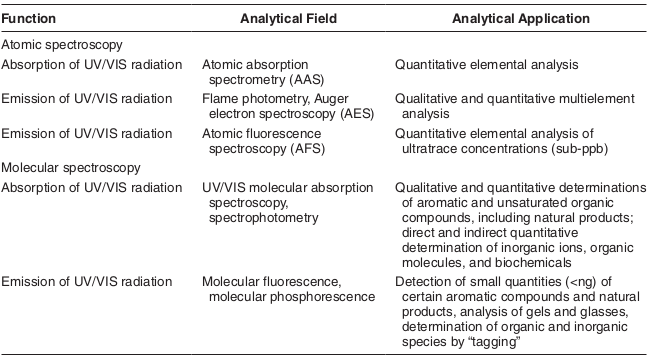
\includegraphics[width=0.9\textwidth]{2021-01-02_17-55.png}
\end{table}
紫外线和可见辐射与物质的相互作用可以定性地鉴定分子和多原子物质,包括离子和
络合物。可以获取有关分子和多原子物种(尤其是有机分子)的结构信息。该定性信息
通常是通过观察UV/VIS光谱,UV吸收和可见辐射随分子的波长而获得的。图\ref{fig:5.1}
(a)至(c)显示了某些有机化合物的典型紫外吸收光谱。光谱可以绘制成波长与吸光度,
透射率或摩尔吸收率$\varepsilon$的关系。随后定义摩尔吸光率。在图\ref{fig:5.1}中
,将溶解在乙醇中的吡啶的吸收光谱绘制为$\log\varepsilon$与波长(以埃为单位)的
关系。图\ref{fig:5.1}(b)和(c)绘制为吸光度与波长(nm)的关系。在这些光谱中看到
的较旧的波长单位为$\mu$m;该单位已被国际系统单位(SI)单位nm取代。注意
图\ref{fig:5.1}(b)和(c)中需要稀释。在图\ref{fig:5.1}(b)中,将溶液以1:10的比例
稀释,使峰在275 nm处成比例。在图\ref{fig:5.1}(c)中,浓度为0.140 g/L时,在230和
222 nm处的吸光度峰不合比例。将该溶液稀释至0.038 g/L的浓度,并在较小光程
的池中运行。

\begin{figure}[htpb]
    \centering
    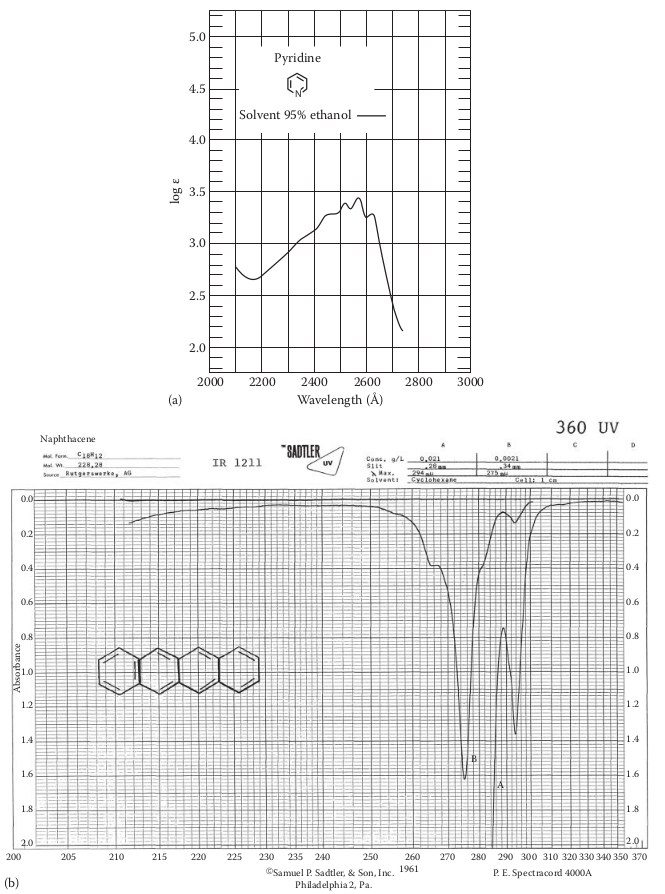
\includegraphics[width=0.95\textwidth]{2021-01-02_19-26.png}
\end{figure}
%\addtocounter{figure}{-1}
\begin{figure}[htpb]
    \centering
    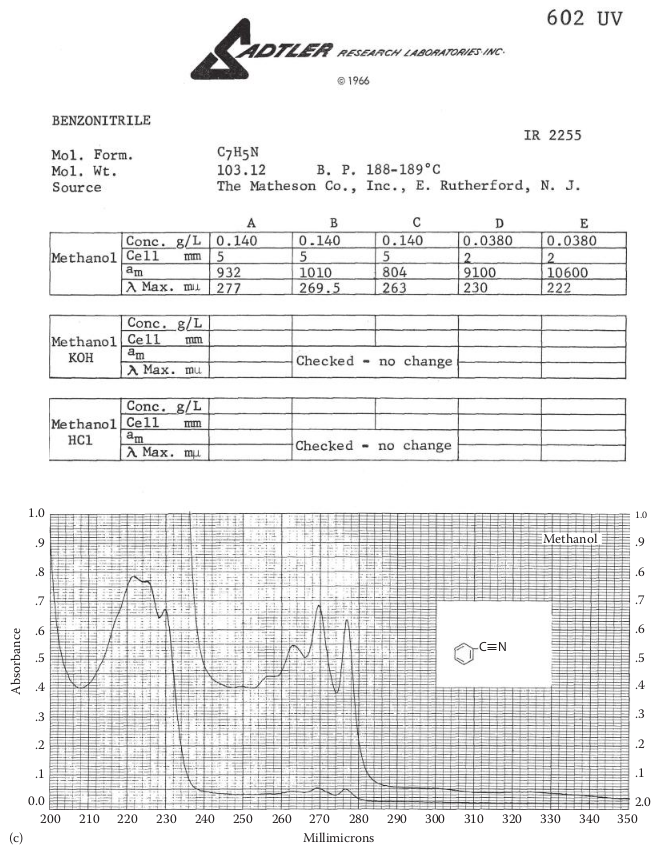
\includegraphics[width=0.95\textwidth]{2021-01-02_19-17.png}
    \caption{几种有机分子溶液的紫外吸收}
    \label{fig:5.1}
\end{figure}

还可以通过研究分子或多原子物质对紫外线和可见辐射的吸收或发射来获得定量信息。
作为一个非常简单的示例,我们可以查看红色溶液(例如红色墨水在水中)的吸收光谱
(图\ref{fig:5.2})。可以看出,对于无色纯净水样品(如虚线所示),所有波长的
白光(包括所有红色波长)都通过样品透射。如果我们向水中添加一滴红色墨水,使溶液
看起来呈浅红色,则光谱表明已吸收了部分蓝色和部分黄色的光,但已透射了所有红色
的光。如果我们在水中添加更多的红色墨水制成深红色溶液,则大部分蓝色和黄色光已被
吸收,但所有红色光都已透射。每种情况下,落在眼睛或检测器上的红光量都相同。溶液
中的墨水量与吸收的蓝光和黄光有关,与透射的颜色无关。我们可以在水中构造一系列
已知量的红色墨水,并通过测量在例如450 nm处吸收的光量来定量测量其他墨水溶液。
样品(尤其是溶液)中物种的浓度通常使用UV/VIS吸收光谱法或荧光光谱法进行测量。
浓度或浓度变化的测量可用于计算化学系统的平衡常数、反应动力学和化学计量。通过
UV/VIS光谱仪进行的定量测量在环境监控、食品和饮料制造等工业过程控制、药品质量
控制和临床化学等方面很重要。分子激发后,分子以多种方式发生辐射。荧光和磷光是
两个过程。
\begin{figure}[htpb]
    \centering
    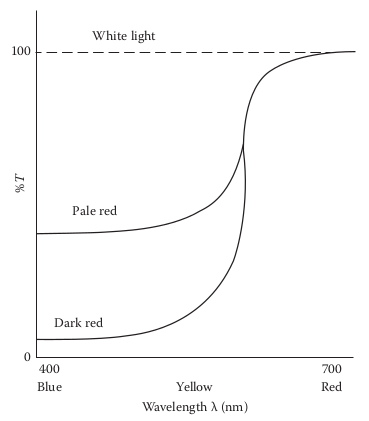
\includegraphics[width=0.6\textwidth]{2021-01-02_19-22.png}
    \caption{可见吸收示例}
    \label{fig:5.2}
\end{figure}
\subsection{分子中的电子激发}
分子由原子组成,这些原子通过共享电子而保持在一起,形成化学键。分子中的电子以
量子理论定义的离散能级在分子轨道中移动。当电子的能量最小时,分子处于最低能量
状态或基态。分子可以吸收辐射并移动到更高能量的状态或激发状态。当分子激发时,
外壳(价)电子移动到能量更高的轨道。将电子移动到更高能态的过程称为电子激发。
为了使辐射引起电子激发,它必须在电磁光谱的可见光或紫外线范围内。分子吸收或发射
的频率与辐射能量之间的关系是$\Delta E = h\nu$。所需的实际能量取决于电子的基态
$E_0$和激发态$E_1$之间的能量差。关系描述为
\begin{equation}
    \Delta E = E_1 - E_0 = h\nu
    \label{5.1}
\end{equation}
$E_1$是激发态能量;$E_0$是基态能量。
可能需要在常规化学教科书或参考书目中列出的Chang或Zumdahl的教科书中查看键合,
分子轨道,路易斯结构和有机化学的主题,以帮助您理解随后讨论的材料。讨论将集中在
有机分子上,因为键合相对容易理解。无机分子也像有机分子与金属离子的络合物一样
吸收和发射紫外线和可见光,但是由于d和f轨道中的电子,无机分子中的键合以及过渡
金属与较重元素的络合物也很复杂。

分子中的价电子跃迁涉及三种不同类型的电子。首先是涉及单键的电子,例如烷烃中碳
和氢之间的电子。这些键称为sigma($\sigma$)键。激发$\sigma$键中的电子所需的
能量通常大于200 nm的UV光子。因此,烷烃和其他饱和化合物(仅具有单键的
化合物)不吸收紫外线辐射,因此通常非常可用作研究其他分子的透明溶剂。这种
不吸收性化合物的一个例子是正己烷(\ce{C6H14})。

接下来,我们使电子参与双键和三键(不饱和键)。这些键包括一个$\pi$键。具有$\pi$
键的化合物的典型例子是烯烃,炔烃,共轭烯烃和芳族化合物(图\ref{fig:5.3})。
$\pi$键中的电子相对容易被激发。这些化合物通常在紫外线或可见光区域吸收。
\begin{figure}[htpb]
    \centering
    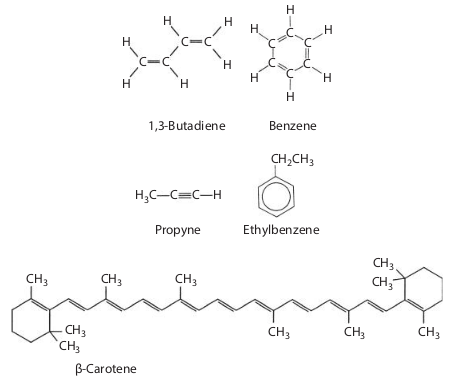
\includegraphics[width=0.75\textwidth]{2021-01-03_01-28.png}
    \caption{含$\pi$键有机物示例}
    \label{fig:5.3}
\end{figure}

原子间不参与原子键合的电子是分子中的第三类电子。对于非键合电子,这些被称为$n$
电子。在饱和烃中,碳和氢的外壳电子都参与键合;因此,这些化合物不具有任何$n$
电子。但是,含有氮,氧,硫或卤素的有机化合物通常含有不键合的电子(图
\ref{fig:5.4})。由于$n$电子通常被UV或可见光辐射激发,因此许多包含$n$电子的
化合物都会吸收UV/VIS辐射。
\begin{figure}[htpb]
    \centering
    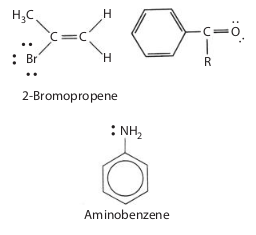
\includegraphics[width=0.5\textwidth]{2021-01-03_01-32.png}
    \caption{含非键有机物示例}
    \label{fig:5.4}
\end{figure}

图\ref{fig:5.5}中显示了在相邻原子上的原子轨道上的两个s电子结合形成$\sigma$键的
示意性能量图。轨道是守恒的;因此,形成两个分子轨道:
一个$\sigma$成键轨道和一个能量更高的$\sigma^\ast$反键轨道。$\sigma$和$\sigma
^\ast$之间的能量差等于$\Delta E$,如大箭头所示。每个原子都有三个2p原子轨道。
这些p轨道中的一个可以与相邻原子上的p轨道重叠,以形成第二组$\sigma$轨道。其他
两个p轨道可能会发生侧向重叠,形成$\pi$成键和$\pi^\ast$反键轨道。形成一组$\pi$
轨道的示意性能量图如图\ref{fig:5.6}所示,大箭头显示了$\pi$成键轨道和$\pi^\ast$
反键轨道之间的能量差。如果p轨道充满一对电子,它将不会形成键。图\ref{fig:5.7}
显示了一个填充的原子p轨道(在右边的原子中)可以形成一个非键合$n$轨道,该能量
不会从原子轨道上转移出来,而每个原子上部分填充的p轨道重叠形成一对
$\pi$键和$\pi^\ast$键轨道。
\begin{figure}[htpb]
    \centering
    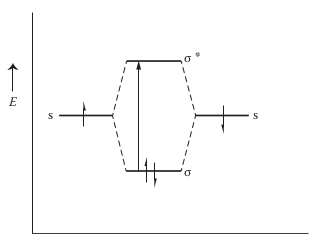
\includegraphics[width=0.5\textwidth]{2021-01-03_01-35.png}
    \caption{两个s原子轨道形成$\sigma$成键和$\sigma^\ast$反键分子轨道}
    \label{fig:5.5}
\end{figure}
\begin{figure}[htpb]
    \centering
    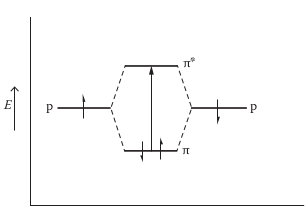
\includegraphics[width=0.5\textwidth]{2021-01-03_01-54.png}
    \caption{两个p原子轨道形成$\pi$成键和$\pi^\ast$反键分子轨道}
    \label{fig:5.6}
\end{figure}
\begin{figure}[htpb]
    \centering
    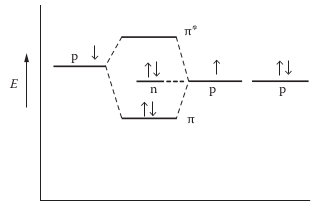
\includegraphics[width=0.5\textwidth]{2021-01-03_01-53.png}
    \caption{p原子轨道形成$\pi$成键、$\pi^\ast$反键和非键$n$分子轨道}
    \label{fig:5.7}
\end{figure}

$\sigma$、$\pi$和$n$电子的相对能图如图\ref{fig:5.8}所示,但该一般顺序有例外。
可以看出,将电子从$\sigma$激发到$\sigma^\ast$轨道所需的能量远大于将电子从
$\pi$激发到$\pi^\ast$轨道,或将$n$电子激发到$\sigma^\ast$或$\pi$所需的能量。
结果,将$\sigma$电子激发到$\sigma^\ast$轨道所需的能量大于在UV区域中可用的能量,
但是通常UV辐射足以将$\pi$轨道中的电子激发到$\pi^\ast$反键轨道,
或将$n$个电子激发到$\pi^\ast$或$\sigma^\ast$。
\begin{figure}[htpb]
    \centering
    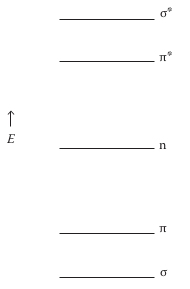
\includegraphics[width=0.25\textwidth]{2021-01-03_01-58.png}
    \caption{$\sigma$成键、$\sigma^\ast$反键、$\pi$成键、$\pi^\ast$反键和非键
    $n$分子轨道能级示意图}
    \label{fig:5.8}
\end{figure}
\subsection{分子吸收}
量子力学为理解分子轨道的相对能级,以及它们如何随结构变化提供理论基础。量子力学
还生成一组“选择规则”,以预测分子中发生的跃迁。分子中发生的跃迁受这些量子力学
选择规则支配。选择规则“允许”某些转换,而“禁止”进行其他转换。选择规则超出本文的
范围,但可以在大多数物理化学文章中或在参考书目中列出的Ingle和Crouch的文章中
找到。与规则一样,也有例外,并且确实发生许多禁止的过渡,并且
可以在UV/VIS光谱中看到。

当分子被电子激发时,电子从占据最高的分子轨道移动到最低的未占据的轨道,该轨道
通常是反键轨道。$\pi$键中的电子被激发成反键$\pi^\ast$轨道,$n$个电子被激发到
$\sigma^\ast$或$\pi^\ast$轨道。

有机分子和无机分子都可能表现出UV/VIS辐射的吸收和发射。吸收可见光或紫外线的
分子基团称为生色团,在希腊语中称为色度(chromophores)。例如,为了发生
$\pi\to\pi^\ast$跃迁,分子必须具有带有不饱和键(例如C$=$C, C$=$O和
C$=$N)的发色团。具有这些类型的生色团的化合物包括烯烃,酰胺,酮,羧酸和肟
等。通常在UV/VIS区域发生的另一种过渡是$n\to\pi^\ast$过渡,因此包含具有未键合
电子的原子的有机分子应能够吸收UV/VIS辐射。这样的原子包括氮,氧,硫和卤素原子,
尤其是Br和I。表\ref{tab:5.2}列出了一些用作生色团的典型有机官能团。表
\ref{tab:5.3}列出了有机化合物的类型及其最大吸收波长,即吸收最多光的波长。一些
化合物具有一个以上的吸收峰,因此列出了多个“最大值”。诸如烷烃之类的化合物仅包含
$\sigma$键,它们不吸收可见光或UV区域的辐射。
\begin{table}[htbp]
    \centering
    \caption{UV/VIS下有吸收的有机官能团}
    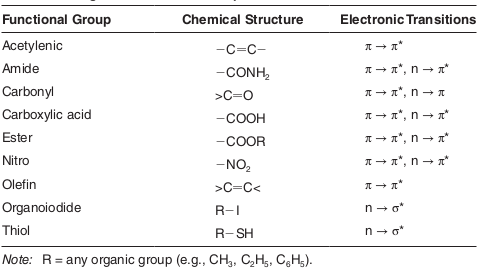
\includegraphics[width=0.7\textwidth]{2021-01-03_09-35.png}
    \label{tab:5.2}
\end{table}
\begin{table}[htbp]
    \centering
    \caption{典型有机官能团最大吸收波长}
    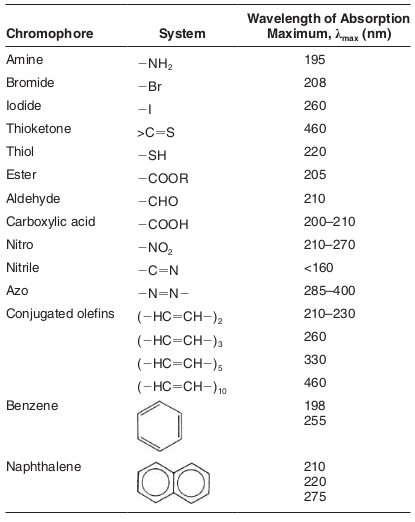
\includegraphics[width=0.6\textwidth]{2021-01-03_09-36.png}
    \label{tab:5.3}
\end{table}

过渡金属化合物通常是有色的,表明它们吸收光谱可见部分的光。这是由于存在未填满的
d轨道。吸收带最大值的确切波长取决于d轨道电子的数量,化合物的几何形状以及与
过渡金属配位的原子。
\subsection{摩尔吸光系数}
上一章我们介绍涉及光程和样品浓度的Beer定律,其中,$\varepsilon$为摩尔吸光系数。
为给定波长、给定浓度下,所吸收的辐射。
\begin{equation}
    A = \varepsilon l c
    \label{5.2}
\end{equation}
浓度$c$的单位是mol$\cdot$L$^{-1}$,光程$l$的单位是cm,那么,$\varepsilon$的单位
为L$\cdot$mol$^{-1}\cdot$cm$^{-1}$。通常,$\varepsilon\approx 10^4 - 10^5$ 
范围的跃迁是允许的,10--100范围内的跃迁,是禁阻的。较高的$\varepsilon$值,对
特定波长的光,有强吸收;较低值,对应弱吸收。$\varepsilon$表明特定波长下,分子
的物理性质。最大吸收波长的符号为$\lambda_{max}$,同理,最大的摩尔吸光系数表示
为$\varepsilon_{max}$。表\ref{tab:5.4}列出一些常见有机分子$\lambda_{max}$和
$\varepsilon_{max}$的典型值。
\begin{table}[htbp]
    \centering
    \caption{常见发色团典型的最大吸收峰和摩尔吸光系数}
    \includegraphics[width=0.6\textwidth]{2021-01-04_20-57.png}
    \label{tab:5.4}
\end{table}

测量吸收的波长范围比吸收带宽要窄,所以摩尔吸光系数不能直接衡量电子跃迁的可能性
。摩尔吸光系数,在整个波段范围内的不同波长处,是不相同的。有几个与跃迁概率
直接相关的基本量,如爱因斯坦系数和振荡器强度$f$。
\subsection{紫外吸收曲线形状}
图\ref{fig:5.1}是溶液中有机分子典型的紫外吸收光谱。每个光谱看起来非常简单,
在很宽的波长范围内,具有较宽的吸收“带”,而不是在红外(IR)光谱中看到的众多的
较窄的吸收峰。分子中每个电子的能级都有与其相关的多个振动和转动能级,导致吸收带
非常宽。电子从基态到激发态的跃迁,所达到的不止一个激发态的振动和转动能级。
电子跃迁振动和转动能级示意图如图\ref{fig:5.9}所示。在基态,仅显示最低的振动
能级,带有四个转动子能级。室温下,多数分子处于最低振动状态的基态。激发态中,
显示四个振动子能级,每个振动能级里,有差别很小的转动子能级。在许多可能的跃迁
类型中,选取四种显示在图中;每一个箭头对应一个吸收波长。电子跃迁是有大量波长
组成连续的吸收带。尽管每一个跃迁是量子化的,靠近振动能级,或者,靠近转动能级的
能量空间,导致电子跃迁是一个带光谱。如图\ref{fig:5.10}所示。
\begin{figure}[htpb]
    \centering
    \includegraphics[width=0.55\textwidth]{2021-01-08_20-45.png}
    \caption{电子跃迁能量带源于电子具有多个振动和转动能级}
    \label{fig:5.9}
\end{figure}
\begin{figure}[htpb]
    \centering
    \includegraphics[width=0.85\textwidth]{2021-01-08_20-48.png}
    \caption{UV吸收带}
    \label{fig:5.10}
\end{figure}

吸收带的特征在于其形状,即其宽度和强度。带的形状主要由振动能级间隔和每个振动
跃迁的强度决定。强度分布与跃迁到给定振动能级的可能性有关。跃迁概率可以使用
弗兰克-康登(Franck-Condon)原理确定。 参见Hollas和Lambert等人的文章。可以说,
如果我们有一百万个分子,即使它们在激发前大多处于基态振动状态,但在激发后它们
可能处于各种振动状态。引起电子激发到每个振动能级所需的辐射能略有不同,并且会
通过转动能的变化进一步改变。因此,当紫外辐射落在这一百万个分子上时,它会在许多
波长处被吸收。吸收波长的总范围可能会延长至100 nm范围内。分子转动能级,使得吸收
线更加变成单一的吸收带。吸收线数目的增加,使得线彼此接近,但不会增加吸收带的
总宽度。这是因为引入的转动能级与振动能级相比,很小,与电子跃迁相比,就更小了。
因此,紫外辐射是吸收带,而不是离散的波长。

在许多实际测试中,UV/VIS光谱显示了不同的振动能级。例如,气相中简单的分子的振动
跃迁,经常与电子跃迁叠加在一起,如图\ref{fig:5.11}所示气相苯的吸收光谱。宽
谱带顶部的尖峰,是振动能级的“精细结构”。溶液中的分子(如图\ref{fig:5.1})通常
不具备这种振动结构,是由于溶剂和溶质分子间的相互作用导致的。相比于气相苯的吸收
,溶液中苯的吸收光谱(如图\ref{fig:5.12}),大多数的精细结构消失不见。可见,
精细结构源于转动能级,在常规的UV/VIS中,无法观察到;商业仪器没有这么高的解析度
,可以观察到这些线。
\begin{figure}[htpb]
    \centering
    \includegraphics[width=0.85\textwidth]{2021-01-08_22-16.png}
    \caption{气相苯的吸收光谱}
    \label{fig:5.11}
\end{figure}
\begin{figure}[htpb]
    \centering
    \includegraphics[width=0.55\textwidth]{2021-01-08_22-18.png}
    \caption{溶液中苯的吸收光谱}
    \label{fig:5.12}
\end{figure}
\subsection{UV/VIS光谱的溶剂}
绝大多数的吸收光谱是在溶液中测量的。溶质必须可溶于溶剂,并且溶剂必须在目标
波长范围内是透明的(无吸收)。形成溶液的使能量降低。溶质和溶剂之间的分子间
吸引力必须大于溶质-溶质和溶剂-溶剂之间的吸引力。溶液形成所涉及的力是偶极-偶极
吸引,氢键和范德华力。极性起着主要作用,并产生了“like dissolves like”的规则。
与非极性溶剂相比,极性物质在极性溶剂中的溶解更容易。溶质要完全溶解是很重要的。
未溶解的粒子会散射来自光源的光。这可能会导致定性和定量分析中的严重误差。

溶剂有时会严重影响光谱的形状。极性溶剂通常会消除光谱中的振动精细结构。溶剂也会
移动吸收带的位置。对于光谱的可见区域,可以使用样品可溶于其中的任何无色溶剂。

UV/VIS光谱学中使用的常见溶剂及其低波长截止值列于表\ref{tab:5.5}中。在比截止
波长短的波长处,溶剂吸收太强而无法在标准的1 cm样品池中使用。临界值受溶剂纯度
的影响。对于光谱学,溶剂应属于光谱或光谱化学级,符合美国化学学会规定的纯度要求。
\begin{table}[htbp]
    \centering
    \caption{常用紫外光谱测试的溶剂及其截止波长}
    \label{tab:5.5}
    \includegraphics[width=0.5\textwidth]{2021-01-08_22-37.png}
\end{table}
\section{仪器}
\subsection{光学系统}
光谱仪是测量吸收或透过的光的强度,并作为波长的函数的仪器设备。单光束或双光束
用于分子吸收光谱的测量。单光束系统和它的三个缺点,已经在上一章讨论过。绝大多数
商业仪器都使用双光束系统,我们重点讨论一下。

双光束系统将辐射源分成强度相等的两份光路。两束光穿过两条长度相同的光路;
\emph{参比}池放在一个路径中,而\emph{样品}池则在另一路径中。然后比较穿过两池的
两个光束的强度。由于功率波动,光学系统损失的辐射(例如,样品池表面和反射镜,
溶剂吸收的辐射等),导致辐射强度变化对于两个光束都应相等,以校正这些误差源。
用于吸收光谱的色散光谱仪被称为分光光度计,该色散光谱仪具有一个或多个出口狭缝和
光电检测器,该光电检测器将两个光束的强度与波长成比例。

商用UV/VIS光谱仪设计为在200--800 nm范围内的空气中与空气一起运行。用干燥的氮气
吹扫光谱仪可以观察到低至175 nm的波长。如前所述,对于较低的波长,必须将光谱仪
置于真空下或用不吸收气体吹扫。在分析上,由于需要真空的仪器固有的困难和费用,
真空紫外线区域对常规分析的重要性不高。

使用滤光片进行波长选择和光电检测器的简单光学系统称为光度计。光度计用于可见光
区域和紫外线区域。例如,紫外光度计通常用作高效液相色谱(HPLC)中的检测器,但已
被光电二极管阵列(PDA)取代。 HPLC检测器将在后续章节中详细讨论。

所有用于吸收测量的光谱仪都需要一个光源,一个波长选择设备,一个样品架和一个
检测器。可以从许多商业仪器公司获得完整的UV/VIS和UV/VIS/近红外(NIR)系统,包括
安捷伦科技公司,PerkinElmer,Shimadzu Scientific Instruments和Thermo Fisher 
Scientific。这些大型公司各自提供具有不同功能的5至8个版本的系统。他们的网站提供
应用程序,有关使用仪器的视频,教程以及许多其他有用的信息。
\subsection{辐射源}
用于分子吸收测量的辐射源必须产生连续波长的光。理想地,光源的强度在所有发射的
波长上将是恒定的。传统上,用于UV/VIS光谱的两个最常见的辐射源是钨灯和氘灯。钨灯
的功能类似于普通的白炽灯泡。它包含一个钨丝,该钨丝被电加热至白热并产生连续
光谱。它有两个缺点:短波长($<$ 350 nm)的辐射强度低;此外,为了保持恒定的强度,
必须小心地控制灯电流。但是,这些灯通常是稳定,坚固且易于使用的。发射强度随波长
变化,如图\ref{fig:5.13}所示。这些曲线的形状是加热到白炽灯的固体连续输出的典型
特征。产生这种曲线的白炽体称为黑体辐射器。连续发射是由于固体(在这种情况下是
钨丝)中的热激发跃迁引起的。黑体辐射器的强度与波长的关系图取决于发射材料的温度
,而不取决于其化学成分。钨灯在可见光范围内最有用,通常在分光光度法中使用,随后
进行讨论。由于仅在可见光区域使用灯泡,因此灯泡可以由玻璃而不是石英制成。紫外光
的传输需要石英。与现代汽车前照灯中的灯类似,钨卤素灯已取代了现代仪器中较旧的
钨灯。钨卤素灯有一个石英灯泡,主要用来承受灯的高工作温度。该灯比钨灯高效得多,
并且使用寿命更长。钨卤素灯的波长/强度输出如图\ref{fig:5.14}所示。
\begin{figure}[htpb]
    \centering
    \includegraphics[width=0.75\textwidth]{2021-01-09_10-11.png}
    \caption{黑体辐射的发射强度}
    \label{fig:5.13}
\end{figure}
\begin{figure}[htpb]
    \centering
    \includegraphics[width=0.85\textwidth]{2021-01-09_10-13.png}
    \caption{(a)商用钨卤灯发射光谱;(b)商用氘弧灯发射光谱}
    \label{fig:5.14}
\end{figure}

\emph{氘弧灯}由石英灯泡中的氘气(\ce{D2})组成,放电时通过氘气。分子被电激发,
被激发的氘分子解离,发出紫外线。氘分子解离成原子会导致在从0到分子激发能的连续
能量范围内发出UV光子。这会导致灯在160--400 nm的范围内发出连续的(宽带)UV光谱,
而不是窄线原子发射光谱。该灯稳定,坚固并且被广泛使用。使用氘代替氢气的效果是,
在UV范围的短波长端发射强度增加多达三倍。虽然氘比氢更昂贵,但获得所需的高强度
的光源。图\ref{fig:5.14}(b)给出了氘弧灯的发射光谱。

\emph{氙弧灯}的工作方式类似于氘灯。氙气通过电流会在200--1000 nm范围内产生强烈
的辐射。它们提供非常高的辐射强度,并且它们不需要预热时间,因此被广泛用于现代
UV/VIS仪器中。该灯用于荧光光谱法,其灯的原理图和光谱见后续章节。如今,许多
UV/VIS光谱仪都使用氙气闪光灯,氙气闪光灯仅在读取读数时才会闪烁。它们不需要预热
时间,并且只需很少的电能。用这种类型的灯可以消除光降解,因为样品不会暴露在大量
的辐射或热量下。

最近引入的重要光源是发光二极管(LED)。 LED由掺有杂质的半导体材料芯片组成,以
形成PN结(见图\ref{fig:5.21})。电流从阳极的p侧流向阴极的n侧。电荷载流子,电子
和空穴从具有不同电压的电极流入结中。当电子遇到空穴时,它会降到较低的能级并发射
光子。发出的光的波长(其颜色)取决于形成PN结的材料的带隙能量(图
\ref{fig:5.15}(a)和\ref{fig:5.20})。 LED原理图如图\ref{fig:5.15}(b)所示。
\begin{figure}[htpb]
    \centering
    \includegraphics[width=0.75\textwidth]{2021-01-09_11-55.png}
    \caption{(a)LED中电子和空穴;(b)LED构造}
    \label{fig:5.15}
\end{figure}

现在,可以使用各种可见颜色的商用LED以及发射IR和UV的LED。发出紫外线的LED通常由
氮化硼(\ce{BN}),氮化铝(\ce{AlN}),氮化铝镓(\ce{AlGaN})和氮化铝镓铟
(\ce{AlGaInN})制成。为了创建用于可见光谱的白光源,使用了两种方法。一种是将
红色,绿色和蓝色LED混合使用以产生白光。红色LED是第一个实际应用的LED,也是第
一个商业化的LED,它由磷化镓(\ce{GaP}),砷化镓磷化物(\ce{GaAsP}),砷化铝镓
(\ce{AlGaAs})和磷化铝镓铟磷(\ce{AlGaInP})制成。绿色LED基于氮化铟镓
(\ce{InGaN}),磷化铝镓(\ce{AlGaP})和类似材料。蓝色LED由氮化铟镓
(\ce{InGaN}),硒化锌(\ce{ZnSe})和其他材料制成。第二种方法是在开发高强度
蓝色LED之后实用的,它是使用蓝色LED和基于氧化钇铝(也称为YAG)等材料的荧光粉
涂层。磷光体产生的黄光与蓝光结合时会变成白色,这与标准荧光灯泡的工作方式
非常相似。
\subsection{单色器}
单色器的目的是根据波长分散辐射,并允许选定的波长照亮样品。衍射光栅用于在现代
仪器中散射光,如前所述。现代系统中的单色器,例如安捷伦科技公司的Cary分光光度计
,可以以高达2000--3000 nm/min的速率扫描,并具有摆率(在不进行测量的情况下,
在波长之间移动的时间)高达16000 nm/min,以适应制药和生物技术实验室所需的
高通量测量。

新的衍射光栅技术允许进行几年前无法进行的测量。由离子束或激光束光刻技术产生
的前一章中讨论的衍射光栅,由于表面粗糙度,会产生杂散光(不需要的波长的光)。
如今,为优化与全息技术一起使用的蚀刻工艺而开发的新型专有制造方法可大大改善
衍射光栅,例如Shimadzu Scientific Instruments(www.ssi.shimadzu.com)的
“Lo-Ray-Ligh”光栅。Lo-Ray-Ligh光栅具有低至0.00005 \%的超低杂散光值,可在高达
8.5吸光度单位的情况下以完全线性的方式进行吸光度测量。图\ref{fig:5.16}(a)比较了
使用Lo-Ray-Ligh光栅在UV-2700上获得的吸收光谱与在常规光谱仪上获得的吸收光谱。
图\ref{fig:5.16}(b)展示了超过8.5个吸光度单位的线性。这样可以测量高吸收性材料,
例如太阳镜偏光镜和焊接面罩。在下一节中将给出一些示例。
\begin{figure}[htpb]
    \centering
    \includegraphics[width=0.85\textwidth]{2021-01-09_12-14.png}
    \caption{(a)左:使用Lo-Ray-Ligh光栅的UV-2700光谱仪获得的光谱;右:常规光谱
    仪获得的光谱(超出范围)(b)UV-2700校正曲线,吸光度为8.5依然保持线性}
    \label{fig:5.16}
\end{figure}
\subsection{检测器}
最早用于可见光谱的检测器是人眼。仍然有专为视觉观察颜色和强度而设计的分光镜和
颜色比较器。

大多数现代仪器都依赖于{\bf 光电转换器},将光子转换成电信号的检测设备。光电转换
器的表面可以吸收辐射能。吸收的能量要么导致电子发射,从而产生光电流,要么将电子
移动到固体半导体的导带中,从而导致电导率增加。这些检测器有几种常见形式,包括
势垒层电池、光电倍增管(PMT)和半导体检测器。
\subsubsection{势垒层电池}
在势垒层电池(也称为光伏电池)中,吸收辐射后会在金属和半导体的界面处产生电流。
例如,将银涂在半导体(例如硒)上(参见图\ref{fig:5.17}),该半导体与诸如铁之类
的坚固金属基体相连。为了制造这些电池,将硒放入容器中,并将气压降低至真空。银被
电加热,其表面熔化和汽化。银蒸气覆盖硒表面,形成非常薄但均匀分布的银原子层。
落在表面上的任何辐射都会在硒-银界面处产生电子和空穴。硒和铁之间似乎存在一个
屏障,可以阻止电子流入铁中。电子流向银层,空穴流向铁。电子被银收集。这些收集的
电子通过外部电路向空穴迁移。以这种方式产生的光电流与撞击的光子数量成正比。
\begin{figure}[htpb]
    \centering
    \includegraphics[width=0.65\textwidth]{2021-01-09_12-34.png}
    \caption{势垒层电池}
    \label{fig:5.17}
\end{figure}

势垒层电池在照相机和低成本便携式仪器中用作检测器。响应范围是350--750 nm。这些
检测器有两个主要缺点:它们在弱光下不灵敏并且显示出\emph{疲劳感},也就是说,
在持续暴露
于光线下电流会逐渐下降。从好的方面来说,它们不需要外部电源,并且非常坚固。
\subsubsection{光电倍增管}
PMT是一种非常常见的检测器。 PMT是密封的,抽空的透明外壳(石英或玻璃),包含
光电发射阴极、阳极和几个称为倍增极的其他电极。光电发射阴极是涂有碱金属或元素
混合物(例如Na/K/Cs/Sb或Ga/As)的金属,当被光子撞击时会发射电子。 PMT是真空
光电管的更复杂的版本,图\ref{fig:5.18}(a),其中仅包含光电发射阴极和阳极。
光电流仅限于从阴极发射的电子。在PMT中,图\ref{fig:5.18}(b)中,额外的倍增极将
可用电子“相乘”。喷射的电子被吸引到倍增极,该倍增极相对于阴极保持在正电压。到达
倍增极后,每个电子都会撞击倍增极的表面,并使表面再发射出几个电子。这些发射的
电子又被第二倍增极所吸引,在第二倍增极中,类似的电子发射和更多的倍增发生。重复
该过程数次,直到大量电子到达阳极(即集电极)为止。落在收集器上的电子数量是落在
检测器上的光强度的量度。在此过程中,单个光子可能会产生许多电子并发出高信号。
因此,倍增极工作在提供稳定信号的最佳电压下。商业PMT可能有九个或更多倍增极。
每个光子的增益可能高达$10^9$个电子。探测器系统的噪声水平最终会限制增益。例如,
增加倍增极之间的电压会增加信号,但是如果电压太高,来自检测器的信号就会变得
不稳定或嘈杂。在实践中,较低的增益和较低的噪声水平可能是更可取的。
\begin{figure}[htpb]
    \centering
    \includegraphics[width=0.75\textwidth]{2021-01-09_12-39.png}
    \caption{(a)真空光电管;(b)PMT构造图(俯视)}
    \label{fig:5.18}
\end{figure}

PMT对紫外线和可见辐射极为敏感。实际上,它们是如此敏感,以至于必须注意不要将
PMT暴露在强光下,以免造成损坏。有各种各样的光发射表面可用,它们可以响应不同的
波长范围。检测器信号与波长的关系曲线称为响应曲线。图\ref{fig:5.19}显示了商用
PMT的一些响应曲线。选择PMT检测器,以使其对目标波长范围具有最大响应。例如,IP28
在800 nm处不可用,但R136和Ga/As PMT检测器在此范围内有响应。PMT的响应时间非常快
,但是它们的暗电流限制了它们的灵敏度。暗电流是没有辐射落在检测器时,检测器发出
的恒定小信号。可以通过冷却检测器外壳来最小化或消除暗电流。为此目的,商业上
可加入冷却装置。
\begin{figure}[htpb]
    \centering
    \includegraphics[width=0.65\textwidth]{2021-01-09_12-40.png}
    \caption{商用PMT响应曲线}
    \label{fig:5.19}
\end{figure}
\subsubsection{半导体检测器:二极管和二极管阵列}
固态半导体材料在电子设备和仪器中非常重要,包括用作辐射探测器。为了理解半导体
的行为,有必要简要描述这些材料中的键合。

当大量原子键合形成固体(例如固体硅)时,单个原子中存在的离散能级会扩散到固体中
的能带中。价电子不再局限于空间中的给定原子。能带的宽度随着固体中原子间间距的
减小而增加。至少部分被电子占据的最高能带称为价带;价带正上方的能带称为导带。
价带和导带被一个禁能范围隔开(量子力学禁止)。这种分离的幅度称为带隙,如图
\ref{fig:5.20}示意性地显示了一组能带和带隙。如果固体的价带在0 K的温度下完全
充满,则该材料是{\bf 半导体}或{\bf 绝缘体}。半导体和绝缘体之间的差异由带隙的
大小定义。如果$E_g \leq 2.5 \text{ eV}$,则该材料为半导体;如果$E_g >2.5$ eV,
则该材料为绝缘体。第三类材料,导体,在0 K处具有部分填充的价带。
\begin{figure}[htpb]
    \centering
    \includegraphics[width=0.65\textwidth]{2021-01-09_17-49.png}
    \caption{固体材料价带,$E_g$为带隙}
    \label{fig:5.20}
\end{figure}

半导体器件中最常使用的两个元素是硅和锗。两者均以固态共价键合且均属于元素周期表
的第IVA族。(在新的国际纯粹与应用化学联合会(IUPAC)术语中,该组也称为第14族,
在某些文本中,该组也称为IVA。)其他半导体包括\ce{GaAs},\ce{CdTe},\ce{InP}
以及其他无机和有机化合物。大多数半导体是共价键结合的固体。CRC的化学和物理手册中
列出了半导体的带隙能。

硅具有价电子结构\ce{3s^2{}3p^2}。部分填充的p轨道可能会导致人们假设硅具有部分填充
的价带,因此将成为导电体。因为硅是共价键合的,所以两个3s电子和两个3p电子占据了
\ce{sp^3}杂化轨道。这产生具有两个电子能带的固体,每个能带具有四个紧密间隔的子
能级,每个电子能带位于\ce{Si}的价电子壳中。四个电子占据并填充了0 K的价带,
因此不导电。但是,在高于0 K的温度下,一些电子会从价带热传导到导带;在那里,
它们成为电的导体。当电子离开价带时,它会留在也可以移动的正空穴之后,从而产生
一个电子-空穴对。电子和空穴都是半导体中的电荷载流子。诸如\ce{Si}和\ce{Ge}之类
的半导体称为本征半导体。它们的行为是纯材料的带隙和能带结构的结果。

可以通过向这些元素之一掺杂VA族元素(如砷或锑)或IIIA族元素(如铟或镓)来提高
电导率。掺杂是指向基质材料中添加其他物质。添加的物质称为掺杂剂。与掺杂原子关联
的电子与主体的能级不同,并且可能处在主体禁止的能级上。由添加掺杂剂引起的电导率
称为外在导电。VA族元素具有额外的电子(或额外的负电荷)。该电子不像主体的共价
键合电子那样牢固地保持,并且需要更少的能量才能将其移动到导带中。这是n型半导体。
类似地,添加IIIA组元素会导致电子“丢失”;这可以认为是产生了额外的正空穴。来自
掺杂剂原子的这些正空穴可以接受来自价带的电子。将电子移动到受体孔中所需的能量
小于将电子移动到导带中所需的能量。这是p型半导体。在n型半导体中,电子是可移动的
,而在p型半导体中,空穴是可移动的。在本征半导体中,每个激发事件都会形成两个电荷
载流子。在n型或p型非本征半导体中,每个激发事件仅形成一个电荷载流子。

半导体可用作电磁辐射检测器。$ E> E_g$的光子足以在半导体中创建其他电荷载流子。
额外的电荷载体会增加半导体的导电性。通过测量电导率,可以计算出光的强度。选择
具有合适带隙的材料可以在光谱的UV,可见光和IR区域产生光检测器。
\subsubsection{二极管}
二极管或整流器是一种电子设备,仅允许电流在一个方向上流动。如果我们将一个p型
半导体和一个n型半导体放在一起,那么这两种类型之间的结就是一个p–n结,如图
\ref{fig:5.21}所示。它由单片半导体通过将一侧掺杂为p型而另一侧掺杂为n型半导体
而形成。在两种类型相遇的地方形成连接点。在向器件施加任何电势之前,空穴将成为
p侧的主要电荷载流子,而电子将成为n侧的主要电荷载流子。如果我们在p型侧施加
正电势,而在n型侧施加负电势,如图\ref{fig:5.22}所示,则正电荷(空穴)从p区域
流向结,而负电荷从n型区域流向结。在结处或附近,空穴和电子复合并被猝灭。这称为
正向偏置,在这种情况下,电流容易流过半导体。电子-空穴对猝灭产生能量。如果这种
能量以光的形式出现,那么我们有前面讨论过的LED。
\begin{figure}[htpb]
    \centering
    \includegraphics[width=0.55\textwidth]{2021-01-09_18-16.png}
    \caption{没有电势的p-n结}
    \label{fig:5.21}
\end{figure}
\begin{figure}[htpb]
    \centering
    \includegraphics[width=0.55\textwidth]{2021-01-09_18-18.png}
    \caption{向前偏置的p-n结,电池的正极连接p端}
    \label{fig:5.22}
\end{figure}

但是,如果施加的电压方向相反,则载流子的方向相反,如图\ref{fig:5.23}(a)所示。
这些是反向偏置的条件。结区耗尽了移动电荷载流子,不会发生重组,也不会发生明显的
电流流动。由于固有的导电性,总会有少量电流流动。简而言之,p-n结起整流器的作用,
仅在正向偏置下才允许大量电流通过。
\begin{figure}[htpb]
    \centering
    \includegraphics[width=0.55\textwidth]{2021-01-09_18-22.png}
    \caption{(a)反向偏置的p-n结,电池的正极连接n端;(b)光照射在耗尽区,光电
    二极管图例。}
    \label{fig:5.23}
\end{figure}

如果将二极管保持在反向偏压下,并且能量大于带隙能量的光子落在二极管结上(如图
\ref{fig:5.23}(b)所示),则会在耗尽区形成电子-空穴对。这些载流子将流过二极管,
产生的电流与落在二极管上的光的强度成比例。这些检测器涵盖从紫外线(约190 nm)到
近红外(约1000 nm)的光谱范围,但不如PMT灵敏。与PMT相比,它们的动态范围有限,
并且当它们偏离线性时,它们会急剧地变化。
\subsubsection{二极管阵列}
在UV/VIS光谱学中,可以通过扫描整个波长范围并用PMT记录光谱(一次是一个波长)来
获得完整的吸收光谱。尽管现代仪器比旧仪器要快得多,但是使用传统的扫描单色仪系统
需要花费时间。在与另一波长不同的时间测量一个波长的吸收。

在两种情况下,扫描光学系统不能很好地工作。首先是发生快速的化学反应,而常规扫描
太慢而无法追踪反应。第二个是样品仅在有限的时间内可用,而无法进行完整扫描。后者
的实例包括来自液相色谱分离的洗脱液,流动注射系统中的流动物流或化学或制药生产
厂中的工艺物流。在这种情况下,需要同时监视许多波长。理想情况下,应在同一时刻
测量整个光谱范围内的强度。如今,第三个条件常常推动了对快速分析的需求(在许多
行业中都要求高样品通量)通常是24/7全天候无人值守的仪器操作,这缩短了分析
“周转”时间并影响了成本。

线性PDA(LPDA)是开发用于能够同时测量许多波长的光强度的传感器。二极管阵列由嵌入
在一维线性阵列中的单晶中的许多半导体组成。常见的步骤是使用掺杂硅的单晶,它是
n型半导体。少量的IIIA族元素(例如砷)以规则的间隔嵌入到表面中。这产生了局部
p型半导体。半导体装置理想地具有如图\ref{fig:5.24}所示的横截面。该表面包含p–n结
的线性系列或阵列,每个结都是光电二极管。各个二极管称为元件,通道或像素。
\begin{figure}[htpb]
    \centering
    \includegraphics[width=0.85\textwidth]{2021-01-09_19-10.png}
    \caption{PDA}
    \label{fig:5.24}
\end{figure}

PDA布置为电路的一部分。通过给电路中的电容器充电,会在p-n结两端产生反向偏置。
辐射落在阵列上会在p和n区域产生电荷载流子。然后,电子将流向最近的p型半导体,并且
空穴被收集在p型区域中。电流使电容器部分放电。在测量周期结束时,电容器被充电;
充电电流产生的电压与光强度直接相关。在特定元件中形成的电荷载流子的数量取决于
该特定元件紧邻的阵列上的光强度。通过测量每个单独元素上的电荷,可以瞬时测量
光强度与整个光谱范围的波长的关系,但要测量离散的元素。这等于数字紫外线
吸收光谱。

商用多通道仪器的光学布局如图\ref{fig:5.25}所示。在此系统中,来自光源(可能是
氘灯或其他UV/VIS光源)的辐射穿过样品到达全息光栅,在全息光栅中,辐射被波长分开
并导向二极管阵列检测器。不使用出口狭缝。整个光谱区域的测量时间远远少于1 s。
实际上,光谱通常被采集超过1 s并由计算机存储。这种做法提高了测量的信噪比。通过
获取多个测量值,可以累积信号并显着提高灵敏度。
\begin{figure}[htpb]
    \centering
    \includegraphics[width=0.85\textwidth]{2021-01-09_19-13.png}
    \caption{二极管阵列光谱仪光学系统}
    \label{fig:5.25}
\end{figure}

PDA可以覆盖190至1100 nm之间的波长范围。整个波长范围的同时使用提供了多路传输的
优势,并提高了系统的分辨率。系统的分辨率受所涉及的二极管元件数量的限制。典型的
二极管间距为0.025 mm。可以认为每个覆盖了有限的光谱范围。已经开发出了阵列中多达
4096个元素的检测器,尽管1024可能是最常见的数字。

二极管阵列系统最重要的应用是分子光谱,因为通常它们没有原子光谱所必需的分辨率。
在分子光谱学中,最有用的应用领域是(1)扫描快速反应以确定动力学;(2)涉及低光照
水平的应用,得益于光谱可以存储并相互添加,从而增加强度;(3)用于HPLC和毛细管
电泳(CE)的检测器。
\subsection{样品池}
用于UV/VIS光谱的样品可以是固体、液体或气体。针对这些样品类型设计不同类型的
样品池。如下一节所述,专为纳升样品量设计的新型光谱仪样品池。
\subsubsection{液相和气相池}
紫外线吸收或发射光谱学中使用的样品池或比色皿,必须对紫外线辐射透明。最常用的
材料是石英和熔融石英。石英和熔融石英对大多数溶剂也具有化学惰性,它们是坚固且
使用可靠。(注意:这些样品池中绝对不能使用含有氢氟酸或强碱的溶液,例如浓
\ce{NaOH}。此类溶液会腐蚀样品池表面,使其无法用于定量工作。)石英和熔融石英
样品池也是在可见光和NIR区域是透明的,因此这些可以用于UV和可见光区域的所有工作。
这些也是最昂贵的,因此,如果仅使用光谱的可见部分,则可以使用便宜的样品池,
例如Pyrex。

图\ref{fig:5.26}显示了一些典型的、多种尺寸的样品池类型。分光光度法的标准尺寸
一直是1 cm光程长的矩形样品池,该样品池可容纳约3.5 mL溶液,如图\ref{fig:5.26}
左上方所示。有体积小至40 $\mu$L的微体积池(图\ref{fig:5.26}左上角的第二个),
用于工艺流或大量样品常规分析的流通池,用于色谱系统的微流通池以及更大的气体和
高度稀释溶液的路径长度/容积池。图\ref{fig:5.26}底部中间显示了两个流通池。
通常,气室是长路径的气室,例如图\ref{fig:5.26}右上方所示的气室,一旦填充了气体
样本,气室必须能够关闭。样品池技术的创新包括纳米体积(即亚微升体积)的开发,
例如Starna可拆卸微体积(DMV)生物池,一种用于大多数UV/VIS光谱仪的超低体积池。
DMV-Bio的光程长度为0.5、0.2和0.125 mm,标称样品体积分别为2.5、1.0和0.6 $\mu$L。
另一个纳米体积的样品池是来自Hellma Analytics(www.hell-mausa.com)的TrayCell,
其路径长度为0.2或1.0 mm,可以测量和回收低至0.5 $\mu$L的体积(图\ref{fig:5.31}
)。
\begin{figure}[htpb]
    \centering
    \includegraphics[width=0.75\textwidth]{2021-01-09_22-21.png}
    \caption{使用较广的液体样品池}
    \label{fig:5.26}
\end{figure}

为了在可见光谱范围内进行分光光度分析,可以使用玻璃或一次性塑料盒。它们比石英
或熔融石英便宜,但不能在短紫外线波长下使用。聚苯乙烯通常用于可见范围的比色皿
(340--800 nm),而丙烯酸聚合物比色皿可用于285 nm以下。塑料样品池不能与可溶于
塑料的任何有机溶剂一起使用。一次性塑料盒不适用于准确的定量工作。材料之间的价格
差异很大。例如,用于紫外线的高质量1 cm石英样品池的价格约为80美元,而透射范围为
220--3800 nm的1 cm Infrasil®石英样品池(来自Starna,Inc.)的价格约为130美元。
在可见区域使用的相同尺寸的玻璃样品池的价格约为35美元,而1 cm长的塑料一次性
样品池的价格约为10至20美分。微型样品池,流通池和其他专用细胞非常昂贵,每个
样品池的成本为200--500美元。一些光谱仪被设计为使用普通的玻璃试管作为“池”。
这些试管“池”不应用于准确的定量工作。图\ref{fig:5.27}显示了一些典型样品池材料
的透明度。
\begin{figure}[htpb]
    \centering
    \includegraphics[width=0.75\textwidth]{2021-01-09_22-33.png}
    \caption{UV/VIS光谱样品池材质的透过率}
    \label{fig:5.27}
\end{figure}

重要的是正确处理样品池,以获得最佳结果并延长其寿命。为此,分析人员应(1)始终
选择正确的分析样品池;(2)保持样品池清洁并检查是否有污渍,蚀刻痕迹或划痕,这些
改变了电池的透明度;(3)将样品池应保持在不透明的表面上(如果提供);(4)使用前
彻底清洁,并在填充和测量之前用少量样品溶液润洗;(5)请勿将强碱性溶液或氢氟酸
(\ce{HF})溶液放入玻璃,石英或熔融石英电池中;(6)将一次性塑料样品池放入光谱仪
之前,检查其与溶剂的相容性;(7)对于非一次性电池,请务必小心干燥并返回其适当的
存储箱中;(8)切勿用纸制品,制造商推荐的镜头清洁纸或抹布擦拭光学表面。长期不
使用时,应保持样品池清洁干燥存放,以免刮伤光学表面。
\subsubsection{Matched Cells}
使用双光束仪器时,需要两个单元:一个用于参比,一个用于样品。这些样品池的吸收
略有差异是正常的。这会导致样品吸收率测量中的小误差,并可能导致分析误差。对于最
精确的定量工作,需要使用光学匹配的样品池。一个样品池的吸收等于或非常接近另一个
样品池的吸收。一次性准备大量样品池,并测量其各自的吸收率。具有非常相似的吸收率
的那些被指定为光学匹配的样品池。匹配的样品池通常在顶部附近刻有识别标记,必须
保持在一起。对于分析人员而言,重要的是要理解,由于原始材料特性的差异,即使是
匹配的样品池也会显示出很小的吸收差异。(由于正常使用,匹配样品池也会发生变化。
)可以使用不太常用的样品池(1 cm类型除外)以两个或四个单元的匹配集提供。匹配池
的正确使用是用溶剂填充样品池和参比池,并运行基线光谱,该光谱由仪器计算机系统
存储。然后清洗样品池并将样品溶液放入其中,同时将参比池及其溶剂留在原处。测量
样品光谱后,计算机会从样品光谱中减去基线。这种方法将纠正样品池的细微差异。同样
重要的是,将样品池以与获取背景时所面对的相同方向重新插入光谱仪。
样品池顶部的蚀刻标记有助于简化此过程。

现代样品池的制造已大大改善,像Starna这样的高品质样品池制造商现在正在生产比
旧的“匹配”样品池具有更好的窗平度、窗平行度、抛光度和光程长度精度的样品池。这些
现代样品池实际上可以通过制造过程的性质进行光学匹配,并且大量提供标准样品池(如
1 cm)。可在Starna网站(www.starna.com)上找到现代样品池的耐受性。分析人员仍然
有必要通过测量所有样品池中吸收材料的稀溶液来常规检查样品池。这将确定任何可能的
问题,包括细微的划痕,残留的薄膜或窗上的沉积物等。定性分析不需要匹配的样品池,
例如获得化合物的光谱以帮助鉴定其结构。
\subsubsection{直通采样器}
对于常规分析大量样品,大量样品池的填充、清洁和清空非常耗时。流通池和蠕动泵可用
于直接从其原始容器中测量样品溶液。提供样品量小至80 $\mu$L的流通池。消除了对
样品处理的需要,可以最大程度地减少样品处理带来的误差,并且不需要清洗许多样品池
。用于常规分析的流通式采样器在市场上有售。专用的进样系统和分段式进样系统可用于
特定常规分析,例如使用世界各地监管机构指定的方法(例如,《水和废水检验的标准
方法》中发现的方法)进行饮用水中的硝酸盐、硫酸盐和氟化物的分析。这些系统是自动
化的,可以采集样品,添加和混合试剂,并将吸收液通过固定波长的光谱仪进行完全无人
值守的定量分析。

多家仪器公司还提供stopped-flow附件,用于混合试剂和测量短期反应的动力学。安捷伦
科技公司提供的快速动力学配件,经验死区时间少于8 ms,与Cary分光光度计一起使用时
,可监测高达100 s$^{-1}$的反应速率,而使用的Cary分光光度计仅需350 $\mu$L试剂。
Thermo Fisher Scientific的Rapid Mix附件混合两种反应物,并使用低至120 $\mu$L的
反应物填充样品池,空载时间为8毫秒。流动回路和驱动注射器可以进行水温控,以进行
温度控制。样品表面具有化学惰性和生物相容性。通过改变注射器直径来改变反应物比率
。气动机构和软件触发功能可进行精确的零时间测量,并可测量从毫秒到分钟的反应
速率(图\ref{fig:5.29}(a))。
\subsubsection{固体样品架}
透明固体材料(例如聚合物)的薄膜的吸收光谱可通过使用薄膜固定器获得。最简单的
固定器类型可以是纸制载玻片架,样品粘贴在载玻片架上。然而,膜、凝胶和其他片材
的生产者通常对膜或片的均质性感兴趣。Cary系列光谱仪(Agilent Technologies, Inc.
)的胶片夹附件可安装长度最大为160 mm的样品。可以吸收光谱,然后自动移动样品,以
产生沿样品长度的吸收与位置的关系图。

凝胶电泳是分离高分子量(MW)生物分子,例如脱氧核糖核酸(DNA),脂蛋白,免疫球
蛋白和酶复合物。可视化分离分子的经典方法是用有色染料对其进行染色。可以将电泳
凝胶切片安装在固定器中(图\ref{fig:5.28}),并使用与移动膜样品相同的装置收集
沿凝胶距离的吸收光谱。支架可以以0.25 mm的增量移动,并且可以以这种方式分析长达
100 mm的凝胶。
\begin{figure}[htpb]
    \centering
    \includegraphics[width=0.45\textwidth]{2021-01-10_19-53.png}
    \caption{UV/VIS光谱用电泳凝胶样品架}
    \label{fig:5.28}
\end{figure}

有关傅里叶变换红外(FTIR)和近红外的描述,可以使用适当的附件通过漫反射或镜面
反射来测量固体样品。可以使用称为Praying Mantis(哈里克科学产品,
www.harricksci.com)的漫反射装置在光谱仪的整个波长范围内测量小至3 mm的固体和
粉末样品。它由两个大的半球形反射镜组成,可收集非常小的样品中的光,从而无需溶解
溶剂。对于材料科学和纳米材料,将1--2毫米厚,直径3毫米的粉末样品放在可吹扫室中,
因此可以研究对氧和水敏感的材料。可以在不同的条件下获得漫反射率测量值:温度
从$- 150^\circ$C到600 $^\circ$C,压力从10$^{-6}$ torr到3 atm。
\subsubsection{光纤探头}
在前面描述的所有样品池中,必须将样品放到光谱仪中并置于光路中(或泵入光路中)。
现代的光纤探头可以将光谱仪带到样品中。使用如图\ref{fig:5.29}(b)所示的光纤探针,
可以从微量离心管中很小的样品体积中收集吸收光谱。这些探头可覆盖200至1100 nm的
范围,并在高达150 $^\circ$C的温度下工作。光纤探头可用于从几乎任何容器内部收集
光谱,这些容器包括敞开的饮料罐,55加仑的材料桶,油罐车或充满液体的有轨电车。
探针的制作与样品池一样,具有各种路径长度,但无需收集样品并将其放入样品池中进行
测量。这对于未知和可能有害的样品尤其有用。光纤反射率和固定角度镜面反射率探头
可用于固体样品的远程测量。它们通常由316不锈钢制成,以易于清洁和相对惰性。
\begin{figure}[htpb]
    \centering
    \includegraphics[width=0.65\textwidth]{2021-01-10_20-02.png}
    \caption{(a)用于快速动力学研究的UV/VIS光谱仪;(b)用于UV/VIS的光纤探头}
    \label{fig:5.29}
\end{figure}
\subsection{微量,纳米和手持式UV/VIS光谱仪}
近年来,人们对确定数量有限的生物样品中的DNA,核糖核酸(RNA),蛋白质等的浓厚
兴趣,以及化学实验室推动的减少样品和试剂量,从而减少浪费的强烈需求兴趣,在许多
实验室中,“对速度的需求”导致了各种微型体积UV/VIS仪器的开发,其中许多不需要样品
池,其中一些可以回收几乎所有样品。此外,与IR和Raman一样,手持设备现已出现,可以
在现场或制造厂进行分析。其中一些工具的示例,尽管这些工具并不全面,但已关注于
展示这些产品的各种创新。仪器本身将在本节中描述,而应用程序将在后续章节中讨论。

直接测量小体积样品的优点包括没有稀释误差,没有污染,没有样品制备时间或减少了
样品制备时间,并且增加了样品通量,尤其是在不需要样品池的情况下。随着光程长度的
减小,测得的吸光度会减小(Beer定律);因此,减小光程长度等同于样品稀释——
“虚拟稀释”。通过使用非常短的光程长度,无需稀释即可直接测量高吸收样品。如果需要
,这些仪器中的许多仪器都可以回收样品。

\subsubsection{微型系统}
NanoPhotometer\textsuperscript{TM}Pearl(来自Implen,GmbH; www.implen.com)
是一款紧凑型双通道Czerny Turner光栅光谱仪,带有1024像素电荷耦合检测器(CCD)
阵列检测器和氙气闪光灯光源(图\ref{fig:5.30})。
\begin{figure}[htpb]
    \centering
    \includegraphics[width=0.75\textwidth]{2021-01-10_21-53.png}
    \caption{NanoPhotometer\textsuperscript{TM} Pearl}
    \label{fig:5.30}
\end{figure}

它的波长范围是190--1100 nm,能够在3.5 s内从200扫描到950 nm。该仪器不需要预热
时间,并且具有密封的光学元件和活动部件,因此无需重新校准。系统中最多可以存储
81种方法,并且系统附带了用于核酸(DNA,RNA)、蛋白质定量、细胞密度等方法的预定
义方法。该仪器既可以使用比色杯,也可以对比色杯小至0.3 $\mu$L的样品进行无比色杯
测量。这是通过Sample Compression Technology\textsuperscript{TM}
(www.implen.com/nanopho-tometer/how-it-works.php)完成的。将小至0.3 $\mu$L的
样品直接吸到光谱仪窗口中,并在滴液上方盖上盖子。盖子将样品挤压到精确定义的光程
长度,该路径长度与表面张力无关,并防止蒸发,如图\ref{fig:5.31}所示。
\begin{figure}[htpb]
    \centering
    \includegraphics[width=0.85\textwidth]{2021-01-10_22-22.png}
    \caption{(a)将样品吸移至样品窗;(b)盖子将样品压至固定长度的光程中}
    \label{fig:5.31}
\end{figure}

提供五个不同的“虚拟稀释”盖,以提供精确的光程长度,分别对应于1/5、1/10、1/50、
1/100和1/250的稀释度。使用光纤,光源被引导向上穿过样品,并从帽中的反射镜反射
到检测器。测量后,可以用微量移液器取回样品,也可以将样品简单地从镜子和窗户上
擦掉。仪器选项卡下的应用程序,可在www.implen.de上查看仪器完整操作的视频。 
(注意:该样品池专利由Implen和Hellma Analytics共同拥有。只有Implen提供0.3 
$\mu$L选件和五个虚拟稀释盖。这些样品池的制造商Hellma Analytics提供了双重的虚拟
稀释版本TrayCell,即可直接从Hellma以及许多仪器公司获得,尽管通常使用
不同的名称。)
\begin{figure}[htpb]
    \centering
    \includegraphics[width=0.95\textwidth]{2021-01-10_22-34.png}
    \caption{Thermo Scientific NanoDrop\textsuperscript{TM} 2000c}
    \label{fig:5.32}
\end{figure}

Thermo Fisher Scientific拥有一系列纳米体积光谱仪,即Thermo Fisher NanoDrop
\textsuperscript{TM}系列(图\ref{fig:5.32})。

NanoDrop\textsuperscript{TM}2000c是一款紧凑型(14$\times$20 cm)光谱仪,范围
为190--840 nm,测量时间$<$5 s,用于单一波长的吸光度,比色杯功能以及用于动力学
和细胞培养的加热和搅拌功能(图\ref{fig:5.32})。可以在整个光谱范围内测量
1--2 $\mu$L的样品。它也允许无比色杯测量,样品量低至0.5 $\mu$L。使用
NanoDrop\textsuperscript{TM},将样品直接移液到测量表面上,关闭盖子,并通过样品
在上下支座之间的表面张力(图\ref{fig:5.33}(a)和(b))形成“柱”。确切的体积并不
重要,只有形成一个色谱柱即可。移取样品,读取吸光度,并在15 s内将表面擦拭干净。
有关该操作的视频,请访问http://www.nanodrop.com/nd-1000-video.html和
nanodrop.com/HowItWorks.aspx。
\begin{figure}[htpb]
    \centering
    \includegraphics[width=0.95\textwidth]{2021-01-10_22-49.png}
    \caption{(a)将样品吸移至样品窗;(b)盖子将样品压至固定长度的光程中}
    \label{fig:5.33}
\end{figure}

使用96孔板的高通量实验室(图\ref{fig:5.34}(a)至(c))有8个样品版本。如图所示,
使用8通道移液器,可在约6分钟内运行96个样品。通过测量260和280 nm的吸光度,2012
年推出了掌上尺寸的新版本NanoDrop\textsuperscript{TM}Lite,用于专用核酸应用。 
大多数系统都具有用于生命科学的内置方法,包括核酸,蛋白质和比色蛋白质测定法,
例如Bradford和Lowry测定法。
\begin{figure}[htpb]
    \centering
    \includegraphics[width=0.95\textwidth]{2021-01-10_22-51.png}
    \caption{(a)将样品吸移至样品窗;(b)盖子将样品压至固定长度的光程中;(c)
    连续八组进样}
    \label{fig:5.34}
\end{figure}

AstraGene iCF UV/VIS分光光度计(AstraNet Systems, Ltd.,
www.astranetsys-tems.com; www.norsci.ca)是CCD阵列分光光度计,具有氙气光源,
并且光源和检测器通过光纤耦合。样品架,它是一个微型探针(图\ref{fig:5.35}(a)和
(b))。将2 $\mu$L样品吸在紫外线透明的一次性移液器吸头中。聚合物移液器吸头可透射
低至230 nm的紫外线,并具有固定的1 mm路径长度。通过移液器吸头进行吸光度测量
(图\ref{fig:5.35}(c)),将样品送回样品瓶,并丢弃吸头。这种“尖端技术”系统的
优点包括易于处理样品,没有样品残留或污染,无需清洁光学器件以及完全回收样品。
该系统旨在使用在260和280 nm处测得的吸光度对核酸和蛋白质进行常规分析,但是该
系统可以用作扫描UV/VIS分光光度计或以微阵列模式使用,在两个选定的位置测量吸光度
,浓度和两个选定波长的比率。核酸或蛋白质的测量大约需要2 s。
\begin{figure}[htpb]
    \centering
    \includegraphics[width=0.95\textwidth]{2021-01-11_21-13.png}
    \caption{(a)AstraGene iCF UV/VIS光谱仪;(b)装有待测样的移液器;(c)
    “通过尖端”技术示意图}
    \label{fig:5.35}
\end{figure}
\subsubsection{可变光程斜率光谱仪系统}
吸收光谱通常使用固定的光程长度和标准品、样品的稀释液进行,以制备校准曲线并使
吸光度读数保持在线性范围内,如前一章所述。稀释液容易出错,可能会引起问题。从
高粘度浓溶液中稀释时,由于移液器通常不针对高粘度溶液进行校准。

C Technologies, Inc采用了一种新的UV/VIS/NIR光谱方法,将SoloVPE可变光程扩展,
并与Agilent Technologies, Inc的Cary 60分光光度计一起使用(图\ref{fig:5.36}(a)
)。 SoloVPE利用比尔定律中的路径长度术语,通过在0.005 mm(5 $\mu$m)--
15000 mm(1.5 cm)的范围内以5 $\mu$m的路径长度分辨率改变路径长度,从而允许在
同一样品中进行准确的测量。
\begin{figure}[htpb]
    \centering
    \includegraphics[width=0.85\textwidth]{2021-01-11_21-45.png}
    \caption{(a)左,SoloVPE,右,比色环和Fibrette\textsuperscript{TM};
    (b)SoloVPE工作原理,上是光纤通过样品池溶液将光传送到样品池底部的检测器,
    光程长度为Fibrette\textsuperscript{TM}尖端到样品池底部。
下是对Fibrette\textsuperscript{TM}位置的精确控制可提供多种光程;}
    \label{fig:5.36}
\end{figure}
\begin{figure}[t]
    \ContinuedFloat
    \includegraphics[width=0.85\textwidth]{2021-01-11_21-46.png}
    \caption{(c)20种不同光程长度测试肌红蛋白的吸收光谱,最长光程对应最高吸光度。}
\end{figure}

光纤电缆将光从分光光度计传输到SoloVPE中的光纤平台。光纤平台的末端是一次性的
单根光纤,称为Fibrette\textsuperscript{TM}。光线穿过Fibrette\textsuperscript{TM}
进入样品溶液(图\ref{fig:5.36}(b))。光纤可以相对于样品容器的底部上下移动,从而
改变可用的路径长度。控制路径长度的示例如图\ref{fig:5.36}(c)所示。在20个不同的
路径长度(从0.01到0.2 mm)中测量了一个肌红蛋白样品。随着光程长度的减小,吸光度
的降低表明仅通过移动Fibrette\textsuperscript{TM}即可对样品进行“虚拟稀释”。

Fibrette和容器由石英制成,波长范围为190-1100 nm;塑料容器也可用于UV或VIS–NIR
范围。可以测量最小的样品量(1-3 $\mu$L)并回收样品。

该技术的强大之处在于所绘制的情节。在任何给定的波长下,都可以绘制吸光度与路径
长度的关系图,称为波长截面图。与标准校准曲线一样,使用线性回归来提供回归方程。
波长截面图的回归方程m的斜率项,以Abs/mm为单位,在Beer定律的重排版本中使用,并
称为Slope Spectroscopy\textsuperscript{TM}方程:$m = A/l =\varepsilon c$,其中
$l$是光程长度。使用Slope Spectroscopy\textsuperscript{TM}公式,如果已知样品的
摩尔吸光系数,则可从$c = m /\varepsilon$获得浓度。同样,如果浓度是已知的,则
不仅可以在一个波长而且可以在许多波长下容易地获得摩尔吸收系数。来自此类图的斜率
可用于快速定量稀释比,并构建完整的消光光谱,同时使用不稀释的单个可回收样品。
1707 / 5000
Translation results
\subsubsection{手持式可见光谱系统}
Microspectral Analysis, LLC(www.microspectralanalysis.com)的i-LAB手持式可见
光谱仪是一款便携式微型光谱仪,由3个AA电池供电,覆盖400--700 nm区域,重量仅为
200 g(图\ref{fig:5.37})。该仪器的带宽为4--7 nm,光谱分辨率为1.4 nm,
没有活动部件。
\begin{figure}[htpb]
    \centering
    \includegraphics[width=0.75\textwidth]{2021-01-12_16-37.png}
    \caption{手持式光谱仪}
    \label{fig:5.37}
\end{figure}

i-LAB使用光谱平衡的LED来提供均匀的白光源,并带有线性耳式PDA检测器。光源穿过
液体样品并反射回来(图\ref{fig:5.38}),或直接从固体样品反射(图\ref{fig:5.37}
)并到达连接到多二极管阵列检测器的线性可变滤光片。在此传感器中,信号被波长
“合并”或分离,并从模拟信号转换为数字信号。光谱被记录并自动保存。使用Beer定律
计算,吸光度,透射率,曲线下面积,最大峰,峰比率,光谱匹配以及使用$l^\ast$、
$a^\ast$、$b^\ast$或Red-Green-Blue系统,将在应用程序中进行描述。一种新的系统
i-LAB$^\ast$LITE仪表不使用LED,而是使用阳光或人造光作为光源,并且可以用于温室
和商业光源的研究。
\begin{figure}[htpb]
    \centering
    \includegraphics[width=0.95\textwidth]{2021-01-12_17-33.png}
    \caption{手持式光谱仪工作原理}
    \label{fig:5.38}
\end{figure}

该系统可提供多种样品适配器,包括比色皿架、圆形样品瓶架和用于液体的定制样品瓶,
以及用于固体的表面读取器。该软件允许用户创建定制的测量方法并将其传输到i-LAB。
应用将在后面章节中讨论。
\section{分子的紫外吸收光谱}
如前所讨论,UV/VIS吸收带的形状和强度,与吸收物质的电子构型有关。该讨论集中在
吸收与简单有机分子结构的关系。表\ref{tab:5.3}和\ref{tab:5.4}列出常用的有机
发色团、吸收UV/VIS的官能团的最大吸收峰。当然,发色团不是孤立的,它是分子的一
部分。通常分子溶解在有机溶剂中测量光谱。我们研究如何使用发色团的最大吸收峰和
一组准则来预测特定分子中的最大吸收峰的位置。我们还考虑溶剂如何影响某些分子的
光谱。有机分子吸收UV/VIS的跃迁是$n\to\sigma^\ast$、$\pi\to\pi^\ast$和
$n\to\pi^\ast$。
\subsection{一些术语}
这里需要定义一些术语。{\bf 发色团(chromophore)}是分子中吸收辐射的基团。{\bf 
助色团(auxochrome)}是分子中含有非键电子对(孤对电子)的基团,如\ce{OH}、\ce{NH}
和卤素。助色团可以使带有$\pi$电子的发色团的最大吸收峰的位置向长波长的方向移动。
这种向长波长方向移动,我们称之为{\bf 红移(red shift)};同理,向短波长方向移动,
我们称之为{\bf 蓝移(blue shift)}。吸收带强度增大(如$\varepsilon_{\text{max}}$
称为{\bf 增色(hyperchromism)},吸收强度减小称为{\bf 减色(hypochromism)}。波长
和强度的变化,是受整个分子结构,和溶剂与溶质的相互作用影响的。

最大摩尔吸光系数$\varepsilon_{\text{max}} \geq 10^4\text{ L}\cdot
\text{mol}^{-1}\cdot\text{cm}^{-1}$的吸收带称为{\bf 强带};
$\varepsilon_{\text{max}} < 10^3\text{ L}\cdot
\text{mol}^{-1}\cdot\text{cm}^{-1}$的吸收带称为{\bf 弱带}。

{\bf R带}是含有杂原子的发色团(如\chemfig{O=[,0.65]C(-[:10,0.5])(-[:-10,0.5])}、
\ce{-N=O}、\ce{-N=N-}等)
的$n\to\pi^\ast$跃迁所产生的吸收带。特点是强度较弱,一般情况下
$\varepsilon < 100\text{ L}\cdot\text{mol}^{-1}\cdot\text{cm}^{-1}$,吸收峰
通常位于200--400 nm之间。

{\bf K带}是由共轭体系$\pi\to\pi^\ast$跃迁产生的吸收带。其特点是吸收强度大,一般
$\varepsilon > 10^4\text{ L}\cdot\text{mol}^{-1}\cdot\text{cm}^{-1}$,吸收峰的
位置一般处于217--280 nm范围内。K带的吸收波长与共轭体系的数目、位置、取代基种类
等因素有关。共轭体系增加,红移,吸收强度也增加。可根据此特点,判断共轭体系存在
的情况。

{\bf B带}是芳香族化合物$\pi\to\pi^\ast$跃迁产生的精细结构吸收带。苯的B带摩尔
吸光系数约为$200 \text{ L}\cdot\text{mol}^{-1}\cdot\text{cm}^{-1}$,吸收峰在
230--270 nm之间,中心在259 nm,在极性溶剂中精细结构消失或不明显。

{\bf E带}同样是芳香族化合物$\pi\to\pi^\ast$跃迁所产生的吸收带,芳香族的特征吸收
,分为$E_1$和$E_2$带。如苯的$E_1$带出现在184 nm($\varepsilon=9000 \text{ L}
\cdot\text{mol}^{-1}\cdot\text{cm}^{-1}$),
$E_2$带出现在204 nm($\varepsilon=8000 \text{ L} \cdot\text{mol}^{-1}
\cdot\text{cm}^{-1}$)。
\subsection{溶剂的影响}
\subsubsection{红移}
相比于非极性溶剂,极性溶剂可使分子的$\pi\to\pi^\ast$跃迁发生红移。这不意味着
溶液变成红色,或者吸收发生在可见光谱的红色部分,仅是波长向光谱的红色或更长的
波长端移动。将样品溶于两种不同极性的溶剂中,可以用于确认分子中是否存在
$\pi\to\pi^\ast$跃迁。如果极性溶液中最大吸收峰的波长,比非极性溶液中的大,发生
红移。发生$\pi\to\pi^\ast$跃迁,分子中存在不饱和键。但,如果是二烯,或
其它多烯的$\pi\to\pi^\ast$跃迁,是不会受极性的影响而移动。

波长偏移与激发态能级有关。激发态的极性比基态的极性大,激发态与极性溶剂之间发生
相互作用,从而降低激发(吸收)能量。也就是说,在极性溶剂的作用下,基态与激发态
之间的能量差变小了,如图\ref{fig:5.39}所示。
\begin{figure}[htpb]
    \centering
    \includegraphics[width=0.55\textwidth]{2021-01-16_20-08.png}
    \caption{极性与非极性溶液中$\pi\to\pi^\ast$跃迁的不同能量}
    \label{fig:5.39}
\end{figure}

如果极性溶剂可以降低$\pi^\ast$的能量,那么,$n\to\pi^\ast$跃迁在极性溶剂中,也
会发生红移。但,事实不非如此。
\subsubsection{蓝移}
分子中存在\ce{O-H}和\ce{N-H}基团,分子间就会有氢键的作用。氢键比范德华力强,可
以说,是最强的分子间作用力。具有这样能力的溶剂,有水、醇(甲醇、乙醇)和包含
\ce{N-H}键的胺。

分子中,非键轨道的电子($n$电子)受氢键影响最大,导致$n$和$\pi^\ast$轨道之间
能量差变大。$n\to\pi^\ast$跃迁需要更大的能量,吸收峰发生蓝移,大约25--50 nm。
非键轨道能量降低的数值,几乎与氢键键能相当。溶剂的极性增加,甚至在非氢键(非
质子性)溶剂中,$n\to\pi^\ast$跃迁也会发生蓝移。这是由于非键电子溶解度增加,
溶剂化的电子能级降低。如果溶剂是非极性的,$n\to\pi^\ast$跃迁的能量要小于极性
溶剂或质子性溶剂中。

$\pi^\ast$能量的降低,对非键电子蓝移的影响远远大于红移。当含有非键(孤对)电子
的分子,溶解于乙醇中,发生$n\to\pi^\ast$跃迁吸收峰的位置,比溶解于正己烷的位置
,波长更短,发生蓝移。蓝移,只是表达吸收峰的位置向短波长方向移动,与是否吸收
蓝光无关。样品既可以溶解在非氢键溶剂(如正己烷)中,又可以溶解于氢键溶剂(如
乙醇)中。溶解于乙醇中的吸收峰,比溶解于正己烷的吸收峰的波长小,分子中存在非键
电子。$n\to\pi^\ast$和$n\to\sigma^\ast$跃迁,均可以通过氢键键和发生蓝移。200 nm
以上,几乎无法观察到$n\to\sigma^\ast$跃迁,若要观察到该蓝移,只能是真空的UV光谱
。

我们举一个蓝移的例子。一个同时包含$\pi$电子和非键$n$电子的分子,存在两个最大
吸收峰,当改变溶剂极性,可能同时发生红移和蓝移。通常,$\pi\to\pi^\ast$跃迁的
吸收强度是$n\to\pi^\ast$跃迁的10倍。这样的分子,溶解在正己烷这种非极性溶液中,
吸收光谱与图\ref{fig:5.40}相似。比较两个吸收峰的强度,假设250 nm处的吸收归属
为$\pi\to\pi^\ast$跃迁,350 nm处的吸收归属为$n\to\pi^\ast$跃迁,是由于前者的
吸光系数大于后者,前者的吸光度大约后者。
\begin{figure}[htpb]
    \centering
    \includegraphics[width=0.65\textwidth]{2021-01-19_22-59.png}
    \caption{非极性溶剂中$\pi\to\pi^\ast$和$n\to\pi^\ast$跃迁}
    \label{fig:5.40}
\end{figure}

如果溶解在乙醇这种极性、氢键键和溶剂中。溶剂的极性会使$\pi\to\pi^\ast$跃迁发生
红移,而氢键键和会使$n\to\pi^\ast$跃迁发生蓝移,如图\ref{fig:5.41}所示。
\begin{figure}[htpb]
    \centering
    \includegraphics[width=0.65\textwidth]{2021-01-19_23-02.png}
    \caption{极性溶剂中$\pi\to\pi^\ast$跃迁(红移)和$n\to\pi^\ast$跃迁(蓝移)}
    \label{fig:5.41}
\end{figure}
\section{有机分子的紫外光谱和结构}
多年来,在实验数据基础上建立经验法则,将UV吸收最大值的波长与分子的结构相关联。
R. B. Woodward在1941年,L. Fieser和M. Fieser制定了规则,通过研究萜烯,类固醇
和其他天然产物来预测二烯,多烯和共轭酮的最大吸收量。该规则称为伍德沃德规则
(Woodward's rule)或伍德沃德·费塞尔规则(Woodward-Fieser rules)。

基本上有四个感兴趣的有机分子系统,主要的母体染色体系统是(1)共轭二烯;(2)单取代
的苯环;(3)二取代的苯-烯环和(4)共轭的羰基系统。计算方法是识别母系统并分配最大
吸收。然后通过分子中其他系统的存在来修饰母体系统。通过这些修改,可以计算出特定
分子结构的最大吸收。
\subsection{共轭二烯体系}
共轭二烯主体结构为\ce{C=C-C=C},在正己烷溶剂中的最大吸收峰为217 nm。每增加一个
共轭,最大吸收波长增大30 nm。相似的,每增加一个烷基,共轭体系最大吸收波长增大
5 nm。其它基团,如烷氧基、环内和环外双键,都可以增大最大吸收峰位置。表
\ref{tab:5.6}列出这种影响,需要强调的是,这只是实验数据总结的经验,而非理论。
\begin{table}[htbp]
    \centering
    \caption{吸收峰计算的经验法则}
    \label{tab:5.6}
    \includegraphics[width=0.6\textwidth]{2021-01-20_14-40.png}
\end{table}

\begin{example}
    \begin{figure}[htpb]
        \centering
        \includegraphics[width=0.5\textwidth]{2021-01-20_18-17.png}
        \label{fig:ex5.1}
    \end{figure}
具有二烯结构的六元环,二烯的碳原子上有一个烷基。预测该结构最大吸收峰为268 nm。
参照表\ref{tab:5.6}数据,二烯主体结构为217 nm,二烯结构在环上,加上36 nm。
三个烷基不容易很理解,其中一个乙基很清晰,A和B两个位置也是两个烷基。A、B两个
碳原子从两侧附着在二烯的两侧,分散电子密度,导致红移。每个烷基影响加5 nm,所以
,最大吸收峰将出现在$217 + 36 + 3\times 5 = 268$ nm。
\end{example}
\begin{example}
    \begin{figure}[htpb]
        \centering
        \includegraphics[width=0.4\textwidth]{2021-01-20_18-40.png}
        \label{fig:ex5.2}
    \end{figure}
比上一个例子稍微复杂一点。主体二烯依旧是217 nm。二烯也在环上,加36 nm。有一个
双键扩展了共轭体系,一共三个双键,加30 nm。C和D两个碳原子之间的双键,归属为
环外双键,加5 nm。这个双键在两个环的相邻处,属于共轭体系。E和F两个碳原子之间的
双键也在环内,但两个碳原子都不与另外环相邻,所以这个双键不属于环外双键。A和B
之间的双键与此相同。有五个烷基,碳原子A上有两个、碳原子B上有一个、碳原子D上有
一个和碳原子F上的一个。最大吸收峰将出现在$217+36+30+5+25=313$ nm。
\end{example}
\begin{example}
    \begin{figure}[htpb]
        \centering
        \includegraphics[width=0.4\textwidth]{2021-01-20_20-18.png}
        \includegraphics[width=0.4\textwidth]{2021-01-20_20-18_1.png}
        \label{fig:ex5.3}
    \end{figure}
两个分子相似,但结构不同,主要是双键位置不同。左侧最大吸收峰比右侧大66 nm,主要
是因为左侧结构同一环中的两个双键与第三个双键形成共轭。环内二烯,加36 nm,环外
共轭双键,加30 nm。右侧结构,尽管也有三个双键,但没有共轭结构。右上的双键与
二烯的双键间隔两个单键。右侧分子中,对最大吸收有贡献的结构是环外双键和烷基。
\end{example}
\begin{example}
    \begin{figure}[htpb]
        \centering
        \includegraphics[width=0.45\textwidth]{2021-01-20_23-24.png}
        \label{fig:ex5.3}
    \end{figure}
此结构最大吸收峰在235 nm。没有同环二烯结构,单环中没有完整的二烯。碳原子B的双键
不是环外双键。
\end{example}
\subsection{共轭酮}
共轭酮的主体结构为
\begin{figure}[h!]
    \centering
    \includegraphics[width=0.2\textwidth]{2021-01-22_15-20.png}
\end{figure}

最大吸收波长在215 nm。与共轭二烯规则相似,通过扩展双键取代、相对于环和相对于
羰基的位置,来改变共轭酮最大吸收峰的波长。碳原子分别标记为$\alpha$
、$\beta$、$\gamma$和$\delta$,这些位置的取代改变最大吸收峰的位移。如表
\ref{tab:5.7}是用于计算不同化合物最大吸收峰的经验值。
\begin{table}[htbp]
    \centering
    \caption{$\alpha$,$\beta$-不饱和醛酮吸收规则}
    \label{tab:5.7}
    \includegraphics[width=0.7\textwidth]{2021-01-22_15-45.png}
\end{table}
\begin{example}\label{ex:5.6}
    \begin{figure}[h!]
        \centering
        \includegraphics[width=0.35\textwidth]{2021-01-22_15-48.png}
        \caption{例\ref{ex:5.6}结构图}
    \end{figure}
只有附着在母体结构上的取代基才能对最大吸收产生影响。此例中$\delta$碳原子有两个
烷基取代,加36 nm,$\gamma$碳原子有一个取代基,加18 nm。$\gamma$和$\delta$之间
双键不是环外双键,它在两个环内,不属于任何环的环外双键。羟基不与主体结构相连,
不影响吸收。
\end{example}
\begin{example}\label{ex:5.7}
    \begin{figure}[h!]
        \centering
        \includegraphics[width=0.35\textwidth]{2021-01-22_15-50.png}
        \caption{例\ref{ex:5.7}结构图}
    \end{figure}
此例与上例互为异构体。所计算的最大吸收峰为286 nm。多种位置与上例有异。如,
$\delta$位只有一个烷基取代基;$\gamma$和$\delta$之间的双键是环外双键,可使吸收
红移。共轭体系不在环内。
\end{example}
\begin{example}\label{ex:5.8}
    \begin{figure}[h!]
        \centering
        \includegraphics[width=0.35\textwidth]{2021-01-22_15-51.png}
        \caption{例\ref{ex:5.8}结构图}
    \end{figure}
此例计算结果与上例相同,都是286 nm。计算步骤与上例相同。需要强调的是,与共轭
结构或母体结构不相连的分子部分,不影响吸收。
\end{example}

基于结构预测最大吸收峰的想法,是希望吸收光谱能够告诉我们未知物质的结构。但从
例\ref{ex:5.7}和\ref{ex:5.8}两个例子证明,不可能利用紫外光谱的最大吸收峰来
判断分子结构。
\subsection{苯环上的取代基}
苯是紫外的强吸收剂,尤其在气相中,苯显示出相当大的精细结构,如图\ref{fig:5.11}
。苯环上的取代基导致吸收峰的位移。经常可以观察到苯的紫外吸收的两个谱带,表
\ref{tab:5.8}和\ref{tab:5.9}给出一些取代苯环的最大吸收峰。这些只是实验数据,不
足以完全鉴定未知化合物。如果苯环上发生二取代,则必须进行计算,才能预测最大
吸收峰的位置。如下一些规则帮助我们理解苯的二取代:
\begin{enumerate}
    \item 邻位或对位的电子接受体,如硝基,和电子给予体,如羟基,往往会相互抵消
        ,并且提供的光谱与单取代苯环光谱没有很大的不同,见表\ref{tab:5.8};
    \item 两个彼此对位的电子接受体或两个电子给予体,所得的光谱与单取代几乎相同
        ;
    \item 彼此对位的电子接受体和电子给予体引起红移,见表\ref{tab:5.9}中苯的
        对二取代。
\end{enumerate}
\begin{table}[htbp]
    \centering
    \caption{苯环单取代的最大吸收峰}
    \label{tab:5.8}
    \includegraphics[width=0.75\textwidth]{2021-01-22_17-12.png}
\end{table}
\begin{table}[htbp]
    \centering
    \caption{苯环二取代的最大吸收峰}
    \label{tab:5.9}
    \includegraphics[width=0.75\textwidth]{2021-01-22_17-13.png}
\end{table}
\begin{example}
\begin{tabular}{c}
\includegraphics[width=0.5\textwidth]{2021-01-22_17-15.png}
\end{tabular}
\end{example}
\section{分析的应用}
\subsection{定性结构分析}
可以发生UV吸收的结构为非键($n$)电子和共轭双键($\pi$),如芳香化合物和共轭烯烃。
这些结构的吸收,集中在同一个较小的波长范围内,吸收光谱有重叠。定性分析的第一步
是样品的提纯,消除杂质的吸收带。即使是纯化后的样品,光谱也经常是宽峰,没有精细
结构。由此,在定性分析中,紫外吸收并不能像MS、IR和NMR那样有用。如今,实验室中,
很少用紫外吸收光谱来确定有机物的结构。

紫外吸收用来定性,通常是采取对比已知和未知化合物的吸收光谱的方法。定性UV/VIS
光谱在快速筛选样品领域依然非常有用。在高通量的环境中,可以定性地使用UV吸收来
筛选可能含有高含量的有机化合物样品,以避免污染敏感仪器。

另一种定性方法是使用导数光谱,即绘制吸光度光谱的一阶、二阶甚至更高的导数。导数
光谱可以增强光谱之间的差异,分解重叠的谱带,并减少来自其他吸收化合物的干扰的
影响。带的数量随着导数的高阶而增加。导数谱的复杂性增加可能有助于化合物鉴定。
例如,睾丸激素的吸收光谱显示一个单一的宽峰,中心在330 nm附近。二阶导数光谱具有
六个不同的峰。
\subsection{定量分析}
紫外和可见吸收光谱法是进行定量分析的有力工具。它用于化学研究、生物化学、化学
分析和工业加工。定量分析基于吸收程度和吸收材料浓度之间的关系。在数学上,我们
已经讨论Beer定律$A = \varepsilon lc$对许多化学系统的描述。通过测量强度比应用于
定量吸收光谱法的术语是分光光度法。在光谱的可见区域中使用分光光度法通常被称为
比色法。为避免混淆,当需要定量确定分析物种类时,术语“分光光度法”应同时用于紫外
和可见光区域。定性分析对于有机分子以及某些过渡和稀土化合物最有用,而定量UV/VIS
分光光度法则可用于确定有机分子、无机分子、金属和非金属离子以及有机金属络合物。

UV/VIS分光光度法是一种广泛使用的分光技术。它已在世界各地广泛用于研究,临床分析
、工业分析、环境分析和许多其他应用。紫外线吸收光谱的一些典型应用包括环境测试中
饮用水中苯酚,非离子表面活性剂,硫酸盐,硫化物,磷酸盐,氟化物,硝酸盐,多种
金属离子和其他化学物质,类固醇等天然产物的浓度测定或生物化学中的叶绿素,染料
材料以及维生素,蛋白质,DNA和酶。

定量UV/VIS分光光度法已用于测定有机样品中的杂质,例如使用流通池的工业工厂物流中
的杂质。例如,它可用于测定痕量的简单烯烃中的共轭烯烃或纯己烷或类似链烷烃中的
芳族杂质。它也已用于检测食品,饮料,香烟烟雾和空气中可能的致癌物质。在农业领域
,UV/VIS分光光度法用于测定含氮和磷的肥料。在医学领域,它用于测定酶,维生素,
激素,类固醇,生物碱和巴比妥酸盐。这些测量值可用于诊断糖尿病,肾脏损害和心肌
梗塞以及其他疾病。在制药工业中,它可用于测量制造过程中药物的纯度和最终产品的
纯度。例如,阿司匹林,布洛芬和咖啡因是止痛片中的常见成分,它们都在紫外线下吸收
,可以通过分光光度法轻松测定。

例如,对乙酰氨基酚\ce{C8H9NO2}的纯度可以通过测量药物水溶液在244 nm处的吸光度
并将其与已知纯度和浓度的对乙酰氨基酚溶液进行比较来确定。有关详细信息,请参见
本章末尾建议的实验。

通常通过UV/VIS分光光度法对食品和饮料进行分析,以确保质量并确定杂质。这种分析的
一个例子是蜂蜜中羟甲基-糠醛的含量测定。该方法在Keppy等人的参考文献中进行了描述
。HMF是在酸性条件下果糖分解产生的醛。它的发色团在284 nm处吸收。尽管大多数蜂蜜中
的HMF随时间自然发生,但高含量的HMF可能表明储存条件差,掺糖添加剂或高热量。

橄榄油是许多国家的主要农产品。它比其他蔬菜油更有价值,尤其是高等级的特级初榨
橄榄油(EVOO),但在过去的20年中,世界各地有很多案例发现EVOO会掺入廉价的油,例如
葵花籽油、低芥酸菜籽油和大豆油(Claverie和Johnson,及其中的参考文献)。评估
橄榄油的标准方法是使用酚酞滴定酸度。这是一种缓慢的方法,可以将掺假样品的
结果“合格”。显然需要对EVOO进行快速,准确的测试。由于存在于橄榄中的色素(主要是
叶绿素和类胡萝卜素),橄榄油具有多种绿金色。Claverie和Johnson使用手持式i-LAB
可见光谱仪,使用5 cm比色杯在400--700 nm范围内测量了12种食用油。发现EVOO样品在
417、455、478和667 nm处具有主要吸收峰(图\ref{fig:5.42}),而低芥酸菜子油和
混合油则没有这样的吸收峰。图\ref{fig:5.42}中在400 nm处吸光度小于0.45的四个光谱
中的三个是已知的非EVOO样品。但是,这四个光谱中显然没有包含特征吸收峰的光谱
之一来自标有EVOO的样品。可见光谱可以在大约10 s内清晰,快速地识别出橄榄油。此外
,i-LAB在获取光谱的同时提供了CIE三刺激色值,如下所述。

紫外分光光度法测定核酸和蛋白质是一项主要应用,正如我们已经看到的那样,系统现在
能够对0.3--2 $\mu$L的样品量进行这种测定,通常是非破坏性的。这对于DNA微阵列,
PCR和法医DNA测量至关重要。核苷酸中的含氮碱基,嘌呤和嘧啶在260 nm的$\lambda_
{\text{max}}$处吸收。使用已知的消光系数,可以确定双链DNA(dsDNA),单链DNA和
RNA的浓度。使用前面描述的微体积系统,可以在大约2--18000 ng/$\mu$L的范围内测量
dsDNA。由于芳香族氨基酸色氨酸,酪氨酸,苯丙氨酸以及较小程度的二硫键,蛋白质和
多肽在280 nm处强烈吸收。DNA样品在280 nm处的吸光度估计了样品中蛋白质的浓度,
260 nm处的吸光度与280 nm处的吸光度之比是DNA样品纯度的量度。该比率应在1.65和
1.85之间。考虑到蛋白质和多肽作为疾病的治疗剂的使用越来越多,在280 nm处蛋白质和
多肽的测量本身就是重要的应用。消光系数测定法是在线性工作范围内确定消光系数的
方法,可用于鉴定蛋白质和肽。基于溶液中染料和蛋白质之间复合物的形成,还有许多
经典的分光光度法蛋白质分析方法。参考书目中引用了命名的测定法。 Bradford分析
基于考马斯亮蓝(Coomassie Brilliant Blue)G-250从465 nm到595 nm的位移。这种转变是
由于染料与蛋白质结合后阴离子形式的稳定化。二辛可宁酸(BCA)分析(Smith等人)是
基于蛋白质和碱性铜离子与BCA的反应,形成紫色复合物,其最大吸收在562 nm处。
\begin{figure}[htpb]
    \centering
    \includegraphics[width=0.85\textwidth]{2021-01-22_19-59.png}
    \caption{多种蔬菜油的吸收光谱}
    \label{fig:5.42}
\end{figure}

许多临床化学分析都是基于UV/VIS分光光度法的,通常是通过使感兴趣的化学物质(例如
葡萄糖)与酶和染料发生反应来生成有色复合物。中佛罗里达大学国家司法科学中心的
研究人员使用Implen NanoPhotometer\textsuperscript{TM}Pearl(Hanson和Ballantyne)
开发了一种确定犯罪现场干燥血迹年龄的新方法。研究人员在血红蛋白的Soret带(
$\lambda_{\text{max}}$= 412 nm)中发现了一个以前无法确定的蓝移,与干血迹沉积的
时间具有高度相关性。这种变化的程度使得可以区分在恢复和分析之前几分钟,几小时,
几天和几周沉积的血迹。可以在小至1 $\mu$L的血迹上进行测试,并且可以通过在
NanoPhotometer上收集血红蛋白UV/VIS光谱来确认斑点为血液。

尽管许多经典的分光光度测量方法已被诸如离子色谱法(IC),原子光谱法之类的仪器方法
所取代,但通常还是使用分光光度法来测定各种样品中金属和非金属离子的浓度。光谱
紫外区中的分光光度法可用于直接测量许多有机化合物,尤其是具有芳香环和共轭多键
的有机化合物。也有无色的无机物质吸收紫外线。硝酸根离子\ce{NO^3-}是一个很好的
例子。通过测量220和275 nm处水的吸光度,可以快速筛查饮用水中的硝酸盐。硝酸根离子
在220 nm处吸收,但在275 nm处不吸收;275 nm处的测量是为了检查可能存在的干扰
有机化合物。每当样品着色时,都可以使用可见光区域的分光光度分析。许多材料固有地
着色而没有化学反应(例如,无机离子,例如重铬酸根,高锰酸根,铜离子和铁离子),
并且不需要进一步的化学反应即可形成有色化合物。有色有机化合物(例如染料)也可以
自然着色。这种材料的溶液可以直接分析。然而,大多数金属和非金属离子是无色的。
这些离子在样品溶液中的存在可以通过首先使离子与有机试剂反应形成强吸收性物质来
确定。如果反应产物是有色的,则可以在可见光区域测量吸光度。或者,形成的产物可以
是无色的,但在紫外线中吸收。随着分析物浓度的增加,大多数分光光度法测定结果会
导致吸光度增加(如果可见,颜色会更暗)。但是,有些分析会随着分析物浓度的增加而导
致颜色褪色(吸光度降低)。

如引言中所述,我们在有色溶液中观察到的颜色是溶液透射的颜色。被吸收的颜色是
互补色。表\ref{tab:5.10}给出了吸收的光的颜色与观察到的颜色之间的关系。
\begin{table}[htbp]
    \centering
    \caption{吸收和观察的颜色}
    \label{tab:5.10}
    \includegraphics[width=0.45\textwidth]{2021-01-22_21-38.png}
\end{table}

通过使分析物种类与有机试剂反应可以形成数千种可能的化合物和络合物。理想情况下,
选择的试剂应具有选择性;也就是说,在当前条件下,它只能与一个离子或分子发生反应。
其次,与分析物混合时,试剂应引起突然的颜色变化或吸光度变化。这赋予该方法高灵敏
度。第三,这种颜色强度或紫外线吸收强度应与样品中离子的浓度有关。已经开发了用于
几乎所有金属和非金属离子以及用于许多分子或分子类别(即用于官能团)的分光光度
试剂。这些反应中许多都是敏感的和选择性的。这些试剂及其用途的几个例子在表
\ref{tab:5.11}中给出。参考书目中列出的Boltz以及Sandell和Onishi的书是经典参考
书目,但可能很难找到。分析文献包含数千种直接和间接的金属和非金属定量分析方法。
参考书目中列出的Dean的手册中提供了有关大多数金属和非金属离子的文献参考方法的
良好摘要。
\begin{table}[htbp]
    \centering
    \caption{用于光谱的典型试剂}
    \label{tab:5.11}
    \includegraphics[width=0.95\textwidth]{2021-01-22_21-58.png}
    \includegraphics[width=0.95\textwidth]{2021-01-22_22-00.png}
\end{table}

通过吸收分光光度法进行的定量分析要求样品中没有颗粒,即没有浊度。其原因是粒子会
散射光。如果样品散射的光远离检测器,则被解释为吸光度。如果样品浑浊,吸光度会
错误地高。如后续章节所述,我们可以利用光的散射来表征样品,但是必须避免使用颗粒
以进行准确的吸光度测量。

通过分光光度法进行定量分析通常需要针对所有标准品,样品和空白样品使用相同的pH
条件,添加的试剂等来准备校准曲线。包含所有已添加到样品中的所有试剂(分析物除外
)的空白试剂至关重要。测量所有空白,标准品和样品的吸光度。从所有其他吸光度中
减去空白的吸光度,并从标准品构建校正曲线。根据校准曲线确定样品中分析物的浓度。
在校准曲线的线性区域内工作可获得最高的精度。这些定量方法在所涉及的化学过程中
非常复杂,并且需要进行许多步骤(方法中可能涉及萃取,反萃取,pH调节,沉淀,
掩蔽和许多其他类型的操作),并且分析人员必须注意所有细节,以达到准确和精确的
结果。许多分析都涉及科学和艺术。
\subsection{多组分检测}
UV/VIS吸收峰是宽峰,如果溶液中有两种化合物X和Y,两种物质在相同的波长,都有吸收
,将无法分辨出来。可以通过一系列测量来计算X和Y的浓度(必须在等于混合物中组分
数量的多个波长下进行测量)。在这种情况下,有两个分量,需要两个波长。两个组分
都要遵循Beer定律,并且两个组分在溶液中不发生相互作用,他们的吸光度是累加的。

需要准备四条标准曲线:X在$\lambda_1$、X在$\lambda_2$、Y在$\lambda_1$和Y在
$\lambda_2$。所有曲线均应做空白校正,并通过原点。在$\lambda_1$和$\lambda_2$
下测量样品混合物的吸光度,等式可写做:
\begin{equation}
    \begin{array}{rcl}
    A_1 &=& C_X S_{X1} + C_YS_{Y1}\\
    A_2 &=& C_X S_{X2} + C_YS_{Y2}
\end{array}
\label{5.3}
\end{equation}
$A_1$未知物在$\lambda_1$处的吸光度;$A_2$未知物在$\lambda_2$处的吸光度;
$C_X$未知物中X的浓度;$C_Y$未知物中Y的浓度;$S_{X1}$是X在$\lambda_1$处吸收的
标准曲线的斜率;$S_{X2}$是X在$\lambda_2$处吸收的标准曲线的斜率;
$S_{Y1}$是Y在$\lambda_1$处吸收的标准曲线的斜率;$S_{Y2}$是Y在$\lambda_2$处吸收
的标准曲线的斜率。

吸光度和斜率是已知的,两个等式,两个未知数$C_X$和$C_Y$,可解出浓度。
Dulski提供这种方法的示例,该方法通过与对苯二酚反应并在400和500 nm处同时测定
铌和钛。另一个例子是分析含有1-苯肾上腺素(PEH)和马来酸氯苯那敏(PAM)的常见鼻
喷雾剂。水溶液中的每种化合物在紫外线下均具有较宽的吸收峰。选择两个波长:如果
可能,最好选择每个波长的$\lambda_{\text{max}}$。鼻喷雾剂中两种成分的量可以通过
准备每种化合物的校准曲线,获得线在两个波长(例如在266和272 nm)处的斜率来找到。
如前所示,这给出了四个S项。然后,在两个波长下测量样品,得出A项。本章末尾的建议
实验中概述了该实验。

相同的方法可以用于三种成分的混合。可以通过计算机软件解散更复杂的混合物,该软件
使用多个波长的迭代过程来计算浓度。所使用的数学方法包括偏最小二乘(PLS),多重最
小二乘,主成分回归和其他统计方法。使用紫外线吸收的多组分分析已被用于确定蛋白质
中存在多少种芳香族氨基酸,以及哪种类型的芳香族氨基酸用于定量
血液中五种不同的血红蛋白。
\subsection{其它应用}
\subsubsection{反应动力学}
与其他光谱技术一样,紫外光谱可用于测量化学反应的动力学,包括酶催化的生物化学
反应。例如,假设两种化合物A和B反应形成第三种化合物C。如果第三种化合物吸收
紫外线,则可以连续测量其浓度。可以在实验开始时测量A和B的原始浓度。通过在不同
时间间隔测量C的浓度,可以计算出反应$A + B\to C$的动力学。酶的反应在生化和分析
上都很重要。对于给定的化合物,酶具有很高的选择性,甚至具有特异性。与酶反应的
化合物称为底物。如果正确设计了酶测定法,则样品吸光度的任何变化将仅由底物与酶的
反应引起。酶反应的速率取决于温度,pH,酶浓度和活性以及底物浓度。如果选择条件,
使得所有底物在短时间内转化为产物,则可以从溶液的初始吸光度和最终吸光度之差
计算底物的量。这种方法称为终点分析。或者,在速率测定中,控制其他实验变量,以
使酶反应速率与底物浓度成正比。

从实用的角度来看,许多反应发生得如此之快,以至于手动混合试剂是不切实际的。与
反应半衰期相比,混合时间必须短。由于反应速率取决于温度,因此必须精确控制温度。
为了准确确定开始时间,必须进行电子触发。大多数主要乐器都提供精密的附件。

重铬酸根离子\ce{Cr2O7^{2-}},包含有毒的Cr(VI)离子,通常通过还原到Cr(III),从
化学废物中移除。反应为两步,第一步是慢反应,第二步是快反应,在较低的氢氧根
离子浓度情况下,两步反应测量如图\ref{fig:5.43}。
\begin{figure}[htpb]
    \centering
    \includegraphics[width=0.85\textwidth]{2021-01-23_12-53.png}
    \caption{重铬酸根还原的快慢步骤测量}
    \label{fig:5.43}
\end{figure}
\subsubsection{分光光度滴定}
分析中的许多滴定程序都使用一种指示器,该指示器会改变颜色以指示滴定终点。例如,
酸碱滴定通常使用酚酞等指示剂进行。图\ref{fig:5.44}显示了在酸性溶液和碱性溶液中
酚酞的结构。可以看出,质子的损失导致分子结构的改变。众所周知,这应该导致分子中
能级的变化。在邻苯酚中,能级差异会导致在碱性溶液中而不是在酸性溶液中吸收可见光
。酚酞在碱性溶液中显示为红色,而在酸性溶液中为无色。这种结构变化和能级变化是
许多酸碱指标的基础。在滴定结束时使用人眼检测颜色变化会遇到本章开头所述的问题。
每个分析师可能“看到”端点的方式与其他分析师稍有不同,从而导致精度差和可能的错误
。使用分光光度计检测颜色变化更准确,可重现。分光光度计的使用还允许用于确定
滴定终点的滴定剂,分析物或产物在UV或可见光区域的吸光度发生任何变化,因此该方法
不限于使用彩色指示剂的反应。
\begin{figure}[htpb]
    \centering
    \includegraphics[width=0.85\textwidth]{2021-01-23_18-53.png}
    \caption{酸、碱溶液中酚酞结构变化}
    \label{fig:5.44}
\end{figure}

分光光度滴定法已用于氧化还原滴定法,酸碱滴定法和络合滴定法。该分光光度计可在
光散射模式下使用,以通过比浊法测量沉淀滴定的终点。分光光度滴定可以轻松实现自动化。
\subsubsection{光谱电化学}
无机和有机化合物的氧化还原反应可以通过结合电化学(第15章)和光谱学来研究。当使
用透明薄电极研究这些反应机理时,可采用二极管阵列系统。通过快速连续地获取吸收
光谱并积累数据,可以检测和测量复杂反应中形成的中间体。这比使用单个波长的吸收
来测量反应要可靠得多,因为选择单个波长通常是基于以下假设:中间体和最终产物是
已知的,因此适合的吸收波长很容易选择。通常情况并非如此。使用二极管阵列系统,
可以获得完整的紫外线吸收光谱,因此可以获得有关物种身份和浓度的更多信息。
\subsubsection{固体分析}
可以在透射或反射模式下测量固体样品。同时使用镜面反射和漫反射。镜面反射用于
高反射材料;粉末和粗糙表面固体的漫反射率。材料表征严重依赖于此类技术。

Praying Mantis\textsuperscript{TM}及其高温反应室已用于研究导热液晶涂料中温度
引起的波长变化,分析气固反应(例如非均相催化)以及粉末和固体的常规分析。可以
在www.harricksci.com上找到应用笔记。

在其UV-2600分光光度计上使用Shimadzu ISR-2600 Plus积分球,可以进行诸如多晶硅等
固体的透射率测量。图\ref{fig:5.45}(a)显示了1000 nm附近的带隙区域的传输特性。
在相同系统的抗反射膜上进行的反射测量(图\ref{fig:5.45}(b))清楚地显示了可见光
区域的反射率被抑制。
\begin{figure}[htpb]
    \centering
    \includegraphics[width=0.45\textwidth]{2021-01-23_21-37.png}
    \includegraphics[width=0.45\textwidth]{2021-01-23_21-45.png}
    \caption{(a)多晶硅透射光谱;(b)抗反射膜反射光谱}
    \label{fig:5.45}
\end{figure}
\subsection{颜色测量}
对于许多制成品,包括油漆,化妆品,食品,饮料,药液和片剂,纺织品等,颜色是非常
重要的参数。如果假定瓶中的钙补充剂为粉红色,则瓶中的所有片剂应为相同的颜色。
很多瓶子中的所有瓶子都应该是相同的颜色。如果不是这样,消费者可能会认为平板电脑
出了点问题。颜色的产生和感觉都是复杂的,并且取决于发光体的光谱和固体样品的表面
结构等因素。色彩使用最广泛的国际比例是1976年引入的CIE L*a*b*色彩空间。CIE代表
国际照明委员会(法语\emph{Commission internationale de l'eclairage},英语
International Commission on Illumination)。 CIE L*a*b*颜色空间描述了人眼可见的
所有颜色,并且与设备无关。大多数配备适当软件的分光光度计均可用于测量颜色。

三个坐标L*,a*和b*的排列类似于空间直角坐标系中的x,y和z轴。它们彼此正交。L*轴
从顶部到底部(如z轴)延伸,代表颜色的明暗度。L* = 0代表纯黑色; L* = 100是纯
漫射白色。a*轴表示绿色和红色之间的颜色位置,负a*值表示绿色,正a*表示红色。b*轴
是蓝黄色轴,蓝色端的b*值为负,黄色方向的b*为正。存在三个坐标,因此也称为三色
系统。与每个坐标相关联的$\Delta$值表示标准品和样品彼此相差多少,通常用于质量
控制或公式调整。色差的整体度量为$\Delta E^\ast$。
$\Delta E^ * =\sqrt{(\Delta L^ *)^2+(\Delta a^ *)^2+(\Delta b^*)^2}$。坐标值是
从可见吸收光谱的数学组合与观察角和照明源的标准函数的组合中计算得出的。假设我们
的分光光度计具有合适的软件,我们将看一些如何测量产品颜色的示例。

之前,我们讨论了使用可见吸收光谱比较橄榄油和检测非橄榄油植物油的方法。使用同一
仪器i-LAB(Claverie和Johnson),还使用代表标准日光的CIE D65函数作为照明源来
计算L*a*b*值。观察者功能是CIE 10$^\circ$标准角。对于所有测得的油,L*值与视觉
亮度观察值相关性很好。橄榄油的颜色非常明确,从浅黄色或绿色到深绿色和金色。大多
数油的$-14<a^*<-2$(浅绿色至深绿色),$b^*> +7$,表明为浅黄色至金黄色。
所有EVOO的$L^*<92.3$,$a^*>(-10)$和$b^ *> 50$;菜籽油的$L^*> 94$,这意味着它们
比EVOOs轻,$-4<a^*-2$,$b^*<10$。所有测量均在10 s内完成。可轻松用于检查植物油
的批次间差异。

啤酒的颜色通常是人们首先注意到的。啤酒的颜色范围从小麦啤酒的浅黄色到黑啤酒的
不透明黑色。 Johnson等人撰写的白皮书,对于使用分光光度法进行颜色测量的历史记录
以及彩色图形,强烈推荐使用此书。根据美国酿造化学家协会(ASBC)协议,i-LAB可见
光谱仪用于测量啤酒的颜色,但也可以计算如前所述的三值和使用稍有不同的协议的
《欧洲酿造公约》颜色。 ASBC颜色测量将啤酒颜色定义为脱碳啤酒样品的0.5英寸光程
长度在430 nm处的吸光度的十倍。

可以通过数学组合多个波长下的吸光度值来评估葡萄酒质量的几个重要指标。根据在420、
520和620 nm处的吸光度之和,计算出酒的颜色强度,即酒的深浅程度。酒色调是葡萄酒
外观的量度,由420 nm的吸光度与520 nm的吸光度之比计算得出。 Evolution Array 
UV/VIS分光光度计上的Thermo Fisher Scientific软件可以计算强度,色相和CIE L*a*b*
值,以及与之相比的色差值(增量值)。由于存在花青素,红葡萄酒的吸光度在400至
650 nm之间,中心在约500 nm。在白葡萄酒的光谱中没有出现这样的峰。 CIE颜色测量以
透射模式进行。表\ref{tab:5.12}显示了颜色和色差测量的结果。
\begin{table}[htbp]
    \centering
    \caption{葡萄酒中的颜色}
    \label{tab:5.12}
    \includegraphics[width=0.85\textwidth]{2021-01-23_22-38.png}
\end{table}

从$L^*$值可以看出,白葡萄酒比红葡萄酒要淡。实际上,其中一种白葡萄酒的$L^*>100$
。$ L^ * = 100$的值为散白色;产生镜面反射的样本可能高于100。您还可以看到,
红葡萄酒的$a^*$值正像预期的那样,而白葡萄酒则为负(颜色比红色更绿色)。
\section{UV/VIS吸收光谱的准确度和精度}
影响定量吸收测量准确性和精度的三个主要因素是:仪器、分析人员的技能和方法变量。
仪器的光学、机械和电气系统的质量以及数据处理的质量各不相同。每个工具都有固定
的限制;分析人员必须理解这些内容,并在可能时进行优化。必须使用公认的波长标准
例行检查波长校准。应当定期检查杂散光、透射率、分辨率和其他仪器参数。如果仪器
配备可变缝隙,则分析人员必须优化缝隙宽度。狭缝宽度过窄可能会由于低的信噪比而
导致错误,而狭缝宽度过大则会导致分辨率下降和Beer定律产生不利的偏差。样品池经常
是导致错误的原因。必须对其进行清洁和正确处理,以实现最佳精度。方法变量包括所用
试剂的质量、pH、温度控制、颜色稳定性、反应动力学和化学计量。可能有必要消除干扰,
缓冲样品,控制暴露在空气和光线中以及进行其他化学处理以获得准确的结果。分析人员
必须经过培训才能操作仪器并执行所需的所有化学操作。注意细节;准确的记录保存;
重复使用常规样品,加标样品或参考材料;分析人员应负责准备和衡量适当的空白和标准
。方法的准确性取决于分析人员,方法的特异性,干扰的去除或控制,
最后取决于分光光度计本身。

分光光度法分析的相对标准偏差(RSD)可以低至0.5 \%。检测限取决于所测跃迁的摩尔
吸收率,但对于许多分析物而言通常低于ppm。分光光度法的线性工作范围曾经只有一到
两个数量级。与荧光相比,这是一个短的线性范围,但是正如已经讨论的,新系统能够
提供更高的线性工作范围。
\section{分子发射光谱}
\subsection{荧光和磷光}
如果“黑光”(紫外线)在黑暗中照亮某些涂料或某些矿物质,则它们会发出可见光。这些
油漆和矿物质据说会发出荧光。图\ref{fig:5.49}给出了这种现象的能量图。为了产生
荧光,分子必须吸收光子并以较高的电子态从其基态提升为激发振动态。实际上有两种
可能的电子跃迁。电子具有自旋的性质,我们可以简单地认为是电子顺时针或逆时针旋转
。为了使两个电子占据相同的轨道,它们的自旋必须彼此相反。我们说自旋配对的。如果
一个电子在不改变其自旋的情况下,上升到激发能级,则激发能级的电子的自旋仍与价态
能级留下的电子相反。电子自旋成对的分子的这种激发态称为单重态。如果电子自旋是
平行的(由于被激发的电子反转其自旋,它们都沿相同的方向旋转),则激发态称为
三重态。每个“激发态”都具有单重态和相应的三重态。单重态能级高于相应的三重态态
能级。单重态被指定为$S_1$,$S_2$,$S_3$等。三重态指定为$T_1$,$T_2$,$T_3$等。
基态是单重态$S_0$。图\ref{fig:5.49}显示了具有第一个激发单重态和三重态的基态。
还显示了激发态的一些振动子水平。
\begin{figure}[htpb]
    \centering
    \includegraphics[width=0.65\textwidth]{2021-01-23_23-33.png}
    \caption{分子基态、激发单重态、激发三重态示例。波浪线表示激发单重态较高的
    振动能级向最低振动能级跃迁;虚线箭头表示从激发单重态到激发三重态的系间穿越
    (Intersystem crossing);实线箭头长度表示跃迁的能量,吸收$>$荧光$>$磷光}
    \label{fig:5.49}
\end{figure}

分子吸收能量,电子被激发到单重态较高的振动能级。振动激发态的分子将迅速“弛豫”到
电子激发态$S_1$的最低振动能级。能量的这种弛豫或损失是无辐射的过程,如波浪箭头
所示,能量减少但不发光。该分子可以通过发射等于两个能级之间的能量差的光子而返回
基态。这就是荧光的过程:通过光子吸收激发到振动激发态,然后在两个具有相同自旋
状态(在此情况下为单峰到单峰)的能级之间快速过渡,从而导致光子的发射。发出的
光子比吸收的光子具有更低的能量(更长的波长)。波长差异是由于振动能量的无辐射
损耗所致,如图\ref{fig:5.49}中的波浪线所示。这种类型的荧光,其发射的波长长于
被吸收的波长,通常在溶液中可见。它称为Stokes荧光。激发态的寿命非常短,大约为
1--20 ns,因此荧光实际上是激发后的瞬时光发射。但是,荧光状态的寿命足够长,以
至于可以通过现代仪器获得时间分辨光谱。表现出荧光的分子称为荧光团。

从单重态到三重态的转变是跃迁禁阻的。但是,激发单重态可以通过翻转被激发电子的
自旋而经历无辐射转变为三重态。这是在能量上有利的过程,因为三重态处于比单重态
更低的能量水平。如图\ref{fig:5.49}和\ref{fig:5.50}所示,这种无辐射跃迁称为ISC。
该分子可以通过发射光子从三重态弛豫回基态。这是磷光的过程:通过吸收光到激发的
单重态然后通过ISC进入三重态来激发,从三重态到基态,释放光子。从图\ref{fig:5.49}
和\ref{fig:5.50}的相对能级可以看出,与磷光有关的光子比荧光光子具有更低的能量
(更长的波长)。由于三重态到单重态的跃迁是禁阻的,因此三重态激发态的寿命很长,
在某些情况下长达10 s。去除激发光源后,样品将“发光”一段时间。 “黑暗中发光”涂料是
磷光材料的一个示例。
\begin{figure}[htpb]
    \centering
    \includegraphics[width=0.55\textwidth]{2021-01-24_15-34.png}
    \caption{激发态分子弛豫到基态过程}
    \label{fig:5.50}
\end{figure}

荧光和磷光都是发光的类型。它们是光致发光的类型,这意味着激发是通过吸收光来
实现的。还有其他类型的发光。如果由于化学反应产生的化学能而引起分子的激发和发光
,则该发光称为化学发光。在摇滚音乐会和万圣节期间流行的“发光棒”就是化学发光的
一个例子。萤火虫发出的光是生物发光的一个例子。电流感应电致发光。由诸如InAs之类
的材料制成的半导体量子点和单光子的固态源均显示出光致发光和电致发光。

如图\ref{fig:5.50}所示,分子还有其他回到基态的方法。激发态分子可能会与其他分子
碰撞;在碰撞过程中有可能传递能量。分子返回基态,但不发射辐射。这称为碰撞猝灭。
通过激发的分析物分子与更多的溶剂分子的碰撞在溶液中发生淬灭。荧光猝灭通常是一个
严重的问题,但是要小心,可以将其最小化。通过降低温度,可以减少与溶剂分子碰撞
引起的猝灭,从而减少每单位时间的碰撞次数。通过增加粘度(例如通过添加甘油)可以
达到相同的结果。溶解氧是强淬灭剂,可以通过在样品中鼓入氮气来除去它。磷光非常
容易淬灭。三重态的分子在激发态的寿命延长,因此很可能会与其他分子碰撞并失去
激发能而不发射光子。由于碰撞失活,在室温下几乎看不到磷光。必须使用低温,并且
必须限制分析物的碰撞。通过将样品转变成凝胶(高粘性状态)或玻璃,或将分析物吸附
到固体基质上,可以实现荧光和磷光检测。 “有机”溶剂(例如表面活性剂胶束)已成功
用于观察室温磷光并通过减少或消除碰撞失活而大大增强了荧光。即使采取适当的实验
措施,由于极有可能发生无辐射跃迁,因此实际上只有一小部分可用的分析物分子会
发荧光或发磷光。
\subsection{荧光强度与浓度之间关系}
荧光强度$F$与分析物吸收光的总量成正比。遵循Beer定律:
\begin{equation}
    \frac{I_1}{I_0} = e^{-\varepsilon lc}
    \label{5.4}
\end{equation}
等号左右两侧,用1减去
\begin{equation}
    1-\frac{I_1}{I_0} = 1 - e^{-\varepsilon lc}
    \label{5.5}
\end{equation}
\begin{equation}
    I_0 - I_1 = I_0 (1-e^{-\varepsilon lc})
    \label{5.6}
\end{equation}
$I_0 - I_1$是物质吸收光的总量,荧光强度$F$可以定义为
\begin{equation}
    F=(I_0-I_1)\phi
    \label{5.7}
\end{equation}
$\phi$是量子效率或量子产率,是激发态分子弛豫到基态发射荧光的部分。$\phi$值越高,
荧光强度越大。没有荧光的分子,$\phi=0$。荧光强度为
\begin{equation}
    F = I_0(1-e^{-\varepsilon lc})\phi
    \label{5.8}
\end{equation}
从式中我们可以看出,荧光强度与分析物浓度、量子效率、入射光强度和物质摩尔吸光
系数有关。$\phi$是分子属性,就像摩尔吸光系数$\varepsilon$。典型荧光分子的$\phi$
在表\ref{tab:5.13}中列出。物质的荧光强度与吸光度有关。饱和烷烃在UV/VIS下没有
吸收,也就没有荧光。
\begin{table}[htbp]
    \centering
    \caption{荧光量子产率$\phi$}
    \label{tab:5.13}
    \includegraphics[width=0.65\textwidth]{2021-01-24_21-09.png}
\end{table}

荧光强度正比于入射光强度$I_0$,理论上,荧光强度随着光源强度的增加而增加,光源
可以是激光、汞灯、氙灯等。实际中,有些有机分子会发生光降解,光源强度不宜过强。

当$\varepsilon lc < 0.05$,分析物浓度较低时,荧光强度可以表示为:
\begin{equation}
    F = I_0 \varepsilon lc\phi
    \label{5.9}
\end{equation}
$F$为总荧光,可写作$F=kI_0 c$,$k$是比例系数。在较低浓度下,$F$与浓度是线性
关系。但,仅仅是总荧光的一部分,因此
\begin{equation}
    F'=Fk'
    \label{5.10}
\end{equation}
$F'$是测量荧光
\begin{equation}
    F' = k' I_0 c
    \label{5.11}
\end{equation}
$k'$是另一个比例系数。

如图\ref{fig:5.51},$F$与$c$在低浓度时是线性关系,大约在5个数量级范围,
$10^{-9}$到$10^{-4}$。
\begin{figure}[htpb]
    \centering
    \includegraphics[width=0.75\textwidth]{2021-01-24_21-48.png}
    \caption{荧光分子荧光强度与浓度之间关系}
    \label{fig:5.51}
\end{figure}

在较高浓度下,$F$和$c$之间的关系偏离线性。$F$与$c$的关系如图\ref{fig:5.52}所示
。可以看出,在较高浓度下,荧光强度实际上降低了,因为样品外部的分子吸收了样品
内部分子产生的荧光。这称为“内滤”效应或自我抑制。在实践中,有必要识别并纠正这种
影响。无法直接判断测得的荧光是对应于浓度A还是浓度B。两种浓度将给出相同的荧光
强度。稍微稀释样品可以解决难题。如果原始浓度为A,则稀释后荧光强度会急剧下降。
另一方面,如果浓度为B,则在稍微稀释样品后荧光应增加。
\section{测量发光的仪器}
\begin{figure}[htpb]
    \centering
    \includegraphics[width=0.85\textwidth]{2021-01-24_19-47.png}
    \caption{典型的荧光测试仪}
    \label{fig:5.53}
\end{figure}
\subsection{波长选择设备}
使用两种单色仪:主单色仪或激发单色仪,次级或荧光单色仪。这些通常是光栅单色仪,
尽管可以将滤光片用于特定分析。激发单色仪选择可以被样品吸收的所需的窄波段波长。
样品向各个方向发光。第二个单色仪与入射光束成90$^\circ$角放置。第二个单色仪设置
为将荧光波长传递到检测器。为了避免检测器“看到”强烈的入射光,需要第二个单色仪
的90$^\circ$方向,从而消除了由光源引起的背景。与吸收分光光度法不同,测量的不是
两个信号之间的微小差异,而是基本上没有背景的信号。这是荧光的高灵敏度和高线性的
原因之一。大多数荧光仪器是单光束仪器。这意味着光源强度的变化将导致荧光强度的
变化。为了补偿光源强度的变化,某些仪器将光源输出的一部分分开,进行衰减,然后将
其发送到第二个检测器。来自两个检测器的信号用于校正源中的漂移或波动。

90$^\circ$几何形状是用于测量荧光的最常见方向,并且对于吸收不强烈的溶液样品非常
有效。其他角度用于特定应用中。对于强吸收溶液或固体样品(如薄层色谱板),从光源
照射的样品的同一面测量荧光。这称为前表面几何。图\ref{fig:5.54}
中显示了固体样品的示意图。
\subsection{辐射源}
荧光强度与光源的强度成正比。因此,强光源是首选。激发波长在光谱的UV和可见光
区域内,因此在UV/VIS吸收光谱法中使用的某些相同光源也用于荧光。光学材料当然是
相同的石英和可见区域的玻璃。

使用汞或氙弧灯。图\ref{fig:5.55}给出了氙弧灯的示意图。石英外壳充满氙气,通过
气体放电会激发和发射光。该灯向红外光发出200 nm的连续光。氙弧灯的发射光谱如图
\ref{fig:5.56}所示。当前的荧光光谱仪使用氙气闪光灯。高压汞灯可用于提供连续光,
但发射线谱的低压Hg灯通常与过滤荧光计一起使用。低压汞灯的光谱如图
\ref{fig:5.57}所示。
\begin{figure}[htpb]
    \centering
    \includegraphics[width=0.75\textwidth]{2021-01-24_23-05.png}
    \caption{荧光测量中使用的氙弧灯}
    \label{fig:5.55}
\end{figure}
\begin{figure}[htpb]
    \centering
    \includegraphics[width=0.85\textwidth]{2021-01-24_23-07.png}
    \caption{氙弧灯输出光谱}
    \label{fig:5.56}
\end{figure}
\begin{figure}[htpb]
    \centering
    \includegraphics[width=0.85\textwidth]{2021-01-24_23-09.png}
    \caption{汞弧灯输出光谱}
    \label{fig:5.57}
\end{figure}

由于其强度高,激光光源是发出荧光的理想光源。激光必须具有宽广的发射波长范围,
因此直到最近,可调染料激光一直是唯一的选择。染料激光器通常由Nd:YAG激光器泵浦。
Nd代表钕,YAG代表钇铝石榴石。这些泵浦染料激光系统非常昂贵并且操作复杂。它们具
有比灯更大的强度输出,因此可以实现较低的检测极限。固态激光器的最新进展已经小型
、廉价的可见波长激光器可用。可以使用固态UV激光器,但没有用作荧光源所需的强度。
\subsection{检测器}
最常见的检测器是PMT。本章前面已介绍了PMT的操作。由于所用分析物的浓度低,因此
信号很小,因此PMT通常被冷却到环境温度以降低噪声。PMT的局限性是它是一个单波长
检测器。这需要扫描光谱。正如我们已经讨论过的,扫描需要时间,并且不适用于瞬态
信号,例如来自色谱柱的信号。二极管阵列检测器现在可以立即收集整个光谱,而无需
扫描。CCD是2D阵列检测器,是荧光光谱扫描的另一种选择。PDA和CCD检测器均可与
LC或CE系统一起使用,以分离和检测混合物中的荧光化合物或“标记”化合物。
\subsection{样品池}
最常见的样品池是带有四个光学窗口的1 cm矩形石英或玻璃比色皿。对于极小的体积,
可以使用光纤探头,微体积池和流通池。气室和用于固体样品的特殊样品室可商购获得。
酶标仪可用于大多数仪器,最多可分析384个样品。
\subsection{光谱系统}
大型仪器公司(包括安捷伦,Horiba,PerkinElmer,Shimadzu和Thermo Fisher
Scientific)可提供用于发光测量的光谱仪系统。仅讨论几个例子。公司网站提供了有关
其仪器的信息,应用程序,说明和照片。发光光谱仪的范围从高端研究仪器到专用的
应用仪器。

例如,安捷伦Cary Eclipse分光光度计是一种多功能仪器,可进行荧光,磷光,化学发光
,生物发光和时间分辨的磷光测量。它使用氙气闪光灯,对红光敏感的PMT,每12.5毫秒
捕获一次数据点,并能以24000 nm/min的速度从UV到900 nm进行扫描。使用光纤探针技术
的样品量范围可以从$<$0.5 mL到大的奇数样品,并且可以容纳384孔酶标仪。在光谱的
另一端,有诸如Thermo Fisher ScientificQuantech Life Science UV Filter荧光计
之类的仪器,其特征在于具有荧光粉涂层的Hg灯,可在270--315 nm范围内激发,具有红色
敏感的PMT,适用于核酸和内在蛋白质荧光测量。该仪器的版本可提供石英卤素灯和更大的
光谱范围。同样来自Thermo Fisher Scientific的是NanoDrop 3300荧光光谱仪NanoDrop
的荧光版本,它使用覆盖400至750 nm范围的UV,蓝色和白色LED激发源,2048个元素的
线性硅CCD阵列检测器,并使用低至1 $\mu$L的样品。
\section{发光分析应用}
荧光发生在具有低能$\pi\to\pi^\ast$跃迁的分子中,这样的分子主要是芳族烃和多环
芳族化合物。实例包括表\ref{tab:5.13}中的化合物,以及吲哚和喹啉等化合物。具有
刚性结构的分子会显示荧光。刚性明显降低了无辐射失活的可能性。一些有机分子与
金属离子络合会增加其荧光强度。得到的复杂结构比溶液中分离的有机分子更稳定。发出
荧光的分子可以直接测量;根据公开的文献,此类分子的数量估计在2000至3000之间。有
几种化合物具有很强的荧光性。这些可用于衍生,复杂或“标记”非荧光物质,从而大大
扩展了荧光测量的范围。其他分析物在淬灭荧光团的荧光方面非常有效。
有基于荧光猝灭的定量方法。

荧光分析两个光谱:激发光谱和发射光谱。激发光谱应与通过分光光度法获得的吸收光谱
相同。可能由于仪器因素而出现差异,但通常很小,如图\ref{fig:5.58}所示,图中显示
了茜素石榴石R(铝离子和氟离子的荧光试剂)的吸收光谱和激发光谱。选择激发光谱中
最长的波长吸收最大值作为激发波长。这是第一个单色仪设置为激发样品的位置。选择
提供最强荧光的波长作为激发波长似乎是合理的,但是来自所用高强度光源的短波长通常
会导致化合物分解。发射光谱由第二个单色仪收集。图\ref{fig:5.59}中显示了奎宁和蒽
的相似激发和发射光谱。注意,尤其是对于蒽,荧光(发射)光谱几乎是激发光谱的镜像
。发射光谱的形状和荧光最大值的波长不取决于激发波长。对于化合物可以吸收的任何
波长,获得相同的荧光光谱。但是,荧光强度是激发波长的函数。
\begin{figure}[htpb]
    \centering
    \includegraphics[width=0.85\textwidth]{2021-01-25_06-53.png}
    \caption{茜素石榴石R铝的吸收和荧光光谱,A吸收光谱;B荧光激发光谱;C荧光发射
    光谱}
    \label{fig:5.58}
\end{figure}
\begin{figure}[htpb]
    \centering
    \includegraphics[width=0.85\textwidth]{2021-01-25_06-56.png}
    \caption{奎宁和蒽的吸收和荧光光谱,A蒽激发光谱;B奎宁激发光谱;C蒽发射
    光谱;D奎宁的发射光谱}
    \label{fig:5.59}
\end{figure}

荧光法可用于分析临床样品,药品,天然产物和环境样品。对于类固醇,脂质,蛋白质,
氨基酸,酶,药物,无机电解质,叶绿素,天然和合成色素,维生素以及许多其他类型的
分析物,有荧光方法。荧光检测的检测限非常低。检出限为$10^{-9}$ M及更低。单分子
检测已在非常好的控制条件下得到证明。这使荧光法成为可用的最灵敏的分析方法之一。
因此,该技术被广泛用于定量痕量分析。例如,表\ref{tab:5.10}指出,可以使用溶液中
约0.04 ppm的铝以分光光度法检测到\ce{Al^{3+}},而使用SPADNS可以检测到0.2 ppm的
氟化物。使用荧光测定法和茜素石榴石R(其结构如图\ref{fig:5.60}所示),可以测定
0.003 ppm的\ce{Al^{3+}}和0.001 ppm的\ce{F^-}。诸如荧光素之类的强荧光化合物可以
以万亿分之一的水平(溶液中的ng/mL)检出,因此将此类化合物用作“标签”可以对许多
分析物产生非常灵敏的分析方法。
\begin{figure}[htpb]
    \centering
    \includegraphics[width=0.55\textwidth]{2021-01-25_08-46.png}
    \caption{茜素石榴石R结构}
    \label{fig:5.60}
\end{figure}

固体样品的分析,尤其是使用光纤探针的分析,为荧光光谱学开辟了新的应用。其中一些
措施包括检查岩石和矿物以识别页岩中是否存在油,评估宝石的质量和成因以及识别潜在
矿场中的矿物。通过荧光表征太阳能电池材料,半导体,有机LED和聚合物的材料是
另一个新兴的研究领域。由于消除了非辐射弛豫路径,因此固体样品比液体样品具有更
清晰的荧光峰。因此,需要高分辨率光谱仪。太阳能电池研究人员需要能够调节样品在
激发光束中的位置,以模仿太阳的运动,而光纤探针消除了将大样品切成适合样品室的
需要。例如,钟乳石常常由于与方解石一起沉淀的腐殖酸和黄腐酸的存在而发出荧光。
使用光纤探针可以对此类样品进行非破坏性分析,以了解其形成的环境条件
(McGarry和Baker)。

许多材料都受益于低温条件下的分析。在77 K下,观察到增强的荧光和磷光,并且低温
研究用于阐明光化学反应的机理,表征半导体和其他应用中的带隙变化。

化学发光用途的一个有趣应用是在与可待因反应后测量钌配合物(Purcell和Barnett)。
将三(2,2'-联吡啶)钌(II)在0.05 M \ce{H2SO4}中的1 mM溶液氧化为3+状态,然后与1 mM
可待因混合。可待因被氧化且Ru还原为2+态,从而产生激发态中间体,该中间体通过发射
以610 nm为中心的光子而返回基态。在这种情况下,激发态是通过化学反应产生的。发光
是由于化学发光。激发不需要光源。相同的\ce{Ru^{2+}}复合物也可以使用外部光源激发。
发射光谱结果相同,但这是由于磷光引起的(Girardi等人)。
\subsection{荧光磷光的优点}
用于分子分析的荧光和磷光的优点包括极高的灵敏度,高的特异性和较大的线性动态范围
。如上所述,灵敏度是针对零背景信号直接测量荧光或磷光信号的结果。特异性是两个
因素的结果:第一,并非所有分子都发出荧光;第二,荧光法使用激发和发射两种波长,
而不是分光光度法使用一种波长。即使两种不同的化合物吸收相同的波长,也不太可能
以相同的波长发射,反之亦然。如果发出荧光化合物具有一个以上的激发或荧光波长,
则可以使用发射光谱或激发光谱中的差异来测量同一溶液中化合物的混合物。例如,在
图\ref{fig:5.59}中,奎宁和蒽的激发光谱重叠,但是它们不会以相同的波长发射,因此
可以在混合物中测量这两种化合物。荧光测定法中的线性动态范围为六到七个数量级,
而分光光度法中可以达到一到两个数量级。
\subsection{荧光磷光的缺点}
如果光谱重叠,则可能需要从系统中除去发出荧光的其他化合物。这可以通过柱色谱法
完成。峰可能出现在荧光光谱中,这是由于其他发射和散射过程引起的。由于使用的光源
强度高,因此可能会看到瑞利(Rayleigh)、廷德尔(Tyndall)和拉曼(Raman)散射。由于
荧光杂质可能导致出现峰。

荧光强度的逆转或高浓度下的自猝灭是定量分析中的一个问题,但可以通过连续稀释来
消除。杂质也会发生淬火,并可能导致分析中的重大问题。如图\ref{fig:5.44}中酚酞
所示,pH值的变化经常会改变结构,从而改变荧光强度。因此必须控制pH。为了可重现的
结果,还需要控制温度和粘度。

使用的强光源可能引起光化学分解或光化学反应。通常,使用尽可能长的激发波长和
尽可能短的测量时间的方法将使该问题最小化。

\newpage
\section{实验练习}
\begin{exercise}\label{exer:5.1}
样品池中加入一滴甲苯,盖盖,密封,在220--280 nm范围内测试气相吸收光谱。保持扫描
速率,改变狭缝宽度,如0.1、0.5、1和5 nm。请解释不同的狭缝宽度导致的不同光谱
解析率。
\end{exercise}
\begin{exercise}\label{exer:5.2}
记录正辛烷的吸收光谱;在220--280 nm记录体积比为0.02\%的甲苯正辛烷的吸收光谱。
如果使用双光束光谱仪,正辛烷可以放置于参比池中。对比练习\ref{exer:5.1}结果,
解释你观察到的现象。按照相同方式改变狭缝宽度,观察解析率的变化。
\end{exercise}
\begin{exercise}\label{exer:5.3}
在200--400 nm范围内,记录(a)1-辛烯(b)1,3-丁二烯(c)非共轭二烯(1,4-戊二烯)的
吸收光谱。共轭体系有什么特点?光谱给出每个化合物分子轨道能量什么信息?
\end{exercise}
\begin{exercise}\label{exer:5.4}
记录多核芳香族化合物(如蒽)和醌类(如苯醌)的吸收光谱。不同的结构带来什么不同
的光谱?
\end{exercise}
\begin{exercise}\label{exer:5.5}
参照练习\ref{exer:5.2},为甲苯选择合适的吸收波长,相对于0.02\%的溶液,制备一
系列浓度的甲苯正辛烷溶液(例如,体积比为0.1\%、0.05\%和0.01\%),使用正辛烷做
参比,测量溶液的吸光度。
\end{exercise}
\begin{exercise}\label{exer:5.6}
练习\ref{exer:5.5}获得的吸收数据,绘制吸光度$A$相对于浓度$c$的吸收曲线,并表明
分析范围。
\end{exercise}
\begin{exercise}\label{exer:5.7}
将适量奎宁溶于水制备奎宁标准溶液,记录溶液在200--500 nm之间的吸收光谱。测试几个
商业品牌奎宁水溶液的吸收光谱(鼓泡后)。哪个品牌的奎宁含量高?
\end{exercise}
\begin{exercise}\label{exer:5.8}
将250 g醋酸铵溶解在150 mL去离子水中,然后添加700 mL冰醋酸,制备醋酸铵缓冲溶液。
将1,10-菲啰啉一水合物100 mg溶于100 mL去离子水中,加入HCl。1 mL这种溶液与100
$\mu$g亚铁离子反应。在1 g/L的硫酸亚铁储液取0、100、200、300和400 $\mu$g的
\ce{Fe^{2+}}于100 mL的容量瓶中,加2 mL盐酸,加10 mL醋酸铵缓冲溶液,加4 mL配置
好的1,10-菲啰啉溶液,去离子水稀释至刻度线。混合均匀,静止15分钟以显色。510 nm
测量吸光度,绘制吸光度-浓度曲线。
\end{exercise}
\begin{exercise}\label{exer:5.9}
准确称量20 mg对乙酰氨基酚,溶于2 mL甲醇,去离子水定容于100 mL容量瓶中,制成储液
。取3 mL储液,定容于100 mL。以相同的方法,制备对乙酰氨基酚测试样品。在1 cm的
石英样品池、244 nm下测量样品的吸光度(减去溶剂空白)。并计算
\[
\text{试样量}=\text{标准样重量(mg)}\times\frac{\text{试样吸光度}}{\text{
标准样吸光度}}
\]
\[
\text{纯度}=100\times\frac{\text{测试样重量计算值}}{\text{测试样重量精确值}}
\]
\end{exercise}
\begin{exercise}\label{exer:5.10}
鼻喷雾剂过去曾含有L-去氧肾上腺素(PEH)和马来酸氯苯那敏(PAM)。
(当前的配方可能有所不同)准备以下溶液:(a)1升0.10 M HCl;(b)1 L PEH储备溶液,
其中包含200($\pm$10) mg的PEH在0.010 M HCl中,并记录实际浓度;(c)1 L PAM储备
溶液,其中含有80($\pm$5) mg PAM在0.010 M HCl中,并记录浓度。记录每种储备溶液的
UV光谱,范围为230至300 nm。为PEH选择最佳波长,为PAM选择最佳波长。使用PEH储备
溶液和10 mL容量瓶,通过稀释储备溶液组成6个标准溶液,其吸收范围从0到1。每种溶液
应为0.010 M的HCl。那你的空白是什么?记录每种标准溶液的浓度。对您的PAM库存溶液
执行相同的操作。在您选择的两个波长下,记录所有溶液(每种化合物的空白标准液
和6个标准液)的吸光度测量值。使用绘图程序(或坐标纸)获得两种波长下PEH和PAM的
Beer定律图。它们是线性的吗?使用最小二乘法程序,获得比尔定律图的斜率,截距和
相关系数。接下来,准备同时包含PEH和PAM的三种溶液。记录两个波长的吸光度。吸光度
值可加吗?如果您使用的是鼻喷雾剂,在分析天平上称量0.5 g,使用0.010 M HCl将其
稀释200份,每1份稀释一次。最简单的方法是将喷雾喷到天平上去皮的10 mL烧杯中。将
样品倒入100 mL容量瓶中,然后用0.010 M HCl冲洗烧杯多次,将洗涤液添加到容量瓶中,
使其达到刻度。这应该一式三份。记录三个样品在两个波长下的吸光度。建立并求解
联立方程。计算稀释样品中PEH和PAM的平均百分比。确定标准偏差。将结果报告给正确
数量的有效数字。(实验由纽约州斯克内克塔迪联合大学化学系T.C. Werner教授提供。)
\end{exercise}
\newpage
\begin{problemset}
\item 分子在紫外下激发有哪些类型?为什么?
\item 标明并解释下列分子紫外吸收类型:(a)庚烷(b)苯(c)1,3-丁二烯(d)水(e)1-庚烯
    (f)1-氯己烷(g)乙醇(h)氨水(i)正丁胺
\item 画出双光束光谱仪结构图,并简述主要部件功能
\item 列出UV/VIS主要光源
\item 640 nm波长的辐射通过简单的光栅单色仪,以20$^\circ$角分散,该光栅以相同
    角度还能分散什么波长辐射(最低200 nm)?
\item 解释PMT操作原理
\item 紫外吸收光谱定性分析有哪些局限性?
\item (a)依据下表数据,绘制氯苯标准吸收曲线(b)依据所绘制曲线,透过率分别为90\%
    、85\%和80\%的三种样品,氯苯浓度各是多少?

    \begin{center}
    \begin{tabular}{lc}
        \hline
        浓度(ppm) & 吸光度 \\
        \hline
        1.2 & 0.24 \\
        2.5 & 0.50 \\
        3.7 & 0.71 \\
        5.1 & 0.97 \\
        7.2 & 1.38 \\
        9.8 & 1.82 \\
        \hline
    \end{tabular}
    \end{center}
\item 现有如下氯苯吸收数据,使用上例标准吸收曲线,回答(a)样品A到D的浓度是多少?
    (b)样品E测试有什么问题?怎么分析所得数据?

    \begin{center}
    \begin{tabular}{lc}
        \hline
        样品编号  &  吸光度 \\
        \hline
        A & 0.400 \\
        B & 0.685 \\
        C & 0.120 \\
        D & 0.160 \\
        E & 3.000 \\
        \hline
    \end{tabular}
    \end{center}
\item 下述分子中,在紫外区域有吸收的是?(a)\ce{N2};(b)\ce{O2};(c)\ce{O3};(d)\ce{
    CO2};(e)\ce{CH4};(f)\ce{C2H4};(g)\ce{I2};(h)\ce{Cl2};(i)环己烷;(j)\ce{C3H6}
\item 为什么酚酞在酸和碱中变色?
\item 为什么紫外吸收光谱是宽带?
\item 什么导致光谱蓝移和红移?
\item 为什么氘灯发射连续非线性光谱?
\item p-n型二极管如何工作的?
\item 描述二极管阵列
\item 描述紫外过程的分子荧光和磷光
\item 荧光和激发光强度$I_0$是什么关系?
\item 解释分析物浓度增大,荧光强度逆转,怎么修正误差?
\item 画出测量紫外荧光强度的设备图
\item (a)紫外荧光有哪些干扰?(b)为什么磷光不像荧光那样在分析测量中广泛使用?
\item 从图\ref{fig:5.59}奎宁和蒽的发射光谱中,选择一个波长,可以确定奎宁和蒽
    混合物中奎宁的含量。蒽的相同。可以使用发射光谱来区分两种化合物吗?为什么?
\item 计算下列物质最大吸收波长
    \begin{figure}[h]
        \subcaptionbox{}{\includegraphics{2021-01-26_17-09.png}}
        \subcaptionbox{}{\includegraphics{2021-01-26_17-09_1.png}}
        \subcaptionbox{}{\includegraphics{2021-01-26_17-14.png}}
        \subcaptionbox{}{\includegraphics{2021-01-26_17-14_1.png}}
        \subcaptionbox{}{\includegraphics{2021-01-26_17-14_2.png}}
        \subcaptionbox{}{\includegraphics{2021-01-26_17-14_3.png}}
        \subcaptionbox{}{\includegraphics{2021-01-26_17-14_4.png}}
        \subcaptionbox{}{\includegraphics{2021-01-26_17-15.png}}
        \subcaptionbox{}{\includegraphics{2021-01-26_17-15_1.png}}
        \subcaptionbox{}{\includegraphics{2021-01-26_17-15_2.png}}
        \subcaptionbox{}{\includegraphics{2021-01-26_17-15_3.png}}
        \subcaptionbox{}{\includegraphics{2021-01-26_17-15_4.png}}
        \subcaptionbox{}{\includegraphics{2021-01-26_17-16.png}}
        \subcaptionbox{}{\includegraphics{2021-01-26_17-16_1.png}}
        \subcaptionbox{}{\includegraphics{2021-01-26_17-16_2.png}}
        \subcaptionbox{}{\includegraphics{2021-01-26_17-16_3.png}}
        \subcaptionbox{}{\includegraphics{2021-01-26_17-16_4.png}}
        \subcaptionbox{}{\includegraphics{2021-01-26_17-17.png}}
        \subcaptionbox{}{\includegraphics{2021-01-26_17-17_1.png}}
        \subcaptionbox{}{\includegraphics{2021-01-26_17-17_2.png}}
    \end{figure}
\item 如果白光通过溶液后,溶液是蓝色,溶液吸收什么颜色?
\item Beer定律必须满足什么条件?填充下表空白处$T$和$A$的值
    \begin{center}
        \begin{tabular}{lcp{2cm}p{2cm}c}
            \hline
            溶液编号 & 吸收(\%) & \qquad$T$ & $A$ & 浓度(ppm)\\
            \hline
            1  &  1 & & & 1 \\
            2  &  13& & & 6 \\
            3  &  30& & & 15\\
            4  &  55& & & 34\\
            5  &  80& & & 69\\
            \hline
        \end{tabular}
    \end{center}
        
\item 假设上题中获得数据用于标准曲线,并所有测量使用同一样品池,完成下表
    \begin{center}
        \begin{tabular}{lcp{2cm}p{2cm}}
            \hline
            溶液 & 吸收(\%) & \qquad$T$ & 浓度(ppm)\\
            \hline
            A & 30 & & \\
            B & 3 & & \\
            C & 10 & & \\
            D & 50 & & \\
            E & 70 & & \\
            \hline
        \end{tabular}
    \end{center}
\item 样品池长度与吸光度有什么关系?填充下表空白处(浓度相同)
    \begin{center}
        \begin{tabular}{lcc}
            \hline
            样品编号 & 光程$l$ (cm) & A \\
            \hline
            1 & 0.1  & 0.01 \\
            2 & 0.5  & \\
            3 & 1.0  & \\
            4 & 2.0  & \\
            5 & 5.0  & \\
            \hline
        \end{tabular}
    \end{center}
\item 列举三种用于UV/VIS光谱定量分析的试剂,及其用于测定的元素
\item 列举两种荧光试剂。能产生荧光的分子有什么结构特征?
\item 下图是萘和蒽的吸收光谱,结构见谱图。这些分子是将苯环融汇一起的多环芳烃。
    (a)列出这两个分子最大吸收波长和苯的光谱(图\ref{fig:5.12})列表,观察到什么
    趋势?(b)哪些转变导致这些化合物中观察到的峰?(c)解释在最大吸收观察的趋势。
    (d)该系列下一个大分子如下图所示
    \begin{center}
        \includegraphics[width=0.35\textwidth]{2021-01-26_16-18.png}
    \end{center}
    预测此并四苯结构最大吸收峰位置,并解释理由。
\item 如图是氧化钬玻璃的UV/VIS吸收光谱,是一种高纯度稀土氧化物玻璃。(a)此光谱与
    有机分子光谱,如图\ref{fig:5.1},吡啶,有什么不同?为什么出现这些不同?(b)
    可以使用该种玻璃做样品池做UV/VIS测试?为什么?
    \begin{center}
        \includegraphics[width=0.75\textwidth]{2021-01-26_16-02.png}
    \end{center}
\end{problemset}

\chapter{原子吸收光谱}
\section{原子的辐射能量的吸收}
\subsection{光谱线宽}
\subsection{辐射能量吸收度}
\section{仪器}
\subsection{辐射源}
\subsubsection{空心阴极灯}
\subsubsection{无电极放电灯}
\subsection{雾化器}
\subsubsection{火焰雾化器}
\subsubsection{电热雾化器}
\subsubsection{其它雾化器}
\subsection{光谱仪}
\subsubsection{单色器}
\subsubsection{光谱仪构造}
\subsection{检测器}
\subsection{调制}
\subsection{商业AAS系统}
\subsubsection{高分辨连续AAS}
\section{雾化过程}
\subsection{火焰}
\subsection{石墨炉}
\section{AAS中的干扰}
\subsection{非光谱干扰}
\subsubsection{化学干扰}
\subsubsection{矩阵干扰}
\subsubsection{离子化干扰}
\subsubsection{GFAAS中非光谱干扰}
\subsubsection{化学修饰}
\subsection{光谱干扰}
\subsubsection{原子光谱干扰}
\subsubsection{背景吸收及修正}
\subsubsection{两线背景修正}
\subsubsection{连续源背景修正}
\subsubsection{Zeeman背景修正}
\subsubsection{Smith-Hieftje背景修正器}
\subsubsection{GFASS中光谱干扰}
\section{AAS分析应用}
\subsection{定性分析}
\subsection{定量分析}
\subsubsection{定量分析范围}
\subsubsection{校正}
\subsection{样品分析}
\subsubsection{液体样品}
\subsubsection{固体样品}
\subsubsection{气体样品}
\subsubsection{冷真空汞技术}
\subsubsection{氢化物产生技术}
\subsubsection{流注入分析}
\subsubsection{火焰微样品}
\newpage
\section{练习实验}
\newpage
\begin{problemset}
\item 
\item 
\item 
\item 
\item 
\item 
\end{problemset}

\chapter{电分析化学}

电化学是研究化学能和电能相互转化的化学领域。电分析化学是使用电化学技术来表征
样品的方法。电化学,电重力法和极谱法的最初分析应用是定量测定水溶液中的痕量金属
。后一种方法可靠且灵敏,足以检测许多金属中低至1 ppm的浓度。从那时起,出现了许多
不同类型的电化学技术,每种技术都可用于有机,无机和生物化学分析中的特定应用。

在施加电压或电流时发生还原或氧化的物质称为电活性物质。通常,在水或非水溶剂中
甚至在薄膜中,电活性物质可以是溶剂化或络合的离子或分子。现在,电化学方法不仅
用于痕量金属离子分析,还用于有机化合物的分析,连续过程分析以及研究单个活细胞内
的化学反应。已经开发了适用于工业中产品流质量控制,体内监测,材料表征以及制药和
生化研究的应用程序,其中仅举几例。在正常条件下,可以轻松确定低至1 ppm的浓度。
通过使用电沉积,然后反转电流或电势,可以将许多电活性物质的灵敏度极限扩展三到四
个数量级,从而提供了ppb级的分析手段。

在实践中,电化学不仅提供元素和分子分析,还可以用于通过极谱法,电流分析法,电导
分析法和电位计研究获得关于平衡,动力学和反应机理的信息。分析计算通常基于电流或
电压的确定,或者基于电池在一定条件下产生的电阻,这些条件取决于所研究物质的浓度。
电化学测量很容易实现自动化,因为它们是电信号。该设备通常比光谱仪器便宜得多。
\section{电化学基础}
电化学是对还原-氧化反应(称为氧化还原反应)的研究,其中电子从一种反应物转移到
另一种反应物。在氧化还原反应中失去电子的化学物质被氧化。获得电子的物质被还原。
被氧化的物质也被称为还原剂,因为它会导致其他物质被还原。同样,氧化剂是在反应中
本身被还原的物质。氧化还原反应要求一种反应物从被氧化的反应物中获得电子(被还原
)。我们可以将还原反应和氧化反应分别写为半反应;半反应的总和等于净氧化还原反应
。氧化半反应的例子包括
\begin{center}
    \ce{Fe^{2+} -> Fe^{3+} + e^{-}}\\
    \ce{Cu(s) -> Cu^{2+} + 2e^{-}}\\
    \ce{AsH3(g) -> As(s) + 3H+ + 3e^-}\\
    \ce{H2C2O4 -> 2CO2(g) + 2H+ + 2e^-}
\end{center}
还原半反应例子包括
\begin{center}
    \ce{Co^{3+} + e^{-} -> Co^{2+}}\\
    \ce{IO3^{-} + 6H+ + 5e^{-} -> 1/2 I2(s) + 3 H2O}\\
    \ce{Cl2(g) + 2e^{-} -> 2Cl-}\\
    \ce{Ag+ + e- -> Ag(s)}
\end{center}
把一个氧化反应反向书写,它变成还原,比如,\ce{Al^{3+}}接受3个电子,还原为\ce{Al}。
所有还原反应都是氧化反应的反方向。正如我们所见,实际上,很多这样的反应都是
可逆的。

一个实际的氧化还原反应是一个氧化半反应和还原半反应之和。半反应需要乘以系数,以
确保氧化还原总反应没有电子出现。例如\ce{Cu}、\ce{Cu^{2+}}、\ce{Ag}和\ce{Ag+}之间
的反应
\begin{center}
    \ce{Cu(s) + 2Ag+ -> Cu^{2+} + 2Ag(s)}
\end{center}
对应的半反应为
\begin{center}
    \begin{tabular}{rl}
        氧化反应:&\ce{Cu(s) -> Cu^{2+} + 2e-}\\
        还原反应:&\ce{Ag+ + e- -> Ag(s)}\\
    \end{tabular}
\end{center}
1 mol铜给出2 mol电子,而1 mol银离子只能接受1 mol电子。因此,将还原反应乘以2,
这样,两个半反应之和,就没有电子形式:
\begin{center}
    \begin{tabular}{rl}
        氧化反应:&\ce{Cu(s) -> Cu^{2+} + 2e-}\\
        还原反应:&\ce{2(Ag+ + e- -> Ag(s))}\\
        总反应:&\ce{Cu(s) + 2Ag+ -> Cu^{2+} + 2Ag(s)}\\
    \end{tabular}
\end{center}

电化学反应在电化学池中进行,电化学池是电路的一部分,可以测量电子转移、电流和
电压。这些参数都能提供给我们氧化还原反应的信息,理解电荷、电流和电压之间的关系
是至关重要的。一个电子电量的绝对值是$1.602\times 10^{-19}$库仑(C);这是电子电荷
的基本单位,那么,1 mol电子所带电量为
\begin{equation}
    (1.602\times 10^{-19} \text{ C}/e^-)(6.022\times 10^{23} e^-/\text{mol})
    = 96485 \text{ C/mol}
    \label{15.1}
\end{equation}
96485 C/mol称为法拉第常数($F$),$n$ mol电子总电量$q$为
\begin{equation}
    q = n\times F
    \label{15.2}
\end{equation}
电路中,每秒流过的电量为电流($i$),电流的单位是安培,符号$A$,$1A = 1 C/s$。
电势差$E$,是电化学池内两点间电荷移动所需的能量。如果电子从第一点吸引到第二点,
电子做功。如果第二点排斥电子,那么第二点做功。功的单位为焦耳($J$),电势差$E$的
单位为伏特($V$),功与电势差关系为
\begin{equation}
    w (J) = E (V) \times q (C)
    \label{15.3}
\end{equation}
$1 V = 1 J/C$。

电路中,电流和电势差遵循Ohm定律
\begin{equation}
    i=\frac{E}{R}
    \label{15.4}
\end{equation}

\section{电化学池}
电化学池是电化学的核心部件。我们从连接两个半电池来建立电化学池。当将金属条浸入
合适的离子溶液(一般为该金属离子溶液)中时,在金属和溶液之间产生电势差(电压),
构成半电池,或电极,见图\ref{fig:15.1}。溶液中的金属称为{\bf 电极(electrode)},
离子溶液称为{\bf 电解质(electrolyte)}。我们使用电极一词,来表示半电池中的固体
电导体和整个情况下的完整的半电池,例如,标准氢电极(SHE)和甘汞电极。每个半电池
都有自己的特征电势差或\emph{电极电势(electrode potential)}。电极电势测量半电池
做功的能力或半电池反应的驱动力。金属于离子之间的反应可表示为:
\begin{figure}[htpb]
    \centering
    \includegraphics[width=0.65\textwidth]{2021-01-28_17-01.png}
    \caption{半电池示意图}
    \label{fig:15.1}
\end{figure}
\begin{equation}
    M^0 \rightarrow M^{n+} + ne^-
    \label{15.5}
\end{equation}
金属原子失去电子数目$n$是一个整数,金属失去电子,这是氧化反应,中性金属变成
阳离子。该反应中,金属离子进入溶液。发生氧化反应的电极,定义为{\bf 阳极(anode)}
。

这类半电池形如:
\begin{center}
    \begin{tabular}{l}
        \ce{Cd(s) -> Cd^{2+} + 2e^-}\\
        \ce{Ag(s) -> Ag^+ + e^-}\\
        \ce{Cr(s) -> Cr^{3+} + 3e^-}\\
    \end{tabular}
\end{center}
通常情况下,中性金属氧化态为0,不标记。有些金属逆反应是自发的,即金属离子得到
电子变成中性金属。可写作
\begin{equation}
    M^{n+} + ne^- \rightarrow M^{0} 
    \label{15.6}
\end{equation}
发生还原反应。中性金属原子沉积在电极上,称为\emph{电沉积(electrodeposition)},
该电极称为{\bf 阴极(cathode)}。在阴极上,{\bf 电活性物质(electroactive species)
}被还原。电活性物质在反应过程中发生了氧化或还原反应。电化学池也包含非电活性物质
(惰性),如调节电荷平衡的反离子、不参与反应的导电电极。经常使用惰性电极,如
铂或石墨,仅仅在半反应池传导电子进出。

直接测量单一半电池的电势差是不可能的。可以如图\ref{fig:15.2}用两个半电池组成
一个完整电池。一个半电池是铜电极插入\ce{CuSO4}水溶液中,另一个是锌插入\ce{
ZnSO4}水溶液中。半反应和自发反应如下:
\begin{center}
    \begin{tabular}{rl}
        阳极(氧化)反应:&\ce{Zn(s) -> Zn^{2+} + 2e^-}\\
        阴极(还原)反应:&\ce{Cu^{2+} + 2e^- -> Cu(s)}\\
        总反应:&\ce{Zn(s) + Cu^{2+} -> Zn^{2+} + Cu(s)}\\
    \end{tabular}
\end{center}
除非电路闭合,否则不会发生反应,也不会有电流流过。导线通过电压表(电位计)从
外部连接电极。盐桥是在琼脂凝胶中充满饱和\ce{KCl}的玻璃管,物理上,把两种电解质
溶液分开。盐桥允许离子运动完成回路,同时不允许电解质混合。我们需要防止电解质
混合的原因是,我们希望通过测量流经外部电线的电流来获得有关电化学系统的信息。
如果我们将两个电极和两种离子溶液都放在同一容器中,则铜离子将直接在\ce{Zn}电极
上反应,产生相同的反应,但外部电路中没有电流流动。在电解质溶液和盐桥中,电流为
离子(离子运动),而在外部电路中,电流为电子(电子运动)。该电池和图\ref{
fig:15.3}中的电池显示了电化学电池所需的组件:两个电子导体(电极),合适的电解质
溶液以及允许离子在溶液之间移动的装置(图\ref{fig:15.2}是盐桥,图\ref{fig:15.3}
半渗透的玻璃料或膜),通过导线的电极外部连接以及在一个电极上发生氧化反应的能力,
以及在另一个电极上发生还原反应的能力。当然,每种溶液中都存在反离子(例如
硫酸根离子)以平衡电荷。这些离子不是电活性的,也不参与氧化还原反应。它们确实
流动(离子运动)以保持电池中的电荷平衡。使用自发的氧化还原反应发电的电池称为
{\bf 原电池(galvanic cell)}。电池是原电池的例子。设置为通过向电池内通电而引起
非自发反应的电池称为{\bf 电解池(electrolytic cell)}。
\begin{figure}[htpb]
    \centering
    \includegraphics[width=0.65\textwidth]{2021-01-29_16-15.png}
    \caption{Zn/Cu原电池(盐桥)}
    \label{fig:15.2}
\end{figure}
\begin{figure}[htpb]
    \centering
    \includegraphics[width=0.65\textwidth]{2021-01-29_16-17.png}
    \caption{半透膜原电池}
    \label{fig:15.3}
\end{figure}

电池具有电势差,即电池电势,通过电压表测量。电池电势差$E_{\text{电池}}$是两个
电极电势之差,两个半电池都写成还原形式。
\begin{equation}
    E_{\text{电池}}=\varphi_{\text{阴极}} - \varphi_{\text{阳极}}
    \label{15.7}
\end{equation}
即使阳极发生的是氧化反应,电位也是还原电位,这一约定保证了计算$E_{\text{电池}}$
的正确性。电池电势也称{\bf 电动势(electromotive force, emf)}。

虽然不能直接测量单电极电势,但是我们可以轻松地测量,如上所述连接的两个半电池
的电势。 我们有了一种通过将半电池连接到指定{\bf 参比电极(reference electrode)}
上来测量其相对电极电势的方法。在实际电池中,还有另一个导致$E_\text{cell}$的
电位差,称为结电位。如果两个半电池的离子浓度或离子类型不同,则在膜或盐桥与溶液
的连接处会产生较小的电势。结电位可能是误差的来源。当使用\ce{KCl}盐桥时,结电势
非常小,因为\ce{K+}和\ce{Cl-}离子的扩散速率相似,因此测量给定电极电势的误差很小。 
\subsection{电池写法}
写出所有的反应,对于电池的写法是耗时的,推荐使用一种简单的写法。如,银电极浸入
0.0001 M \ce{Ag+}水溶液中形成半电池,可写作
\begin{center}
    \ce{Ag(s)|Ag^{+}(0.0001 M)}
\end{center}
\ce{Ag}和\ce{Ag^{+}}之间的竖线表示\emph{相的界面(phase boundary)},图\ref{fig:15.2}
完整电池的写法为
\begin{center}
    \ce{Zn(s)|Zn^{2+}(0.01 M)||Cu^{2+}(0.01 M)|Cu(s)}
\end{center}
双竖线表示结膜或盐桥,作为两个半电池的分割。也可以写成盐的形式:
\begin{center}
    \ce{Zn(s)|ZnSO4(aq)||CuSO4(aq)|Cu(s)}
\end{center}
左侧为阳极,右侧阴极,表示电子流从阳极到阴极。
\subsection{标准还原电势}
\subsubsection{标准氢电极}
为了编制电极电势表,必须将用作参比电极的半电池达成一致。参比电极的电极电势可以
设置成任意值,设置成0是方便的。实践中,规定在所有温度下,标准氢电极的电极电势
为0,如图\ref{fig:15.4}所示。由一个Pt电极组成,该电极的表面涂层为海绵状的铂,
浸入1 M盐酸溶液中,该溶液解离生成\ce{H+}。\ce{H2}在Pt电极上进入酸性溶液。Pt电
极表面上的细碎铂为反应提供了较大的表面积
\begin{equation}
    2H^+ + 2e^- \rightarrow H_2(g)\qquad \varphi^\minuso = 0.000 V
    \label{15.8}
\end{equation}
\begin{figure}[htpb]
    \centering
    \includegraphics[width=0.75\textwidth]{2021-01-29_19-20.png}
    \caption{标准氢电极}
    \label{fig:15.4}
\end{figure}
另外,Pt用作外部电路的电导体。在标准状态下,即,当\ce{H2}压力等于1个大气压,
且\ce{HCl}的理想浓度为1 M,并且系统处于25 $^\circ$C时,公式\ref{15.8}中给出的
反应的还原电位正好为0V。(电势实际上取决于\ce{HCl}的化学活性,而不是其浓度。
随后讨论了活性和浓度之间的关系。对于理想的溶液,浓度和活性相等。)电势由$E^\minuso$
表示,其中上标表示标准状态条件。术语标准还原电位是指所有溶质的理想浓度为1 M,
所有气体的浓度为1 atm。存在的其他固体或液体是纯净的(例如,纯Pt固体)。通过将
SHE半电池与任何其他标准半电池连接并测量所产生的电压差,我们可以确定第二半电池
所产生的标准还原电位。

例如,25 $^\circ$C时,电池
\begin{center}
    \ce{Zn(s) | Zn^{2+} (aq, 1 M) || H^+ (aq, 1 M) | H_2 (g, 1 atm) | Pt(s)}
\end{center}
\ce{Zn}半电池作为阳极,标准氢电极作为阴极。所有溶液浓度都是理想的1 M,气体的
压力是1 atm,两个半电池都是标准态。测量电池电动势为$+0.76 V$,这是标准电池电势
$E^\minuso$。依据公式\ref{15.7}
\begin{equation}
E^\minuso_\text{电池}=\varphi^\minuso_\text{阴极}-\varphi^\minuso_\text{阳极}
\label{15.9}
\end{equation}
总压是$+0.76V$,标准氢电极是$0V$,所以\ce{Zn}标准还原电位
\[
    +0.76 V = 0.000 - \varphi^\minuso_\text{Zn}
\]
\[
    \varphi^\minuso_\text{Zn} = - 0.76 V
\]
写作
\[
    Zn^{2+} + 2e^- \rightarrow Zn(s) \qquad \varphi^\minuso_\text{Zn}=-0.76 V
\]
即使我们建立的原电池是将\ce{Zn}氧化,依然可以得到还原电位。通过代替其它半电池,
我们可以得到一系列的标准还原电位,并建立电势表。如果我们用标准氢电极和\ce{Cu}
建立一个原电池,标准氢电极做阳极,发生自发反应,电池为
\begin{center}
    \ce{Pt(s) | H_2 (g, 1 atm) | H^+ (aq, 1 M) || Cu^{2+} (aq, 1 M) | Cu(s)}
\end{center}
测得电动势为$+0.34V$,\ce{Cu}标准还原电位为
\[
    +0.34 V = \varphi^\minuso_\text{Cu} - 0.000 V
\]
\[
    \varphi^\minuso_\text{Cu} = + 0.34 V
\]

\end{document}
\chapter{Elegant\LaTeX{} 系列模板介绍}

Elegant\LaTeX{} 项目组致力于打造一系列美观、优雅、简便的模板方便用户使用。目前由 \href{https://github.com/ElegantLaTeX/ElegantNote}{ElegantNote},\href{https://github.com/ElegantLaTeX/ElegantBook}{ElegantBook},\href{https://github.com/ElegantLaTeX/ElegantPaper}{ElegantPaper} 组成,分别用于排版笔记,书籍和工作论文。强烈推荐使用最新正式版本!本文将介绍本模板的一些设置内容以及基本使用方法。如果您有其他问题,建议或者意见,欢迎在 GitHub 上给我们提交 \href{https://github.com/ElegantLaTeX/ElegantBook/issues}{issues} 或者邮件联系我们。

我们的联系方式如下,建议加入用户 QQ 群提问,这样能更快获得准确的反馈,加群时请备注 \LaTeX{} 或者 Elegant\LaTeX{} 相关内容。
\begin{itemize}
  \item 官网:\href{https://elegantlatex.org/}{https://elegantlatex.org/}
  \item GitHub 网址:\href{https://github.com/ElegantLaTeX/}{https://github.com/ElegantLaTeX/}
  \item CTAN 地址:\href{https://ctan.org/pkg/elegantbook}{https://ctan.org/pkg/elegantbook}
  \item 文档 Wiki:\href{https://github.com/ElegantLaTeX/ElegantBook/wiki}{https://github.com/ElegantLaTeX/ElegantBook/wiki}
  \item 下载地址:\href{https://github.com/ElegantLaTeX/ElegantBook/releases}{正式发行版},\href{https://github.com/ElegantLaTeX/ElegantBook/archive/master.zip}{最新版}
  \item 微博:Elegant\LaTeX{}
  \item 微信公众号:Elegant\LaTeX{}
  \item 用户 QQ 群:692108391 
  \item 邮件:\email{elegantlatex2e@gmail.com}
\end{itemize}


\section{ElegantBook 更新说明}

此次为 3.x 最后一个版本,在 3.10 基础上,主要为了解决 \TeX{} Live 2020 中编译错误,具体内容有:

\begin{enumerate}
  \item \textbf{重要修正}:修复因为 \lstinline{gbt7714} 宏包更新导致的 \lstinline{natbib option clash} 错误;
  \item 由于 \lstinline{pgfornament} 宏包未被 \TeX Live 2020 收录,因此删除 base 相关的内容;
  \item 修复部分环境的空格问题;
  \item 增加了意大利语言选项 \lstinline{lang=it}。
\end{enumerate}

\begin{note}
如果你使用旧版本切换到新版本时,遇到问题时,请核对文档中是否有 \lstinline{pageanchor} 字样。如果有,请删除文档中的 \lstinline|\hypersetup{pageanchor=true}|,并且在 \lstinline{\maketitle} 和 \lstinline{\tableofcontents} 之间添加 \lstinline{\frontmatter}。2.x 版本的用户请仔细查看\href{https://github.com/ElegantLaTeX/ElegantBook/wiki/convert}{跨版本转换}。
\end{note}

\section{模板安装与更新}

你可以通过免安装的方式使用本模板,包括在线使用和本地(文件夹内)使用两种方式,也可以通过 \TeX{} 发行版安装使用。

\subsection{在线使用模板}

我们把三套模板全部上传到 \href{https://www.overleaf.com/}{Overleaf} 上了,网络便利的用户可以直接通过 Overleaf 在线使用我们的模板。使用 Overleaf 的好处是无需安装 \TeX{} Live 2020,可以随时随地访问自己的文件。查找模板,请在 Overleaf 模板库里面搜索 \lstinline{elegantlatex} 即可,你也可以直接访问\href{https://www.overleaf.com/latex/templates?addsearch=elegantlatex}{搜索结果}。选择适当的模板之后,将其 \lstinline{Open as Template},即可把模板存到自己账户下,然后可以自由编辑以及与别人一起协作。更多关于 Overleaf 的介绍和使用,请参考 Overleaf 的\href{https://www.overleaf.com/learn}{官方文档}。

\begin{remark}
Overleaf 上,中文需要使用 \hologo{XeLaTeX} 进行编译,英文建议使用 \hologo{pdfLaTeX} 编译。
\end{remark}

\subsection{本地免安装使用}


\textbf{免安装}使用方法如下,从 GitHub 或者 CTAN 下载最新(正式)版文件,严格意义上只需要类文件 \lstinline{elegantbook.cls}。然后将模板文件放在你的工作目录下即可使用。这样使用的好处是,无需安装,简便;缺点是,当模板更新之后,你需要手动替换 \lstinline{cls} 文件。

\subsection{发行版安装使用}

如果你是 \TeX{} Live 2019 用户,我们推荐你直接进行安装和更新。你可以通过 \TeX{} Live 2019 自带的 \lstinline{tlshell}\footnote{也叫 \TeX{} Live Manager} 进行安装。安装非常简单,步骤如下,搜索并打开 \lstinline{tlshell},然后通过 \lstinline{File -> Load Default Repository} 加载远程仓库,如果你不想使用默认的仓库,你可以通过 \lstinline{Options} 下的菜单设置远程仓库。设置好仓库之后,等待仓库加载完毕,你可以在下面的搜索栏搜索 \lstinline{elegantbook},然后选择进行安装与更新。

\begin{figure}[htbp]
  \centering
  \includegraphics[width=0.7\textwidth]{tlshell.png}
  \caption{使用 \TeX{} Live Shell 安装 ElegantBook 模板}
\end{figure}

\subsection{更新问题}

如果使用 \lstinline{tlshell} 无法更新模板,请使用命令行全部更新全部宏包或者使用免安装的方法使用本模板。

通过命令行(管理员权限)输入下面的命令对 tlmgr 自身和全部宏包进行更新。

\begin{lstlisting}
  tlmgr update --self 
  tlmgr update --all
\end{lstlisting}

更多的内容请参考 \href{https://tex.stackexchange.com/questions/55437/how-do-i-update-my-tex-distribution}{How do I update my \TeX{} distribution?}

\subsection{其他发行版本}

如果你是 \TeX{} Live 2018 的用户,由于 2018 难以更新到 2019,建议卸载 2018 重装 2019。如果嫌麻烦,你可以手动安装模板,将 \lstinline{elegantbook.cls} 复制到你的 \TeX{} Live 目录下,默认安装目录为 \lstinline|C:\texlive\2019\texmf-dist\tex\latex\elegantbook|,然后通过命令行(管理员权限),运行 \lstinline{texhash} 即可。

由于宏包版本问题,本模板不支持 C\TeX{} 套装。更多关于 \TeX{} Live 2019 的安装使用以及 C\TeX{} 与 \TeX{} Live 的兼容、系统路径问题,请参考官方文档以及啸行的\href{https://github.com/OsbertWang/install_latex/releases}{一份简短的安装 \LaTeX{} 的介绍}。


\section{用户作品计划}

Elegant\LaTeX{} 系列模板从创立至今已经有 9 年了,我们的模板也受到了很多用户的喜爱,在此,为了促进模板用户之间的交流,了解用户需求,完善本模板,我们将建立一个区域专门展示用户的文档,包括但不限于 GitHub 和官网等。如果你愿意将自己的作品展示出来,请邮件或者其他方式联系我们。如果自己代码已经传到 GitHub 或者 Gitee 等网站,可以提供对应网址。\href{https://github.com/ElegantLaTeX/Archive/tree/master/Collections}{用户文档中心}目前有下面一些作品:
\begin{enumerate}
\item 唐绍东:微积分笔记
\item 曲豆豆:超甜微积分习题集
\item 王世强:《化工数值计算与 MATLAB》复习指南
\item 李晨迪:Fluid Mechanics Notes
\item 肖明顺:地球物理勘查常用规范汇编
\item 白衣卿相:期末复习笔记-拓扑学摘要
\end{enumerate}

\section{关于提交}

出于某些因素的考虑,Elegant\LaTeX{} 项目自 2019 年 5 月 20 日开始,\textbf{不再接受任何非作者预约性质的提交}(pull request)!如果你想改进模板,你可以给我们提交 issues,或者可以在遵循协议(LPPL-1.3c)的情况下,克隆到自己仓库下进行修改。

\section{协作人员招募}

招募 Elegant\LaTeX{} 的协作人员(志愿者),没有报酬。工作内容:翻译 Elegant\LaTeX{} 系列模板文档,维护模板的维基,如果有公众号文稿写作经历的话,也可以帮忙写微信稿。本公告长期有效。目前 Elegant\LaTeX{} 共有 4 名协作人员,在此感谢他们无私的奉献!
\begin{itemize}
  \item 官方文档翻译: \href{https://github.com/peggy2006xzyz}{YPY};
  \item GitHub 维基维护: \href{https://github.com/izinngo}{Ingo Zinngo}、\href{https://github.com/xiaohao890809}{追寻原风景};
  \item QQ 群管理、FAQ 整理: \href{https://github.com/sikouhjw}{Sikouhjw}.
\end{itemize}

另外,也感谢 \href{https://github.com/stone-zeng}{Xiangdong Zeng}、\href{https://github.com/latexers}{逐鹿人}等人帮忙群管理。

\section{致谢}
2019 年 5 月 20 日,ElegantBook 模板在 GitHub 上的收藏数(star)达到了 100\footnote{截止 3.10 版本正式发布,star 数为 374。}。在此特别感谢 China\TeX{} 以及 \href{http://www.latexstudio.net/}{\LaTeX{} 工作室}对于本系列模板的大力宣传与推广。\LaTeX{} 工作室网站上有很多精彩的帖子和精致的模板,欢迎大家去挖掘里面的宝藏,这也是国内最全面的 \LaTeX{} 相关的网站。

如果你喜欢我们的模板,你可以在 GitHub 上收藏我们的模板。
%\begin{figure}[htbp]
%  \centering
%  \includegraphics[width=\textwidth]{star.png}
%  \caption{一键三连求赞}
%\end{figure}

\section{捐赠}

如果您非常喜爱我们的模板或者我,你还可以选择捐赠\footnote{最好在捐赠时备注信息。}以表达您对我们模板和我的支持。本模板自 3.08 版本发布了捐赠信息之后,收到了超过 1500 元的捐赠(四舍五入就是一个亿),非常感谢!

\begin{figure}[htbp]
\centering
\includegraphics[width=0.5\textwidth]{donate.jpg}
\end{figure}

\textbf{赞赏费用的使用解释权归 Elegant\LaTeX{} 所有,并且不接受监督,请自愿理性打赏}。10 元以上的赞赏,我们将列入捐赠榜,谢谢各位金主!

\begin{table}[!htb]
  \centering
  \caption{Elegant\LaTeX{} 系列模板捐赠榜}
    \begin{tabular}{*{4}{>{\scriptsize}c}|*{4}{>{\scriptsize}c}}
    \hline
    \textbf{捐赠者} & \textbf{金额} & \textbf{时间} & \textbf{渠道} & \textbf{捐赠者} & \textbf{金额} & \textbf{时间} & \textbf{渠道} \\
    \hline
    Lerh  & 10 RMB & 2019/05/15 & 微信    & 越过地平线 & 10 RMB & 2019/05/15 & 微信 \\
    银桑    & 20 RMB & 2019/05/27 & 微信    & *空    & 10 RMB & 2019/05/30 & 微信 \\
    latexstudio.net & 666 RMB & 2019/06/05 & 支付宝   & A*n   & 40 RMB & 2019/06/15 & 微信 \\
    * 夏   & 22 RMB & 2019/06/15 & 微信    & * 倩   & 21 RMB  & 2019/06/15 & 微信 \\
    Cassis & 11 RMB & 2019/06/30 & 微信    & *君    & 10 RMB & 2019/07/23 & 微信 \\
    P*u   & 50 RMB & 2019/07/30 & 微信    & *萌    & 19 RMB & 2019/08/28 & 微信 \\
    曲豆豆   & 10 RMB & 2019/08/28 & 微信    & 李博    & 100 RMB & 2019/10/06 & 微信 \\
    Njustsll & 10 RMB & 2019/10/11 & 微信    & 刘志阔   & 99.99 RMB & 2019/10/15 & 支付宝 \\
    * 韬   & 16 RMB & 2019/10/17 & 微信    & 赤霓    & 12 RMB & 2019/10/17 & 支付宝 \\
    追寻原风景 & 10 RMB & 2019/10/28 & 微信    & 郭德良   & 88 RMB & 2019/11/03 & 微信 \\
    自强不息  & 20 RMB & 2019/11/04 & 支付宝   & 读书之虫  & 20 RMB & 2019/11/18 & 微信 \\
    *等    & 10 RMB & 2019/11/18 & 微信    & *哲    & 20 RMB & 2019/11/18 & 微信 \\
    佚名    & 10 RMB & 2019/11/24 & 微信    & Jiye Qian & 66 RMB & 2019/12/04 & 微信 \\
    * 阳   & 20 RMB & 2019/12/05 & 微信    & Catcher & 11 RMB & 2019/12/08 & 支付宝 \\
    希尔波特门徒 & 10 RMB & 2019/12/09 & 支付宝   & * 伟   & 10 RMB & 2019/12/09 & 微信 \\
    Simon & 20 RMB & 2019/12/11 & 支付宝   & 流殇丶浅忆 & 66.60 RMB & 2019/12/18 & 支付宝 \\
    羽     & 10 RMB & 2019/12/20 & 支付宝   & * 琛   & 15 RMB & 2019/12/20 & 微信 \\
    随风    & 20 RMB & 2019/12/27 & 支付宝   & Ws    & 23.30 RMB & 2019/12/28 & 微信 \\
    初八    & 100 RMB  & 2020/01/02 & 支付宝   & p*e   & 20 RMB & 2020/01/03 & 微信 \\
    Shunmx & 100 RMB & 2020/01/03 & 微信    & hj    & 10 RMB & 2020/01/03 & 微信 \\
    F*5   & 10 RMB & 2020/01/03 & 微信    & S*m   & 20.20 RMB & 2020/01/03 & 微信 \\
    二代青雉  & 13 RMB & 2020/01/14 & 支付宝   & *?    & 66 RMB & 2020/01/15 & 微信 \\
    Mr. Xiong & 20 RMB & 2020/01/17 & 微信    & *博    & 15 RMB & 2020/01/18 & 微信 \\
    * 者  & 10 RMB & 2020/02/02 & 微信    & Jackie  &  88.80 RMB  &  2020/02/09 & 微信 \\
    Henry\_Sun、 & 50 RMB & 2020/02/14 & 支付宝 & * 桥  & 50 RMB & 2020/02/21 & 微信 \\
    昀琏 & 10 RMB & 2020/03/02 & 支付宝 & S*y  &  10 RMB  &  2020/03/15 & 微信 \\
    * 哥  & 66.66 RMB & 2020/03/17 & 微信    &   K*e & 30 RMB & 2020/03/30 & 微信\\
    * 阳  &  20 RMB  &  2020/04/02 & 微信 & 士*n  & 30 RMB & 2020/04/11 & 微信 \\
    \hline
    \end{tabular}%
  \label{tab:donation}%
\end{table}%

另外,为了表示感谢,我们制作了捐赠纪念证,欢迎大家来信告知邮箱以及姓名(艺名),我们将通过邮件发送电子版纪念证。

\begin{figure}[!htbp]
\centering
\includegraphics[width=0.6\textwidth]{cert.pdf}
\end{figure}

\chapter{ElegantBook 设置说明}

本模板基于基础的 book 文类,所以 book 的选项对于本模板也是有效的(纸张无效,因为模板有设备选项)。默认编码为 UTF-8,推荐使用 \TeX{} Live 编译。本文编写环境为 Win10 (64bit) + \TeX{} Live 2020,支持 \hologo{pdfLaTeX} 以及 \hologo{XeLaTeX} 编译。中文请尽量使用 \hologo{XeLaTeX} 编译。

\section{语言模式}
本模板内含三套语言环境 \lstinline{lang=cn}、\lstinline{lang=en} 以及 \lstinline{lang=it} \footnote{由 \href{https://github.com/VincentMVV}{VincentMVV} 提供意大利语翻译,具体的内容见\href{https://github.com/ElegantLaTeX/ElegantBook/issues/85}{Italian translation}。},改变语言环境会改变图表标题的引导词(图,表),文章结构词(比如目录,参考文献等),以及定理环境中的引导词(比如定理,引理等)。不同语言模式的启用如下:
\begin{lstlisting}
\documentclass[cn]{elegantbook} 
\documentclass[lang=cn]{elegantbook}
\end{lstlisting}

\begin{remark}
只有中文环境(\lstinline{lang=cn})才可以输入中文。另外如果抄录环境(\lstinline{lstlisting})中有中文字符,请务必使用 \hologo{XeLaTeX} 编译。
\end{remark}

\section{设备选项}
最早我们在 ElegantNote 模板中加入了设备选项(\lstinline{device}),后来,我们觉得这个设备选项的设置可以应用到 ElegantBook 中\footnote{不过因为 ElegantBook 模板封面图片的存在,在修改页面设计时,需要对图片进行裁剪。},而且 Book 一般内容比较多,如果在 iPad 上看无需切边,放大,那用户的阅读体验将会得到巨大提升。你可以使用下面的选项将版面设置为 iPad 设备模式\footnote{默认为 normal 模式,也即 A4 纸张大小。}
\begin{lstlisting}
\documentclass[pad]{elegantbook} %or
\documentclass[device=pad]{elegantbook}
\end{lstlisting}

\section{颜色主题}

本模板内置 5 组颜色主题,分别为 \textcolor{structure1}{\lstinline{green}}\footnote{为原先默认主题。}、\textcolor{structure2}{\lstinline{cyan}}、\textcolor{structure3}{\lstinline{blue}}(默认)、\textcolor{structure4}{\lstinline{gray}}、\textcolor{structure5}{\lstinline{black}}。另外还有一个自定义的选项  \lstinline{nocolor}。调用颜色主题 \lstinline{green} 的方法为 
\begin{lstlisting}
\documentclass[green]{elegantbook} %or
\documentclass[color=green]{elegantbook}
\end{lstlisting}

\begin{table}[htbp]
  \caption{ElegantBook 模板中的颜色主题\label{tab:color thm}}
  \centering
  \begin{tabular}{ccccccc}
  \toprule
              & \textcolor{structure1}{green} 
              & \textcolor{structure2}{cyan} 
              & \textcolor{structure3}{blue}
              & \textcolor{structure4}{gray} 
              & \textcolor{structure5}{black} 
              & 主要使用的环境\\
  \midrule
    structure & \ccr{structure1}
              & \ccr{structure2}
              & \ccr{structure3} 
              & \ccr{structure4} 
              & \ccr{structure5} 
              & chapter \ section \ subsection \\
    main      & \ccr{main1}
              & \ccr{main2}
              & \ccr{main3}
              & \ccr{main4}
              & \ccr{main5}
              & definition \ exercise \ problem \\
    second    & \ccr{second1}
              & \ccr{second2}
              & \ccr{second3}
              & \ccr{second4}
              & \ccr{second5}
              & theorem \ lemma \ corollary\\
    third     & \ccr{third1}
            & \ccr{third2}
            & \ccr{third3}
            & \ccr{third4}
            & \ccr{third5}
            & proposition\\
  \bottomrule
  \end{tabular}
\end{table}

如果需要自定义颜色的话请选择 \lstinline{nocolor} 选项或者使用 \lstinline{color=none},然后在导言区定义 structurecolor、main、second、third 颜色,具体方法如下:
\begin{lstlisting}
\definecolor{structurecolor}{RGB}{0,0,0}
\definecolor{main}{RGB}{70,70,70}    
\definecolor{second}{RGB}{115,45,2}    
\definecolor{third}{RGB}{0,80,80}   
\end{lstlisting}

\section{封面}

\subsection{封面个性化}

从 3.10 版本开始,封面更加弹性化,用户可以自行选择输出的内容,包括 \lstinline{\title} 在内的所有封面元素都可为空。目前封面的元素有
\begin{itemize}
  \item 标题:\lstinline{\title}
  \item 副标题:\lstinline{\subtitle}
  \item 作者:\lstinline{\author}
  \item 机构:\lstinline{\institute}
  \item 日期:\lstinline{\date}
  \item 版本:\lstinline{\version}
  \item 箴言:\lstinline{\extrainfo}
  \item 封面图:\lstinline{\cover}
  \item 徽标:\lstinline{\logo}
\end{itemize}

另外,额外增加一个 \lstinline{\bioinfo} 命令,有两个选项,分别是信息标题以及信息内容。比如需要显示{\kaishu User Name:111520},则可以使用 
\begin{lstlisting}
\bioinfo{User Name}{115520}
\end{lstlisting}

\subsection{封面图}

本模板使用的封面图片来源于 \href{https://pixabay.com/en/tea-time-poetry-coffee-reading-3240766/}{pixabay.com}\footnote{感谢 China\TeX{} 提供免费图源网站,另外还推荐 \href{https://www.pexels.com/}{pexels.com}。},图片完全免费,可用于任何场景。封面图片的尺寸为 $1280 \times 1024$, 更换图片的时候请\textbf{严格}按照封面图片尺寸进行裁剪。推荐一个免费的在线图片裁剪网站 \href{https://www.fotor.com/cn}{fotor.com}。用户 QQ 群内有一些合适尺寸的封面,欢迎取用。

\subsection{徽标}

本文用到的 Logo 比例为 1:1,也即正方形图片,在更换图片的时候请选择合适的图片进行替换。

\subsection{自定义封面}

另外,如果需要使用自定义的封面,比如 Adobe illustrator 或者其他软件制作的 A4 PDF 文档,请把 \lstinline{\maketitle} 注释掉,然后借助 \lstinline{pdfpages} 宏包将自制封面插入即可。如果使用 \lstinline{titlepage} 环境,也是类似。如果需要 2.x 版本的封面,请参考 \href{https://github.com/EthanDeng/etitlepage}{etitlepage}。

\section{章标标题}

本模板内置 2 套\textit{章标题显示风格},包含 \lstinline{hang}(默认)与 \lstinline{display} 两种风格,区别在于章标题单行显示(\lstinline{hang})与双行显示(\lstinline{display}),本说明使用了 \lstinline{hang}。调用方式为
\begin{lstlisting}
\documentclass[hang]{elegantbook} %or
\documentclass[titlestyle=hang]{elegantbook}
\end{lstlisting}

在章标题内,章节编号默认是以数字显示,也即{\kaishu 第 1 章},{\kaishu 第 2 章}等等,如果想要把数字改为中文,可以使用
\begin{lstlisting}
\documentclass[chinese]{elegantbook} %or
\documentclass[scheme=chinese]{elegantbook}
\end{lstlisting}

\section{数学环境简介}

在我们这个模板中,我们定义了两种不同的定理模式 \lstinline{mode},包括简单模式(\lstinline{simple})和炫彩模式(\lstinline{fancy}),默认为 \lstinline{fancy} 模式,不同模式的选择为
\begin{lstlisting}
\documentclass[simple]{elegantbook} %or
\documentclass[mode=simple]{elegantbook}
\end{lstlisting}

本模板定义了四大类环境

\begin{itemize}
  \item \textit{定理类环境},包含标题和内容两部分,全部定理类环境的编号均以章节编号。根据格式的不同分为 3 种
    \begin{itemize}
      \item \textcolor{main}{\textbf{definition}} 环境,颜色为 \textcolor{main}{main};
      \item \textcolor{second}{\textbf{theorem、lemma、corollary}} 环境,颜色为 \textcolor{second} {second};
      \item \textcolor{third}{\textbf{proposition}} 环境,颜色为 \textcolor{third}{third}。
    \end{itemize}
  \item \textit{示例类环境},有 \textbf{example、problem、exercise} 环境(对应于例、例题、练习),自动编号,编号以章节为单位,其中 \textbf{exercise} 有提示符。
  \item \textit{提示类环境},有 \textbf{note} 环境,特点是:无编号,有引导符。
  \item \textit{结论类环境},有 \textbf{conclusion、assumption、property、remark、solution} 环境\footnote{本模板还添加了一个 result 选项,用于隐藏 \lstinline{solution} 和 \lstinline{proof} 环境,默认为显示(\lstinline{result=answer}),隐藏使用 \lstinline{result=noanswer}。},三者均以粗体的引导词为开头,和普通段落格式一致。
\end{itemize}

\subsection{定理类环境的使用}

由于本模板使用了 \lstinline{tcolorbox} 宏包来定制定理类环境,所以和普通的定理环境的使用有些许区别,定理的使用方法如下:
\begin{lstlisting}
\begin{theorem}{theorem name}{label}
The content of theorem.
\end{theorem}
\end{lstlisting}

第一个必选项 \lstinline{theorem name} 是定理的名字,第二个必选项 \lstinline{label} 是交叉引用时所用到的标签,交叉引用的方法为 \verb|\ref{thm:label}|。请注意,交叉引用时必须加上前缀 \lstinline{thm:}。

其他相同用法的定理类环境有:

\begin{table}[htbp]
   \centering
   \caption{定理类环境}
     \begin{tabular}{llll}
     \toprule
     环境名 & 标签名 & 前缀 & 交叉引用 \\
     \midrule
     definition & label & def   & \lstinline|\ref{def:label}| \\
     theorem & label & thm   & \lstinline|\ref{thm:label}| \\
     lemma & label & lem   & \lstinline|\ref{lem:label}| \\
     corollary & label & cor   & \lstinline|\ref{cor:label}| \\
     proposition & label & pro   & \lstinline|\ref{pro:label}| \\
     \bottomrule
     \end{tabular}%
   \label{tab:theorem-class}%
 \end{table}%
 

\subsection{其他环境的使用}

其他三种环境没有选项,可以直接使用,比如 \lstinline{example} 环境的使用方法与效果:
\begin{lstlisting}
\begin{example}
   This is the content of example environment.
\end{example}
\end{lstlisting}

这几个都是同一类环境,区别在于

\begin{itemize}
  \item 示例环境(example)、练习(exercise)与例题(problem)章节自动编号;
  \item 注意(note),练习(exercise)环境有提醒引导符;
  \item 结论(conclusion)等环境都是普通段落环境,引导词加粗。
\end{itemize}

\section{列表环境}
本模板借助于 \lstinline{tikz} 定制了 \lstinline{itemize} 和 \lstinline{enumerate} 环境,其中 \lstinline{itemize} 环境修改了 3 层嵌套,而 \lstinline{enumerate} 环境修改了 4 层嵌套(仅改变颜色)。示例如下\\[2ex]
\begin{minipage}[b]{0.49\textwidth}
  \begin{itemize}
    \item first item of nesti;
    \item second item of nesti;
      \begin{itemize}
        \item first item of nestii;
        \item second item of nestii;
        \begin{itemize}
          \item first item of nestiii;
          \item second item of nestiii.
        \end{itemize}   
      \end{itemize}
  \end{itemize}
\end{minipage}
\begin{minipage}[b]{0.49\textwidth}
  \begin{enumerate}
    \item first item of nesti;
    \item second item of nesti;
      \begin{enumerate}
        \item first item of nestii;
        \item second item of nestii;
        \begin{enumerate}
          \item first item of nestiii;
          \item second item of nestiii.
        \end{enumerate}   
      \end{enumerate}
  \end{enumerate}
\end{minipage}

\section{参考文献}

此模板使用了 \hologo{BibTeX} 来生成参考文献,在中文示例中,使用了 \lstinline{gbt7714} 宏包。参考文献示例:\cite{en1,en2,en3} 使用了中国一个大型的 P2P 平台(人人贷)的数据来检验男性投资者和女性投资者在投资表现上是否有显著差异。

你可以在谷歌学术,Mendeley,Endnote 中获得文献条目(bib item),然后把它们添加到 \lstinline{reference.bib} 中。在文中引用的时候,引用它们的键值(bib key)即可。注意需要在编译的过程中添加 \hologo{BibTeX} 编译。如果你想添加未引用的文献,可以使用
\begin{lstlisting}[frame=single]
\nocite{EINAV2010,Havrylchyk2018} %or include some bibitems
\nocite{*} %include all the bibitems
\end{lstlisting}

本模板还添加了 \lstinline{cite=numbers} 、\lstinline{cite=super} 和 \lstinline{cite=authoryear}  三个参考文献选项,用于设置参考文献格式的设置,默认为 \lstinline{numbers}。据我们所知,理工科类一般使用数字形式 \lstinline{numbers} 或者上标形式 \lstinline{super},而文科类使用作者-年份 \lstinline{authoryear} 比较多,所以我们将 \lstinline{numbers} 作为默认格式。如果需要改为 \lstinline{cite=super}  或者  \lstinline{authoryear} ,可以使用
\begin{lstlisting}
\documentclass[cite=super]{elegantbook} % set super style ref style
\documentclass[super]{elegantbook}
\documentclass[cite=authoryear]{elegantbook} % set author year ref style
\documentclass[authoryear]{elegantbook}
\end{lstlisting}

为了方便文献样式修改,模板引入了 \lstinline{bibstyle} 选项,默认为 apalike,更多的选择可以参考 \href{https://www.overleaf.com/learn/latex/Bibtex_bibliography_styles}{\hologo{BibTeX} Bibliography Styles}。用法为
\begin{lstlisting}
  \documentclass[bibstyle=apalike]{elegantbook} 
\end{lstlisting}

\section{添加序章}

如果你想在第一章前面添序章,不改变原本章节序号,可以在第一章内容前面使用 
\begin{lstlisting}
\chapter*{Introduction}
\markboth{Introduction}{Introduction}
The content of introduction.
\end{lstlisting}

\section{目录选项与深度}
本模板添加了一个目录选项 \lstinline{toc},可以设置目录为单栏(\lstinline{onecol})和双栏(\lstinline{twocol})显示,比如双栏显示可以使用
\begin{lstlisting}
\documentclass[twocol]{elegantbook}
\documentclass[toc=twocol]{elegantbook}
\end{lstlisting}

默认本模板目录深度为 1,你可以在导言区使用
\begin{lstlisting}
\setcounter{tocdepth}{2}
\end{lstlisting}
将其修改为 2 级目录(章与节)显示。


\section{章节摘要}
模板新增了一个章节摘要环境(introduction),使用示例
\begin{lstlisting}
\begin{introduction}
  \item Definition of Theorem
  \item Ask for help
  \item Optimization Problem
  \item Property of Cauchy Series
  \item Angle of Corner
\end{introduction}
\end{lstlisting}
效果如下:
\begin{introduction}
  \item Definition of Theorem
  \item Ask for help
  \item Optimization Problem
  \item Property of Cauchy Series
  \item Angle of Corner
\end{introduction}

环境的标题文字可以通过这个环境的可选参数进行修改,修改方法为:
\begin{lstlisting}
\begin{introduction}[Brief Introduction]
...
\end{introduction}
\end{lstlisting}

\section{章后习题}
前面我们介绍了例题和练习两个环境,这里我们再加一个,章后习题(\lstinline{problemset})环境,用于在每一章结尾,显示本章的练习。使用方法如下

\begin{lstlisting}
\begin{problemset}
  \item exercise 1
  \item exercise 2
  \item exercise 3
\end{problemset}
\end{lstlisting}


效果如下:
\begin{problemset}
  \item exercise 1
  \item exercise 2
  \item exercise 3
  \item 测试数学公式
  \begin{equation}
    a^2+b^2=c_{2_{i}} (1,2) [1,23]
  \end{equation}
\end{problemset}

\begin{remark}
如果你想把 \lstinline{problemset} 环境的标题改为其他文字,你可以类似于 introduction 环境修改 problemset 的可选参数。另外,目前这个环境会自动出现在目录中,但是不会出现在页眉页脚信息中(待解决)。
\end{remark}

\begin{solution}
如果你想把 \lstinline{problemset} 环境的标题改为其他文字,你可以类似于 introduction 环境修改 problemset 的可选参数。另外,目前这个环境会自动出现在目录中,但是不会出现在页眉页脚信息中(待解决)。
\end{solution}

\section{旁注}

在 3.08 版本中,我们引入了 旁注设置选项 \lstinline{marginpar=margintrue} 以及测试命令 \lstinline{\elegantpar} ,但是由此带来一堆问题。我们决定在 3.09 版本中将其删除,并且,在旁注命令得到大幅度优化之前,不会将此命令再次引入书籍模板中。对此造成各位用户的不方便,非常抱歉!不过我们保留了 \lstinline{marginpar} 这个选项,你可以使用 \lstinline{marginpar=margintrue} 获得保留右侧旁注的版面设计。然后使用系统自带的 \lstinline{\marginpar} 或者 \lstinline{marginnote} 宏包的 \lstinline{\marginnote} 命令。

\begin{remark}
在使用旁注的时候,需要注意的是,文本和公式可以直接在旁注中使用。

\begin{lstlisting}
% text
\marginpar{margin paragraph text}

% equation
\marginpar{
  \begin{equation}
    a^2 + b^2 = c^2
  \end{equation}
}
\end{lstlisting}

但是浮动体(表格、图片)需要注意,不能用浮动体环境,需要使用直接插图命令或者表格命令环境。然后使用 \lstinline{\captionof} 为其设置标题。为了得到居中的图表,可以使用 \lstinline{\centerline} 命令或者 \lstinline{center} 环境。更多详情请参考:\href{https://tex.stackexchange.com/questions/5583/caption-of-figure-in-marginpar-and-caption-of-wrapfigure-in-margin}{Caption of Figure in Marginpar}。

\begin{lstlisting}
% graph with centerline command
\marginpar{
  \centerline{
    \includegraphics[width=0.2\textwidth]{logo.png}
  }
  \captionof{figure}{your figure caption}
}

% graph with center environment
\marginpar{
  \begin{center}
    \includegraphics[width=0.2\textwidth]{logo.png}
    \captionof{figure}{your figure caption}
  \end{center}
}
\end{lstlisting}

\end{remark}


\chapter{字体选项}
字体选项独立成章的原因是,我们希望本模板的用户关心模板使用的字体,知晓自己使用的字体以及遇到字体相关的问题能更加便捷地找到答案。

\textcolor{red}{\bfseries 重要提示}:从 3.10 版本更新之后,沿用至今的 newtx 系列字体被重新更改为 cm 字体。并且新增中文字体(\lstinline{chinesefont})选项。

\section{数学字体选项}

本模板定义了一个数学字体选项(\lstinline{math}),可选项有三个:
\begin{enumerate}
  \item \lstinline{math=cm}(默认),使用 \LaTeX{} 默认数学字体(推荐,无需声明);
  \item \lstinline{math=newtx},使用 \lstinline{newtxmath} 设置数学字体(潜在问题比较多)。
  \item \lstinline{math=mtpro2},使用 \lstinline{mtpro2} 宏包设置数学字体,要求用户已经成功安装此宏包。
\end{enumerate}

\section{使用 newtx 系列字体}

如果需要使用原先版本的 \lstinline{newtx} 系列字体,可以通过显示声明数学字体:

\begin{lstlisting}
\documentclass[math=newtx]{elegantbook}
\end{lstlisting}

\subsection{连字符}

如果使用 \lstinline{newtx} 系列字体宏包,需要注意下连字符的问题。
\begin{equation}
  \int_{R^q} f(x,y) dy.\emph{of\kern0pt f}
\end{equation}
的代码为
\begin{lstlisting}
\begin{equation}
  \int_{R^q} f(x,y) dy.\emph{of \kern0pt f}
\end{equation}
\end{lstlisting}

\subsection{宏包冲突}

另外在 3.08 版本中,有用户反馈模板在和 \lstinline{yhmath} 以及 \lstinline{esvect} 等宏包搭配使用的时候会出现报错:
\begin{lstlisting}
LaTeX Error:
   Too many symbol fonts declared.
\end{lstlisting}

原因是在使用 \lstinline{newtxmath} 宏包时,重新定义了数学字体用于大型操作符,达到了 {\heiti 最多 16 个数学字体} 的上限,在调用其他宏包的时候,无法新增数学字体。为了减少调用非常用宏包,在此给出如何调用 \lstinline{yhmath} 以及 \lstinline{esvect} 宏包的方法。

请在 \lstinline{elegantbook.cls} 内搜索 \lstinline{yhmath} 或者 \lstinline{esvect},将你所需要的宏包加载语句\textit{取消注释}即可。
\begin{lstlisting}
%%% use yhmath pkg, uncomment following code
% \let\oldwidering\widering
% \let\widering\undefined
% \RequirePackage{yhmath}
% \let\widering\oldwidering

%%% use esvect pkg, uncomment following code
% \RequirePackage{esvect}
\end{lstlisting}

\section{中文字体选项}
模板从 3.10 版本提供中文字体选项 \lstinline{chinesefont},可选项有
\begin{enumerate}
\item \lstinline{ctexfont}:默认选项,使用 \lstinline{ctex} 宏包根据系统自行选择字体,可能存在字体缺失的问题,更多内容参考 \lstinline{ctex} 宏包\href{https://ctan.org/pkg/ctex}{官方文档}\footnote{可以使用命令提示符,输入 \lstinline{texdoc ctex} 调出本地 \lstinline{ctex} 宏包文档}。
\item \lstinline{founder}:方正字体选项,调用 \lstinline{ctex} 宏包并且使用 \lstinline{fontset=none} 选项,然后设置字体为方正四款免费字体,方正字体下载注意事项见后文。
\item \lstinline{nofont}:调用 \lstinline{ctex} 宏包并且使用 \lstinline{fontset=none} 选项,不设定中文字体,用户可以自行设置中文字体,具体见后文。
\end{enumerate}

\begin{remark}
  使用 \lstinline{founder} 选项或者 \lstinline{nofont} 时,必须使用 \hologo{XeLaTeX} 进行编译。
\end{remark}

\subsection{方正字体选项}
由于使用 \lstinline{ctex} 宏包默认调用系统已有的字体,部分系统字体缺失严重,因此,用户希望能够使用其它字体,我们推荐使用方正字体。方正的{\songti 方正书宋}、{\heiti 方正黑体}、{\kaishu 方正楷体}、{\fangsong 方正仿宋}四款字体均可免费试用,且可用于商业用途。用户可以自行从\href{http://www.foundertype.com/}{方正字体官网}下载此四款字体,在下载的时候请\textbf{务必}注意选择 GBK 字符集,也可以使用 \href{https://www.latexstudio.net/}{\LaTeX{} 工作室}提供的\href{https://pan.baidu.com/s/1BgbQM7LoinY7m8yeP25Y7Q}{方正字体,提取码为:njy9} 进行安装。安装时,{\kaishu Win 10 用户请右键选择为全部用户安装,否则会找不到字体。}

\begin{figure}[!htb]
\centering
\includegraphics[width=0.9\textwidth]{founder.png}
\end{figure}

\subsection{其他中文字体}
如果你想完全自定义字体\footnote{这里仍然以方正字体为例。},你可以选择 \lstinline{chinesefont=nofont},然后在导言区设置
\begin{lstlisting}
\setCJKmainfont[BoldFont={FZHei-B01},ItalicFont={FZKai-Z03}]{FZShuSong-Z01}
\setCJKsansfont[BoldFont={FZHei-B01},ItalicFont={FZHei-B01}]{FZHei-B01}
\setCJKmonofont[BoldFont={FZHei-B01},ItalicFont={FZHei-B01}]{FZFangSong-Z02}
\setCJKfamilyfont{zhsong}{FZShuSong-Z01}
\setCJKfamilyfont{zhhei}{FZHei-B01}
\setCJKfamilyfont{zhkai}{FZKai-Z03}
\setCJKfamilyfont{zhfs}{FZFangSong-Z02}
\newcommand*{\songti}{\CJKfamily{zhsong}}
\newcommand*{\heiti}{\CJKfamily{zhhei}}
\newcommand*{\kaishu}{\CJKfamily{zhkai}}
\newcommand*{\fangsong}{\CJKfamily{zhfs}}
\end{lstlisting}

\chapter{ElegantBook 写作示例}

\begin{introduction}
  \item 积分定义~\ref{def:int}
  \item Fubini 定理~\ref{thm:fubi}
  \item 最优性原理~\ref{pro:max}
  \item 柯西列性质~\ref{property:cauchy}
  \item 韦达定理
\end{introduction}

\section{Lebesgue 积分}
在前面各章做了必要的准备后,本章开始介绍新的积分。在 Lebesgue 测度理论的基础上建立了 Lebesgue 积分,其被积函数和积分域更一般,可以对有界函数和无界函数统一处理。正是由于 Lebesgue 积分的这些特点,使得 Lebesgue 积分比 Riemann 积分具有在更一般条件下的极限定理和累次积分交换积分顺序的定理,这使得 Lebesgue 积分不仅在理论上更完善,而且在计算上更灵活有效。

Lebesgue 积分有几种不同的定义方式。我们将采用逐步定义非负简单函数,非负可测函数和一般可测函数积分的方式。

由于现代数学的许多分支如概率论、泛函分析、调和分析等常常用到一般空间上的测度与积分理论,在本章最后一节将介绍一般的测度空间上的积分。

\subsection{积分的定义}

我们将通过三个步骤定义可测函数的积分。首先定义非负简单函数的积分。以下设 $E$ 是 $\mathcal{R}^n$ 中的可测集。

\begin{definition}{可积性}{int} 
设 $ f(x)=\sum\limits_{i=1}^{k} a_i \chi_{A_i}(x)$ 是 $E$ 上的非负简单函数,其中 $\{A_1,A_2,\ldots,A_k\}$ 是 $E$ 上的一个可测分割,$a_1,a_2,\ldots,a_k$ 是非负实数。定义 $f$ 在 $E$ 上的积分为 $\int_{a}^b f(x)$
\begin{equation}
   \label{inter}
   \int_{E} f dx = \sum_{i=1}^k a_i m(A_i) \pi \alpha\beta\sigma\gamma\nu\xi\epsilon\varepsilon. \oint_{a}^b\ointop_{a}^b\prod_{i=1}^n
\end{equation}
一般情况下 $0 \leq \int_{E} f dx \leq \infty$。若 $\int_{E} f dx < \infty$,则称 $f$ 在 $E$ 上可积。
\end{definition}

一个自然的问题是,Lebesgue 积分与我们所熟悉的 Riemann 积分有什么联系和区别?在 4.4 在我们将详细讨论 Riemann 积分与 Lebesgue 积分的关系。这里只看一个简单的例子。设 $D(x)$ 是区间 $[0,1]$ 上的 Dirichlet 函数。即 $D(x)=\chi_{Q_0}(x)$,其中 $Q_0$ 表示 $[0,1]$ 中的有理数的全体。根据非负简单函数积分的定义,$D(x)$ 在 $[0,1]$ 上的 Lebesgue 积分为
\begin{equation}
   \label{inter2}
   \int_0^1 D(x)dx = \int_0^1 \chi_{Q_0} (x) dx = m(Q_0) = 0
\end{equation}
即 $D(x)$ 在 $[0,1]$ 上是 Lebesgue 可积的并且积分值为零。但 $D(x)$ 在 $[0,1]$ 上不是 Riemann 可积的。


有界变差函数是与单调函数有密切联系的一类函数。有界变差函数可以表示为两个单调递增函数之差。与单调函数一样,有界变差函数几乎处处可导。与单调函数不同,有界变差函数类对线性运算是封闭的,它们构成一线空间。练习题 \ref{exer:43} 是一个性质的证明。

\begin{exercise}\label{exer:43}
设 $f \notin\in L(\mathcal{R}^1)$,$g$ 是 $\mathcal{R}^1$ 上的有界可测函数。证明函数
\begin{equation}
   \label{ex:1}
   I(t) = \int_{\mathcal{R}^1} f(x+t)g(x)dx \quad t \in \mathcal{R}^1
\end{equation}
是 $\mathcal{R}^1$ 上的连续函数。
\end{exercise}

\begin{solution}
即 $D(x)$ 在 $[0,1]$ 上是 Lebesgue 可积的并且积分值为零。但 $D(x)$ 在 $[0,1]$ 上不是 Riemann 可积的。
\end{solution}

\begin{proof}
即 $D(x)$ 在 $[0,1]$ 上是 Lebesgue 可积的并且积分值为零。但 $D(x)$ 在 $[0,1]$ 上不是 Riemann 可积的。
\end{proof}

\begin{theorem}{Fubini 定理}{fubi} 
(1)若 $f(x,y)$ 是 $\mathcal{R}^p\times\mathcal{R}^q$ 上的非负可测函数,则对几乎处处的 $x\in \mathcal{R}^p$,$f(x,y)$ 作为 $y$ 的函数是 $\mathcal{R}^q$ 上的非负可测函数,$g(x)=\int_{\mathcal{R}^q}f(x,y) dy$ 是 $\mathcal{R}^p$ 上的非负可测函数。并且
\begin{equation}
   \label{eq:461}
   \int_{\mathcal{R}^p\times\mathcal{R}^q} f(x,y) dxdy=\int_{\mathcal{R}^p}\left(\int_{\mathcal{R}^q}f(x,y)dy\right)dx.
\end{equation}

(2)若 $f(x,y)$ 是 $\mathcal{R}^p\times\mathcal{R}^q$ 上的可积函数,则对几乎处处的 $x\in\mathcal{R}^p$,$f(x,y)$ 作为 $y$ 的函数是 $\mathcal{R}^q$ 上的可积函数,并且 $g(x)=\int_{\mathcal{R}^q}f(x,y) dy$ 是 $\mathcal{R}^p$ 上的可积函数。而且~\ref{eq:461} 成立。
\end{theorem}

\begin{note}
在本模板中,引理(lemma),推论(corollary)的样式和定理~\ref{thm:fubi} 的样式一致,包括颜色,仅仅只有计数器的设置不一样。
\end{note}

我们说一个实变或者复变量的实值或者复值函数是在区间上平方可积的,如果其绝对值的平方在该区间上的积分是有限的。所有在勒贝格积分意义下平方可积的可测函数构成一个希尔伯特空间,也就是所谓的 $L^2$ 空间,几乎处处相等的函数归为同一等价类。形式上,$L^2$ 是平方可积函数的空间和几乎处处为 0 的函数空间的商空间。

\begin{proposition}{最优性原理}{max}
如果 $u^*$ 在 $[s,T]$ 上为最优解,则 $u^*$ 在 $[s, T]$ 任意子区间都是最优解,假设区间为 $[t_0, t_1]$ 的最优解为 $u^*$ ,则 $u(t_0)=u^{*}(t_0)$,即初始条件必须还是在 $u^*$ 上。
\end{proposition}

我们知道最小二乘法可以用来处理一组数据,可以从一组测定的数据中寻求变量之间的依赖关系,这种函数关系称为经验公式。本课题将介绍最小二乘法的精确定义及如何寻求点与点之间近似成线性关系时的经验公式。假定实验测得变量之间的 $n$ 个数据,则在平面上,可以得到 $n$ 个点,这种图形称为 “散点图”,从图中可以粗略看出这些点大致散落在某直线近旁, 我们认为其近似为一线性函数,下面介绍求解步骤。

\begin{figure}[htbp]
  \centering
  \includegraphics[width=0.6\textwidth]{scatter.pdf}
  \caption{散点图示例 $\hat{y}=a+bx$ \label{fig:scatter}}
\end{figure}

以最简单的一元线性模型来解释最小二乘法。什么是一元线性模型呢?监督学习中,如果预测的变量是离散的,我们称其为分类(如决策树,支持向量机等),如果预测的变量是连续的,我们称其为回归。回归分析中,如果只包括一个自变量和一个因变量,且二者的关系可用一条直线近似表示,这种回归分析称为一元线性回归分析。如果回归分析中包括两个或两个以上的自变量,且因变量和自变量之间是线性关系,则称为多元线性回归分析。对于二维空间线性是一条直线;对于三维空间线性是一个平面,对于多维空间线性是一个超平面。

\begin{property}\label{property:cauchy}
柯西列的性质
\begin{enumerate}
\item $\{x_k\}$ 是柯西列,则其子列 $\{x_k^i\}$ 也是柯西列。
\item $x_k\in \mathcal{R}^n$,$\rho(x,y)$ 是欧几里得空间,则柯西列收敛,$(\mathcal{R}^n,\rho)$ 空间是完备的。
\end{enumerate}
\end{property}

\begin{conclusion}
回归分析(regression analysis) 是确定两种或两种以上变量间相互依赖的定量关系的一种统计分析方法。运用十分广泛,回归分析按照涉及的变量的多少,分为一元回归和多元回归分析;按照因变量的多少,可分为简单回归分析和多重回归分析;按照自变量和因变量之间的关系类型,可分为线性回归分析和非线性回归分析。
\end{conclusion}

\begin{problemset}
\item 设 $A$ 为数域 $K$ 上的 $n$ 级矩阵。证明:如果 $K^n$ 中任意非零列向量都是 $A$ 的特征向量,则 $A$ 一定是数量矩阵。
\item 证明:不为零矩阵的幂零矩阵不能对角化。
\item 设 $A = (a_{ij})$ 是数域 $K$ 上的一个 $n$ 级上三角矩阵,证明:如果 $a_{11} = a_{22} = \cdots = a_{nn}$,并且至少有一个 $a_{kl} \not = 0 (k < l)$,则 $A$ 一定不能对角化。
\end{problemset}

\chapter{常见问题集}

我们根据用户社区反馈整理了下面一些常见的问题,用户在遇到问题时,应当首先查阅本手册和本部分的常见的问题。

\begin{enumerate}[itemsep=1.5ex]
  \item \question{有没有办法章节用“第一章,第一节,(一)”这种?}
    见前文介绍,可以使用 \lstinline{scheme=chinese} 设置。
  \item \question{3.07 版本的 cls 的 natbib 加了numbers 编译完了没变化,群主设置了不可更改了?}
    之前在 3.07 版本中在引入 \lstinline{gbt7714} 宏包时,加入了 \lstinline{authoryear} 选项,这个使得 \lstinline{natbib} 设置了 \lstinline{numbers} 也无法生效。3.08 和 3.09 版本中,模板新增加了 \lstinline{numbers} 、\lstinline{super} 和 \lstinline{authoryear} 文献选项,你可以参考前文设置说明。
  \item \question{大佬,我想把正文字体改为亮色,背景色改为黑灰色。}
    页面颜色可以使用 \lstinline{\pagecolor} 命令设置,文本命令可以参考\href{https://tex.stackexchange.com/questions/278544/xcolor-what-is-the-equivalent-of-default-text-color}{这里}进行设置。
  \item \question{\lstinline[breaklines]{Package ctex Error: CTeX fontset `Mac' is unavailable.}}
    在 Mac 系统下,中文编译请使用 \hologo{XeLaTeX}。
  \item \question{\lstinline{! LaTeX Error: Unknown option `scheme=plain' for package `ctex'.}}
    你用的 C\TeX{} 套装吧?这个里面的 \lstinline{ctex} 宏包已经是已经是 10 年前的了,与本模板使用的 \lstinline{ctex} 宏集有很大区别。不建议 C\TeX{} 套装了,请卸载并安装 \TeX{} Live 2019。
  \item \question{我该使用什么版本?}
    请务必使用\href{https://github.com/ElegantLaTeX/ElegantBook/releases}{最新正式发行版},发行版间不定期可能会有更新(修复 bug 或者改进之类),如果你在使用过程中没有遇到问题,不需要每次更新\href{https://github.com/ElegantLaTeX/ElegantBook/archive/master.zip}{最新版},但是在发行版更新之后,请尽可能使用最新版(发行版)!最新发行版可以在 GitHub 或者 \TeX{} Live 2019 内获取。
  \item \question{我该使用什么编辑器?}
    你可以使用 \TeX{} Live 2019 自带的编辑器 \TeX{}works 或者使用 \TeX{}studio,\TeX works 的自动补全,你可以参考我们的总结 \href{https://github.com/EthanDeng/texworks-autocomplete}{\TeX works 自动补全}。推荐使用 \TeX{} Live 2019 + \TeX{}studio。我自己用 VS Code 和 Sublime Text,相关的配置说明,请参考 \href{https://github.com/EthanDeng/vscode-latex}{\LaTeX{} 编译环境配置:Visual Studio Code 配置简介} 和 \href{https://github.com/EthanDeng/sublime-text-latex}{Sublime Text 搭建 \LaTeX{} 编写环境}。
  \item \question{您好,我们想用您的 ElegantBook 模板写一本书。关于机器学习的教材,希望获得您的授权,谢谢您的宝贵时间。}
    模板的使用修改都是自由的,你们声明模板来源以及模板地址(GitHub 地址)即可,其他未尽事宜按照开源协议 LPPL-1.3c。做好之后,如果方便的话,可以给我们一个链接,我把你们的教材放在 Elegant\LaTeX{} 用户作品集里。
  \item \question{请问交叉引用是什么?}
    本群和本模板适合有一定 \LaTeX{} 基础的用户使用,新手请先学习 \LaTeX{} 的基础,理解各种概念,否则你将寸步难行。
  \item \question{定义等环境中无法使用加粗命令么?}
    是这样的,默认中文并没加粗命令,如果你想在定义等环境中使用加粗命令,请使用 \lstinline{\heiti} 等字体命令,而不要使用 \lstinline{\textbf}。或者,你可以将 \lstinline|\textbf| 重新定义为 \lstinline|\heiti|。英文模式不存在这个问题。
  \item \question{代码高亮环境能用其他语言吗?}
    可以的,ElegantBook 模板用的是 \lstinline{listings} 宏包,你可以在环境(\lstinline{lstlisting})之后加上语言(比如 Python 使用 \lstinline{language=Python} 选项),全局语言修改请使用 \lstinline{lsset} 命令,更多信息请参考宏包文档。
  \item \question{群主,什么时候出 Beamer 的模板(主题),ElegantSlide 或者 ElegantBeamer?}
    由于 Beamer 中有一个很优秀的主题 \href{https://github.com/matze/mtheme}{Metropolis}。在找到非常好的创意之前不会发布正式的 Beamer 主题,如果你非常希望得到 Elegant\LaTeX{} “官方”的主题,请在用户 QQ 群内下载测试主题 PreElegantSlide。正式版制作计划在今年或者明年。
\end{enumerate}

\chapter{版本更新历史}

根据用户的反馈,我们不断修正和完善模板。截止到此次更新,ElegantBook 模板在 GitHub 上有将近 100 次提交,正式发行版本(release)有 16 次。由于 3.00 之前版本与现在版本差异非常大,在此不列出 3.00 之前的更新内容。

\datechange{2020/04/12}{版本 3.11 正式发布,\textcolor{red}{此版本为 3.x 最后版本。}}

\begin{change}
  \item \textbf{重要修正}:修复因为 \lstinline{gbt7714} 宏包更新导致的 \lstinline{natbib option clash} 错误;
  \item 由于 \lstinline{pgfornament} 宏包未被 \TeX{} Live 2020 收录,因此删除 base 相关的内容;
  \item 修复部分环境的空格问题;
  \item 增加了意大利语言选项 \lstinline{lang=it}。
\end{change}


\datechange{2020/02/10}{版本 3.10 正式发布}

\begin{change}
  \item 增加数学字体选项 \lstinline{math},可选项为 \lstinline{newtx} 和 \lstinline{cm}。\\
  \textbf{重要提示}:原先通过 \lstinline{newtxmath} 宏包设置的数学字体改为 \LaTeX{} 默认数学字体,如果需要保持原来的字体,需要显式声明数学字体(\lstinline{math=newtx});
  \item 新增中文字体选项 \lstinline{chinesefont},可选项为 \lstinline{ctexfont}、\lstinline{founder} 和 \lstinline{nofont}。
  \item 将封面作者信息设置为可选,并且增加自定义信息命令 \lstinline{\bioinfo};
  \item 在说明文档中增加版本历史,新增 \lstinline{\datechange} 命令和 \lstinline{change} 环境;
  \item 增加汉化章节选项 \lstinline{scheme},可选项为汉化 \lstinline{chinese};
  \item 由于 \lstinline{\lvert} 问题已经修复,重新调整 \lstinline{ctex} 宏包和 \lstinline{amsmath} 宏包位置。
  \item 修改页眉设置,去除了 \lstinline{\lastpage} 以避免 page anchor 问题,加入 \lstinline{\frontmatter}。
  \item 修改参考文献选项 \lstinline{cite},可选项为数字 \lstinline{numbers}、 作者-年份 \lstinline{authoryear} 以及上标 \lstinline{super}。
  \item 新增参考文献样式选项 \lstinline{bibstyle},并将英文模式下参考文献样式 \lstinline{apalike} 设置为默认值,中文仍然使用 \lstinline{gbt7714} 宏包设置。
\end{change}

\datechange{2019/08/18}{版本 3.09 正式发布}

\begin{change}
  \item 由于 \lstinline{\elegantpar} 存在一些问题,暂时性删除 \lstinline{\elegantpar} 命令,并提示用户改用 \lstinline{\marginnote} 和 \lstinline{\marginpar} 旁注/边注命令。
  \item 积分操作符统一更改为 \lstinline{esint} 宏包设置;
  \item 新增目录选项 \lstinline{toc},可选项为单栏 \lstinline{onecol} 和双栏 \lstinline{twocol};
  \item 手动增加参考文献选项 \lstinline{cite},可选项为上标形式 \lstinline{super};
  \item 修正章节习题(\lstinline{problemset})环境。
\end{change}

\datechange{2019/05/28}{版本 3.08 正式发布}

\begin{change}
  \item 修复 \lstinline{\part} 命令。
  \item 引入 Note 模板中的 \lstinline{pad} 选项 \lstinline{device=pad}。
  \item 数学字体加入 \lstinline{mtpro2} 可选项 \lstinline{math=mtpro2},使用免费的 \lstinline{lite} 子集。
  \item 将参考文献默认显示方式 \lstinline{authoyear} 改为 \lstinline{numbers}。
  \item 引入旁注命令 \lstinline{\marginpar}(测试)。
  \item 新增章节摘要环境 \lstinline{introduction}。
  \item 新增章节习题环境 \lstinline{problemset}。
  \item 将 \lstinline{\equote} 重命名为 \lstinline{\extrainfo}。
  \item 完善说明文档,增加致谢部分。
\end{change}

\datechange{2019/04/15}{版本 3.07 正式发布}

\begin{change}
  \item 删除中英文自定义字体总设置。
  \item 新增颜色主题,并将原绿色默认主题设置为蓝色 \lstinline{color=blue}。
  \item 引入隐藏装饰图案选项 \lstinline{base},可选项有显示 \lstinline{show} 和隐藏 \lstinline{hide}。
  \item 新增定理模式 \lstinline{mode},可选项有简单模式 \lstinline{simple} 和炫彩模式 \lstinline{fancy}。
  \item 新增隐藏证明、答案等环境的选项 \lstinline{result=noanswer}。
\end{change}

\datechange{2019/02/25}{版本 3.06 正式发布}

\begin{change}
  \item 删除水印。
  \item 新封面,新装饰图案。
  \item 添加引言使用说明。
  \item 修复双面 \lstinline{twoside}。
  \item 美化列表环境。
  \item 增加 \lstinline{\subsubsection} 的设置。
  \item 将模板拆分成中英文语言模式。
  \item 使用 \lstinline{lstlisting} 添加代码高亮。
  \item 增加定理类环境使用说明。
\end{change}

\datechange{2019/01/22}{版本 3.05 正式发布}

\begin{change}
  \item 添加 \lstinline{xeCJK} 宏包中文支持方案。
  \item 修复模板之前对 Ti\textit{k}Z 单位的改动。
  \item 更新 logo 图。
\end{change}

\datechange{2019/01/15}{版本 3.04 正式发布}

\begin{change}
  \item 格式化模板代码。
  \item 增加 \lstinline{\equote} 命令。
  \item 修改 \lstinline{\date}。
\end{change}

\datechange{2019/01/08}{版本 3.03 正式发布}

\begin{change}
  \item 修复附录章节显示问题。
  \item 小幅优化封面代码。
\end{change}

\datechange{2018/12/31}{版本 3.02 正式发布}

\begin{change}
  \item 修复名字系列命令自定义格式时出现的空格问题,比如 \lstinline{\listfigurename}。
  \item 英文定理类名字改为中文名。
  \item 英文结构名改为中文。
\end{change}

\datechange{2018/12/16}{版本 3.01 正式发布}

\begin{change}
  \item 调整 \lstinline{ctex} 宏包。
  \item 说明文档增加更新内容。
\end{change}

\datechange{2018/12/06}{版本 3.00 正式发布}

\begin{change}
  \item 删除 \lstinline{mathpazo} 数学字体选项。
  \item 添加邮箱命令 \lstinline{\mailto}。
  \item 修改英文字体为 \lstinline{newtx} 系列,另外大型操作符号维持 cm 字体。
  \item 中文字体改用 \lstinline{ctex} 宏包自动设置。
  \item 删除 \lstinline{xeCJK} 字体设置,原因是不同系统字体不方便统一。
  \item 定理换用 \lstinline{tcolobox} 宏包定义,并基本维持原有的定理样式,优化显示效果,支持跨页;定理类名字重命名,如 etheorem 改为 theorem 等等。
  \item 删去自定义的缩进命令 \lstinline{\Eindent}。
  \item 添加参考文献宏包 \lstinline{natbib}。
  \item 颜色名字重命名。
\end{change}

\nocite{*} 
\bibliography{reference}
\appendix

\chapter{基本数学工具}


本附录包括了计量经济学中用到的一些基本数学,我们扼要论述了求和算子的各种性质,研究了线性和某些非线性方程的性质,并复习了比例和百分数。我们还介绍了一些在应用计量经济学中常见的特殊函数,包括二次函数和自然对数,前 4 节只要求基本的代数技巧,第 5 节则对微分学进行了简要回顾;虽然要理解本书的大部分内容,微积分并非必需,但在一些章末附录和第 3 篇某些高深专题中,我们还是用到了微积分。

\section{求和算子与描述统计量}

\textbf{求和算子} 是用以表达多个数求和运算的一个缩略符号,它在统计学和计量经济学分析中扮演着重要作用。如果 $\{x_i: i=1, 2, \ldots, n\}$ 表示 $n$ 个数的一个序列,那么我们就把这 $n$ 个数的和写为:

\begin{equation}
\sum_{i=1}^n x_i \equiv x_1 + x_2 +\cdots + x_n
\end{equation}



\end{document}
